\chapter{基本原理}\label{chp:03} % Fundamentals
% \makebox[5em][s]{} % 短题目拉间距

本章将全面阐述捏子力学的基本原理和基本概念,侧重点将放在力学量的算符表示方面.

% 波函数和算符
\section[波函数和算符]{波函数和算符} \label{sec:03.01} % 
% \makebox[5em][s]{} % 短题目拉间距

本节扼要叙述第二章已经讲过的一些原理和概念,并作适当扩充.

{\heiti 1.状态和波函数}

量子力学的第一个基本概念(基本假设)是,可以用波函数$\varPsi$全面描述微观粒子的运动状态,由$\varPsi$可以得知状态的全部物理性质.$\varPsi$也称态函数.

不考虑粒子的自旋时,$\varPsi$是粒子的坐标(位置)$\boldsymbol{r}$和时间$t$的函数.对于一个随时间变化的运动态,$\varPsi=\varPsi(\boldsymbol{r},t)$;在某个给定的时刻$t_{0}$,$\varPsi=\varPsi(\boldsymbol{r},t_{0})$,是$\boldsymbol{r}$的函数.

波函数的概念是德布罗意物质波思想的发展,是微观粒子具有波动性的数学描述.而波动性的真正含义是概率性,波函数$\varPsi$所描述的状态性质一般都带有概率性的特征,这是迄今人类已经发现并掌握的微观规律的根本特征.波函数的统计诠释
\begin{empheq}{equation}\label{eq31.1}
	\varPsi^{*}\varPsi d\tau\propto \text{粒子在}d\tau\text{中出现概率}
\end{empheq}
给出状态$\varPsi$下粒子空间位置($\boldsymbol{r}$,当作力学量对待)的分布概率.$\S$\ref{sec:03.04}将普遍讨论任何力学量在一定状态下的取值及分布概率.

{\heiti 2.薛定谔方程}

量子力学的另一项基本假设是,运动态的波函数满足薛定谔方程.在简单情况下,如果粒子受到的外界作用可以用势能$V(\boldsymbol{r})$表示,则薛定谔方程为
\begin{empheq}{equation}\label{eq31.2}
	i\hbar\frac{\partial}{\partial t}\varPsi=-\frac{\hbar^{2}}{2m}\nabla^{2}\varPsi+V(\boldsymbol{r})\varPsi
\end{empheq}
薛定谔方程的普遍形式是
\setlength{\mathindent}{12em}
\begin{empheq}{equation}\label{eq31.3}
	i\hbar\frac{\partial}{\partial t}\varPsi=\hat{H}\varPsi
\end{empheq}\eqnormal
其中$\hat{H}$是哈密顿算符.薛定谔方程是微观粒子运动状态随时间变化规律的数学描述,由于它是时间$t$的一阶微分方程,只需给定初始时刻($t_{0}$)的波函数$\varPsi(\boldsymbol{r},t)$.这正是微观领域因果性的表现形式.薛定谔方程保证粒子的空间分布总概率守恒,亦即保证粒子数守恒.

{\heiti 3.定态}

能量具有确定值的运动态称为定态,它的波函数随时间的变化规律具有特别简单的形式:
\setlength{\mathindent}{10em}
\begin{empheq}{equation}\label{eq31.4}
	\varPsi_{E}(\boldsymbol{r},t)=\varPsi_{E}(\boldsymbol{r})e^{-iEt/\hbar}
\end{empheq}
$\varPsi_{E}(\boldsymbol{r})$满足定态薛定谔方程:
\begin{empheq}{equation}\label{eq31.5}
	\hat{H}\varPsi_{E}(\boldsymbol{r})=E\varPsi_{E}(\boldsymbol{r})
\end{empheq}
这是粒子能量的特征方程,它决定粒子运动的能谱.

定态是一种稳定状态,$|\varPsi_{E}(\boldsymbol{r},t)|^{2}$不随时间变化,由它给出的粒子空间分布概率稳定不变.$\S$\ref{sec:03.09}将说明,定态的其他物理性质也都稳定不变.

薛定谔方程\eqref{eq31.2}或\eqref{eq31.3}的通解可以表示成各定态波函数的线性组合,即
\begin{empheq}{equation}\label{eq31.6}
	\varPsi(\boldsymbol{r},t)=\sum_{n}C_{n}\varPsi_{E_{n}}(\boldsymbol{r},t)
\end{empheq}\eqnormal
系数$C_{n}$不随时间改变.

{\heiti 4.力学量和算符}

量子力学的另一项基本概念(基本假设)是,在理论计算中,力学量(实验上可以观测的量)可以用一个算符(算子)来表示,这是经典物理中所没有的新概念,$\S$\ref{sec:02.01}建立薛定谔方程时我们已经初步接触到这个概念.状态用波函数来描述(表示),力学量用算符来表示,可以说是一对孪生的量子力学基本概念(基本假设).

凡是有经典对应的力学量,相应的算符根据下列对应关系而得出:
\begin{empheq}{equation}\label{eq31.7}
	\boldsymbol{r}\rightarrow\boldsymbol{r},\quad\boldsymbol{p}\rightarrow\hat{\boldsymbol{p}}=-i\hbar\nabla
\end{empheq}
因此,纯粹是坐标(位置)的函数的那些经典力学量,其量子力学对应算符仍是坐标的函数,例如势能$V(\boldsymbol{r})$,作用力
\begin{empheq}{equation}\label{eq31.8}
	\boldsymbol{f}(\boldsymbol{r})=-\nabla V(\boldsymbol{r})
\end{empheq}
等等.经典力学中最重要的力学量有位置$\boldsymbol{r}$,动量$\boldsymbol{p}$,速度$\boldsymbol{v}=\frac{\boldsymbol{p}}{m}$,作用力$\boldsymbol{f}$,势能$V(\boldsymbol{r})$,动能$T=\frac{\boldsymbol{p}^{2}}{2m}$,角动量$\boldsymbol{L}=\boldsymbol{r}\times\boldsymbol{p}$,总能(哈密顿量)$H=T+V$,等等.动能的算符表示是
\begin{empheq}{equation}\label{eq31.9}
	\hat{T}=-\frac{\hbar^{2}}{2m}\nabla^{2}=-\frac{\hbar^{2}}{2m}\bigg(\frac{\partial^{2}}{\partial x^{2}}+\frac{\partial^{2}}{\partial y^{2}}+\frac{\partial^{2}}{\partial z^{2}}\bigg)
\end{empheq}
角动量$\boldsymbol{L}$的算符表示是
\begin{empheq}{equation}\label{eq31.10}
	\hat{\boldsymbol{L}}=\boldsymbol{r}\times\hat{\boldsymbol{p}}
	=-i\hbar \boldsymbol{r}\times\nabla
\end{empheq}
即
\begin{empheq}{align*}\label{eq31.10'}
	\hat{L_{x}} &=y\hat{p_{z}}-z\hat{p_{y}}=-\hbar\bigg(y\frac{\partial}{\partial z}-z\frac{\partial}{\partial y}\bigg)	\\
	\hat{L_{y}} &=z\hat{p_{x}}-x\hat{p_{z}}=-\hbar\bigg(z\frac{\partial}{\partial x}-x\frac{\partial}{\partial z}\bigg)	\\
	\hat{L_{z}} &=x\hat{p_{y}}-y\hat{p_{x}}=-\hbar\bigg(x\frac{\partial}{\partial y}-y\frac{\partial}{\partial x}\bigg)
\end{empheq}
$\hat{L}$的模方(俗称“平方”)定义成
\begin{empheq}{equation}\label{eq31.11}
	\hat{\boldsymbol{L}}^{2}=\hat{L_{x}}^{2}+\hat{L_{y}}^{2}+\hat{L_{z}}^{2}
\end{empheq}
角动扯本质上描写粒子运动的旋转性质,因此采用球坐标$(r,\theta,\varphi)$比较方便.$(r,\theta,\varphi)$和$(x,y,z)$的关系是
\begin{empheq}{equation}\label{eq31.12}
	\begin{aligned}
		x &=r\sin\theta\cos\varphi, &y=r\sin\theta\sin\varphi	\\
		z &=r\cos\theta, &x^{2}+y^{2}+z^{2}=r^{2}
	\end{aligned}
\end{empheq}
其他关系见附录\ref{A03}.$\boldsymbol{r}$和$V$的直角坐标和球坐标表示式是
\setlength{\mathindent}{6em}
\begin{empheq}{equation}\label{eq31.13}
	\boldsymbol{r}=\boldsymbol{e_{1}}x+\boldsymbol{e_{2}}y+\boldsymbol{e_{3}}z=\boldsymbol{e_{r}}r
\end{empheq}
\begin{empheq}{equation}\label{eq31.14}
	\begin{split}
		\nabla 
		&=\boldsymbol{e_{1}}\frac{\partial}{\partial x}+\boldsymbol{e_{2}}\frac{\partial}{\partial y}+\boldsymbol{e_{3}}\frac{\partial}{\partial z}	\\
		&=\boldsymbol{e_{r}}\frac{\partial}{\partial r}+\boldsymbol{e_{\theta}}\frac{1}{r}\frac{\partial}{\partial \theta}+\boldsymbol{e}_{\varphi}\frac{1}{r\sin\theta}\frac{\partial}{\partial \varphi}
	\end{split}
\end{empheq}
经过计算(见附录\ref{A03}),得到
\begin{empheq}{equation}\label{eq31.15}
	\begin{aligned}
		\hat{L_{x}} &=-\hbar\bigg(\sin\varphi\frac{\partial}{\partial \theta}+\cot\theta\cos\varphi\frac{\partial}{\partial \varphi}\bigg)	\\
		\hat{L_{y}} &=-\hbar\bigg(-\cos\varphi\frac{\partial}{\partial \theta}+\cot\theta\sin\varphi\frac{\partial}{\partial \varphi}\bigg)	\\
		\hat{L_{z}} &=-\hbar\bigg(\frac{\partial}{\partial \varphi}\bigg)
	\end{aligned}
\end{empheq}
\begin{empheq}{equation}\label{eq31.16}
	\hat{\boldsymbol{L}}^{2}=-\hbar^{2}\bigg[\frac{1}{\sin\theta}\frac{\partial}{\partial \theta}\sin\theta\frac{\partial}{\partial \theta}+\frac{1}{\sin^{2}\theta}\frac{\partial^{2}}{\partial \varphi^{2}}\bigg]
\end{empheq}\eqnormal

{\heiti 5.力学量算符的本征方程}

第二章中讨论过几种定态问题,能级(能量本征值)和定态波函数一起由定态薛定谔方程
\setlength{\mathindent}{12em}
\begin{empheq}{equation*}
	\hat{H}\varPsi_{E}=E\varPsi_{E}
\end{empheq}
解出.\eqref{eq31.5}式也称为算符$\hat{H}$的本(特)征方程,$E$称为本(特)征值,$\varPsi_{E}$称为本(特)征函数.本征值$E$就是能量的可能取值,$\varPsi_{E}$则是能量取确定值$E$的状态的波函数.这个概念可以推广到任何力学量.设有力学量$A$,其算符表示为$\hat{A}$,设参数(常数)$a$及波函数$\varPsi_{n}(r)$满足方程:
\begin{empheq}{equation}\label{eq31.17}
	A\varPsi_{n}=a\varPsi_{n}
\end{empheq}\eqnormal
则称$a$为力学量算符$\hat{A}$的本征值,$\varPsi_{n}$为$\hat{A}$的本征函数.上式称为算符$\hat{A}$的本征方程.作为一项基本假定,凡是满足本征方程\eqref{eq31.17}的任何一个$a$值可以认为就是力学量$A$的一个可能取值,而$\varPsi_{n}$则是$A$取确定值$a$时状态的波函数.如果只有某些特殊的$a$值(以及相应的$\varPsi_{n}$)才能满足本征方程\eqref{eq31.17},力学量$A$的取值就是量子化的.简言之,由力学量算符的本征方程解出的全部本征值,就是相应力学量的可能取值.如用测量仪器测最这个力学量的取值,只能浏得其本征值.这个观点是量子力学的一项基本假设.

\example 求$\hat{L}^{z}$的本征值和本征函数.

\solution 考虑到$L_{z}$和$\hbar$量纲相同,以$m\hbar$表示$\hat{L}^{z}$的本征值,$m$为无量纲纯数,待定.本征方程为
\begin{empheq}{equation}\label{eq31.18}
	\hat{L}_{z}\varPsi=-i\hbar\frac{\partial}{\partial \varphi}\varPsi=n\hbar\varPsi
\end{empheq}
用分离变量法,令
\setlength{\mathindent}{11em}
\begin{empheq}{equation}\label{eq31.19}
	\varPsi=u(r,\theta)\Phi(\varphi)
\end{empheq}
代入\eqref{eq31.7}式,显然$u(r,\theta)$可以是任意函数,$\Phi(\varphi)$则满足方程:
\begin{empheq}{equation*}
	\frac{d}{d\varphi}\Phi=im\Phi
\end{empheq}
解出
\begin{empheq}{equation}\label{eq31.20}
	\Phi=Ce^{im\varphi}
\end{empheq}
C为归一化常数.变量$\varphi$是多值的,由空间某一点开始,按右手螺旋方向绕$z$轴一周,回到出发点,$\varphi$值增加$2\pi$.而波函数$\varPsi$作为状态全部物理性质的数学描述,应该是$\boldsymbol{r}$的单值函数,因此$\Phi(\varphi)$应该满足单值条件\footnote[1]{关于单值条件的更严密的论证可以从$\hat{L}_{z}$的厄密性出发,请读者读完$\S$\ref{sec:03.05}后自行证明.}:
\begin{empheq}{equation}\label{eq31.21}
	\Phi(\varphi+2\pi)=\Phi(\varphi)
\end{empheq}
为了满足单值条件,\eqref{eq31.20}式中必须取
\begin{empheq}{equation}\label{eq31.22}
	m=0,\pm1,\pm2,\cdots
\end{empheq}
因此
\begin{empheq}{equation*}
	L_{z}=m\hbar=0,\pm\hbar,\pm2\hbar,\cdots
\end{empheq}
这结果和玻尔量子论一致,并且已经被实验测量所证实.

如略去\eqref{eq31.18}式中任意函数$u(r,\theta)$,并相应地规定归一化条件为
\begin{empheq}{equation}\label{eq31.23}
	\int_{0}^{2\pi}\Phi^{*}\Phi d\varphi=1
\end{empheq}\eqnormal
容易求出\eqref{eq31.9}式中归一化系数(取为正实数)$C=\frac{1}{\sqrt{2\pi}}$,所以$\hat{L}_{z}$的本征函数为
\setlength{\mathindent}{6em}
\begin{empheq}{equation}\label{eq31.24}
	\boxed{\Phi_{m}(\varphi)=\frac{1}{\sqrt{2\pi}}e^{im\varphi},\quad m=0,\pm1,\pm2,\cdots}
\end{empheq}\eqnormal
\pskip

% 态叠加原理
\section[态叠加原理]{态叠加原理} \label{sec:03.02} % 
% \makebox[5em][s]{} % 短题目拉间距

不同波动状态之间,常有一定联系.例如光栅衍射,衍射光束可以用分光镜分解成各种单色平面光.因此,有理由认为,即使是在分解前,该光束也是由各种单色平面光波叠加而成,表现在波函数上,就是
\setlength{\mathindent}{6em}
\begin{empheq}{equation}\label{eq32.1}
	\varPsi(\boldsymbol{r},t)=\sum_{n}C_{n}\varPsi_{n}(\boldsymbol{r},t)=\sum_{n}C_{n}e^{i\boldsymbol{k}_{n}\cdot\boldsymbol{r}-\omega_{n}t}
\end{empheq}\eqnormal
这里$\varPsi$表示$\boldsymbol{k}=\boldsymbol{k}_{n}$,$\omega=\omega_{n}$的单色平面光波波函数.

波函数之间的这种线件叠加关系,在量子力学中具有根本意义.作为一项基本假设,量子力学认为:

(1) 物理体系的任何一种状态(波函数$\varPsi$)总可以认为是由某些其他状态(波函数$\varPsi_{1},\varPsi_{2},\cdots$)线性叠加而成,即
\begin{empheq}{equation}\label{eq32.2}
	\varPsi=C_{1}\varPsi_{1}+C_{2}\varPsi_{2}+\cdots
\end{empheq}
$C_{1},C_{2},\cdots$为常数(可以是复数).

(2) 如果$\varPsi_{1},\varPsi_{2},\cdots$是可以实现的状态(波函数),则它们的任何线性叠加式\eqref{eq32.2}总是表示一种可以实现的状态(波函数).

(3) 当物理体系处于叠加态\eqref{eq32.2}式,可以认为该体系部分地处于$\varPsi_{1}$态,部分地处于$\varPsi_{2}$态,等等.

以上各点,常被称为“态叠加原理”.

从实际应用来说,最重要的一种情况是,$\varPsi_{1},\varPsi_{2},\cdots$是某个力学量算符$\hat{A}$的本征函数,这时叠加式\eqref{eq32.2}具有特别重要的物理意义,将在$\S$\ref{sec:03.04}阐述.

注意以上所说的叠加都是指\eqref{eq32.2}式那样的线性叠加.至于波函数之间的非线性关系,例如:
\begin{empheq}{equation*}
	\varPsi=\varPsi_{1}+|\varPsi_{2}|+(\varPsi_{3})^{2}+\sqrt{\varPsi_{4}}+\cdots
\end{empheq}
即使这种关系在数学上确实存在,也不认为它有任何物理意义.

在整个量子力学理论中,态叠加原理起着统制全局的作用,为了和它协调,量子力学的基本方程——薛定谔方程就是一个线性方程,表示力学量的算符都是线性算符,等等.量子力学理论为什么要以态叠加原理作为基础,采取线性结构,并没有什么先验的理由,但是半个多世纪以来量子力学在各方面获得的巨大成功表明这样做是正确的.也有人进行着建立非线性量子力学的工作,但还远远没有获得成功.

必须指出,量子力学中态叠加的含义和经典物理中波的叠加含义是不同的.例如一个态自身和自身叠加:
\setlength{\mathindent}{11em}
\begin{empheq}{equation*}
	\varPsi_{1}+\varPsi_{1}=2\varPsi_{1}=\varPsi
\end{empheq}\eqnormal
根据波函数的统计诠释,必须认为$\varPsi=2\varPsi_{1}$也$\varPsi_{1}$也代表同一种状态.而对于经典波动,$2\varPsi_{1}$的振幅为$\varPsi_{1}$的2倍,二者具有不同的物理性质,例如前者的能量是后者的4倍,因此代表两种不同的波动状态.

% 线性算符
\section[线性算符]{线性算符} \label{sec:03.03} % 
% \makebox[5em][s]{} % 短题目拉间距

线性算符(子)是量子力学的基本数学工具,本节对此作初浅介绍,叙述力求简明,不追求论证的严格性, 以利初学者阅读.

量子力学中,可以作用于波函数并且符合下列运算法则的算符$\hat{A}$称为线性算符,
\begin{empheq}{equation}\label{eq33.1}
	\hat{A}(C_{1}\varPsi_{1}+C_{2}\varPsi_{2})=C_{1}\hat{A}\varPsi_{1}+C_{2}\hat{A}\varPsi_{2}
\end{empheq}
其中$\varPsi_{1},\varPsi_{2}$是任意波函数(表示可以实现的状态),$C_{1},C_{2}$是常数(复数).

$\S$\ref{sec:03.01}所列举的力学量算符显然都是线性算符.\eqref{eq33.1}式表明,线性算符作用于几个波函数的叠加式时,可以逐项分别作用,而对常系数则不起作用.

诸如开方,取绝对值,取复共轭等运算,则为非线性运算,如果定义出相应的算符,就是非线性算符.例如定义平方根算符$\sqrt{\quad}$,作用规则为
\begin{empheq}{equation*}
	\sqrt{\quad}\varPsi=\sqrt{\varPsi}=(\varPsi)^{\frac{1}{2}}
\end{empheq}
则
\begin{empheq}{equation*}
	\sqrt{\quad}C\varPsi=\sqrt{C\varPsi}=\sqrt{C}\sqrt{\varPsi}
\end{empheq}
常系数$C$也受到作用(被开方),所以$\sqrt{\quad}$算符为非线性算符.

以后凡是提到“算符”,均指线性算符.

算符$\hat{A},\hat{B}$之和(差)按下式定义,
\begin{empheq}{equation}\label{eq33.2}
	(\hat{A}\pm\hat{B})\varPsi=\hat{A}\varPsi\pm\hat{B}\varPsi
\end{empheq}
其中$\varPsi$是任意波函数.上式中$\hat{A}\varPsi$和$\hat{B}\varPsi$的性质都是波函数,次序可以颠倒,因此
\begin{empheq}{equation*}
	(\hat{A}+\hat{B})\varPsi=\hat{A}\varPsi+\hat{B}\varPsi=\hat{B}\varPsi+\hat{A}\varPsi=(\hat{B}+\hat{A})\varPsi
\end{empheq}
亦即
\begin{empheq}{equation}\label{eq33.3}
	\hat{A}+\hat{B}=\hat{B}+\hat{A}\quad\text{(加法交换律)}
\end{empheq}

算符$\hat{A},\hat{B}$之积仍为算符,按下式定义,
\begin{empheq}{equation}\label{eq33.4}
	(\hat{A}\hat{B})\varPsi=\hat{A}(\hat{B}\varPsi)
\end{empheq}
其中$\varPsi$为任意波函数(下同).例如
\begin{empheq}{align*}
	(\hat{p}_{x\hat{p}y})\varPsi &=\hat{p}_{x}(\hat{p}_{y}\varPsi)
	=-i\hbar\frac{\partial}{\partial x}\bigg(-i\hbar\frac{\partial}{\partial y}\varPsi\bigg)	\\
	&=-\hbar^{2}\frac{\partial^{2}}{\partial x\partial y}\varPsi
\end{empheq}
所以
\begin{empheq}{equation*}
	\hat{p}_{x}\hat{p}_{y}=-\hbar^{2}\frac{\partial^{2}}{\partial x\partial y}
\end{empheq}
显然
\begin{empheq}{equation}\label{eq33.5}
	\hat{p}_{x}\hat{p}_{y}=\hat{p}_{y}\hat{p}_{x}
\end{empheq}
又如
\begin{empheq}{align*}
	(\hat{p}_{x}\hat{x})\varPsi &=\hat{p}_{x}(\hat{x}\varPsi)
	=-i\hbar\frac{\partial}{\partial x}(x\varPsi)	\\
	&=-i\hbar\bigg(x\frac{\partial}{\partial x}\varPsi+\varPsi\bigg)
	=(\hat{x}\hat{p}_{x}-i\hbar)\varPsi
\end{empheq}
所以算符$\hat{x}\hat{p_{x}}$与$\hat{p_{x}}\hat{x}$不相等,它们的关系是
\begin{empheq}{equation}\label{eq33.6}
	\hat{x}\hat{p_{x}}-\hat{p_{x}}\hat{x}=i\hbar
\end{empheq}
这里将$i\hbar$(常数)也作为算符对待.

\eqref{eq33.5}式和\eqref{eq33.6}式代表了两种典型的算符关系,即对易和不对易.一般说,如$\hat{A}\hat{B}=\hat{B}\hat{A}$,则称$\hat{A}$与$\hat{B}$可对易,或简称$\hat{A},\hat{B}$对易;如$\hat{A}\hat{B}\neq\hat{B}\hat{A}$,则称$\hat{A}$与$\hat{B}$不(可)对易.\eqref{eq33.5}式表明,动量算符的各个分量是相互对易的.\eqref{eq33.6}式表明,$\hat{p}$与$x$(作为算符)是不对易的容易发现,动量算符和位置算符的不同分量是对易的,如
\begin{empheq}{equation}\label{eq33.7}
	\hat{x}\hat{p}_{y}=\hat{p}_{y}\hat{x},\quad \hat{y}\hat{p}_{x}=\hat{p}_{x}\hat{y}
\end{empheq}
等等.力学扯算符之间的不可对易性,是量子力学特有的概念,经典物理中没有类似的概念.

算符$\hat{A}$的$n$(正整数)次幕定义成$n$个$\hat{A}$连乘,如
\begin{empheq}{equation}\label{eq33.8}
	\hat{A}^{2}=\hat{A}\hat{A},\quad \hat{A}^{3}=\hat{A}\hat{A}\hat{A}
\end{empheq}
如再定义
\begin{empheq}{equation}\label{eq33.9}
	\hat{A}^{0}=1
\end{empheq}
显然就有
\begin{empheq}{equation}\label{eq33.10}
	\hat{A}^{n}\hat{A}^{m}=\hat{A}^{m}\hat{A}^{n}=\hat{A}^{n+m}
\end{empheq}
$n,m$为非负整数.

如存在算符$\hat{B}$,使$\hat{B}\hat{A}=\hat{A}\hat{B}=1$,则可以定义$\hat{B}=\hat{A}^{-1}$,称为$\hat{A}$的逆算符.什么样的算符存在逆算符?这问题说来话长,暂不讨论.

波函数$\varPsi$的复共轭记为$\varPsi^{*}$,即
\begin{empheq}{equation*}
	\varPsi=u+iv,\quad \varPsi^{*}=u-iv\quad\text{(}u,n\text{为实数)}
\end{empheq}

对于各种可能的状态(波函数)$\varPsi_{1},\varPsi_{2},\cdots,\varPsi_{i},\cdots$,定义算符$\hat{A}$的“矩阵元”
\begin{empheq}{equation}\label{eq33.11}
	A_{ij}=\int_{\text{全}}\varPsi_{i}^{*}\hat{A}\varPsi_{j}d\tau
\end{empheq}
显然,定义一个算符$\hat{A}$,相当于规定了全体$A_{ij}$之值.注意$A_{ij}$一般是复数.

以下引入共轭算符的概念.$\hat{A}$的共枙记为$\hat{A}^{+}$,定义如下:对于任意波函数$\varPsi_{1},\varPsi_{2},\cdots,\varPsi_{i},\cdots$,定义$\hat{A}^{+}$的“矩阵元”为
\setlength{\mathindent}{5em}
\begin{empheq}{equation}\label{eq33.12}
	A_{ij}^{+}=\int_{\text{全}}\varPsi_{i}^{*}\hat{A}^{*}\varPsi_{j}d\tau=(A_{ij})^{*}
	=\int_{\text{全}}\varPsi_{j}(\hat{A}\varPsi_{i})^{*}d\tau
\end{empheq}
这种定义形式上很抽象,但是对于一般的常用算符,利用\eqref{eq33.12}式很容易找出其共轭算符.例如:

(1) $\hat{A}=\lambda$(常数),由\eqref{eq33.12}式易见$\hat{A}^{+}=\lambda^{*}$.

(2) $\hat{A}=\frac{\partial}{\partial x}$(以一维问题为例),由\eqref{eq33.12}式可得
\begin{empheq}{align*}
	\int_{-\infty}^{\infty}\varPsi_{i}^{*}\bigg(\frac{\partial}{\partial x}\bigg)^{*}\varPsi_{j}dx
	&=\int_{-\infty}^{\infty}\varPsi_{j}\bigg(\frac{\partial}{\partial x}\varPsi_{i}\bigg)^{*}dx	\\
	&=\varPsi_{j}\varPsi_{i}^{*}\bigg|_{-\infty}^{\infty}-\int_{-\infty}^{\infty}\varPsi_{i}^{*}\frac{\partial}{\partial x}\varPsi_{j}dx	\\
	&=\int_{-\infty}^{\infty}\varPsi_{i}^{*}\bigg(-\frac{\partial}{\partial x}\bigg)\varPsi_{j}dx
\end{empheq}\eqnormal
(由于$\varPsi_{i},\varPsi_{j}$描述真实状态,$x\rightarrow\pm\infty$处$\varPsi_{i}$,$\varPsi_{j}\rightarrow 0$)比较上式两端,即得
\begin{empheq}{equation}\label{eq33.13}
	\bigg(\frac{\partial}{\partial x}\bigg)^{*}=-\frac{\partial}{\partial x}
\end{empheq}
同样应有
\begin{empheq}{equation*}\label{eq33.13'}
	\bigg(\frac{\partial}{\partial y}\bigg)^{*}=-\frac{\partial}{\partial y},\quad \bigg(\frac{\partial}{\partial z}\bigg)^{*}=-\frac{\partial}{\partial z}
	\tag{$3.3.13^{\prime}$}
\end{empheq}
因此
\begin{empheq}{equation}\label{eq33.14}
	\nabla^{*}=-\nabla
\end{empheq}

利用定义式\eqref{eq33.12},容易证明:
\begin{empheq}{equation}\label{eq33.15}
	(\hat{A}^{+})^{+}=\hat{A}
\end{empheq}

对于任意两个线性算符$\hat{A},\hat{B}$,容易证明:
\begin{empheq}{equation}\label{eq33.16}
	(\hat{A}\pm\hat{B})^{+}=\hat{A}^{+}\pm\hat{B}^{+}
\end{empheq}
\begin{empheq}{equation}\label{eq33.17}
	(\hat{A}\hat{B})^{+}=\hat{B}^{+}\hat{A}^{+}
\end{empheq}
\eqref{eq33.17}式证明如下:反复利用\eqref{eq33.12}式,可得
\setlength{\mathindent}{5em}
\begin{empheq}{align*}
	 &\int\varPsi_{i}^{*}(\hat{A}\hat{B})^{*}\varPsi_{j}d\tau
	=\bigg[\int\varPsi_{j}^{*}\hat{A}(\hat{B}\varPsi_{i})d\tau\bigg]^{*}
	=\int(\hat{B}\varPsi_{i})^{*}\hat{A}^{+}\varPsi_{j}d\tau	\\
	=&\int(\hat{A}^{+}\varPsi_{j})(\hat{B}\varPsi_{i})^{*}d\tau
	=\int\varPsi_{i}^{*}\hat{B}^{+}(\hat{A}^{+}\varPsi_{j})d\tau	\\
	=&\int\varPsi_{i}^{*}(\hat{B}^{+}\hat{A}^{+})\varPsi_{j}d\tau
\end{empheq}\eqnormal
比较两端,即得\eqref{eq33.17}式.上式中所有积分均为全空间积分.

如果$\hat{A}^{+}=\hat{A}$,则称$\hat{A}$为厄密算符或自共轭算符.利用\eqref{eq33.13}至\eqref{eq33.17}式,容易验明$\S$\ref{sec:03.01}中提到的$\boldsymbol{r},\boldsymbol{p},T,V,H,\boldsymbol{L}$等力学量算符都是厄密算符.

注意,如$\hat{A},\hat{B}$均为厄密算符,即$\hat{A}^{+}=\hat{A},\hat{B}^{+}=\hat{B}$,则($\hat{A}+\hat{B}$)是厄密算符,而$\hat{A}\hat{B}$是否为厄密算符取决于$\hat{A},\hat{B}$是否对易.如$\hat{A}\hat{B}=\hat{B}\hat{A}$,则$\hat{A}\hat{B}$是厄密算符;如$\hat{A}\hat{B}\neq\hat{B}\hat{A}$,则$\hat{A}\hat{B}$就不是厄密算符.

关于厄密算符的本征值和本征函数,可以证明下述定理:

定理(1)$\quad$厄密算符的本征值为实数.

证明:设$\hat{A}^{+}=\hat{A}$,以$a$和$\varPsi_{a}$表示$\hat{A}$的一个本征值和相应的本征函数,满足本征方程:
\begin{empheq}{equation}\label{eq33.18}
	\hat{A}\varPsi_{n}=a\varPsi_{a}
\end{empheq}
以$\varPsi_{n}^{*}$左乘上式,并对全空间积分,得到
\setlength{\mathindent}{5em}
\begin{align*}
	a\int\varPsi_{n}^{*}\varPsi_{n}d\tau
	&=\int\varPsi_{a}^{*}\hat{A}\varPsi_{a}d\tau=\in\varPsi_{a}^{*}\hat{A}^{*}\varPsi_{n}d\tau
	\intertext{利用\eqref{eq33.13}式,}
	&=\bigg(\int\varPsi_{a}^{*}\hat{A}\varPsi_{a}d\tau\bigg)^{*}=a^{*}\int\varPsi_{a}^{*}\varPsi_{a}d\tau
\end{align*}\eqnormal
比较两端,即得$a=a^{*}$,即$a$为实数.

两个波函数$\varPsi_{1},\varPsi_{2}$如果满足关系:
\begin{empheq}{equation}\label{eq33.19}
	\int_{\text{全}}=\varPsi_{1}^{*}\varPsi_{2}d\tau=0
\end{empheq}
则称$\varPsi_{1},\varPsi_{2}$“正交”.

定理(2)$\quad$厄密算符的任何两个对应于不同本征值的本征函数互相正交.

证明:设$\hat{A}=\hat{A}^{+}$,以$a_{1},a_{2}$表示两个本征值,$\varPsi_{1},\varPsi_{2}$为相应的本征函数,满足本征方程:
\begin{empheq}{equation*}
	\hat{A}\varPsi_{1}=a_{1}\varPsi_{1}
\end{empheq}
\begin{empheq}{equation*}
	\hat{A}\varPsi_{2}=a_{2}\varPsi_{2}
\end{empheq}
以$\varPsi_{1}^{*}$左乘第一式,对全空间积分,得到
\begin{empheq}{equation}\label{eq33.20}
	a_{1}\int\varPsi_{2}^{*}\varPsi_{1}d\tau=\int\varPsi_{2}^{*}\hat{A}\varPsi_{1}d\tau
\end{empheq}
以$\varPsi_{1}^{*}$左乘第二式,也对全空间积分,得到
\begin{empheq}{equation*}
	a_{2}\int\varPsi_{1}^{*}\varPsi_{2}d\tau=\int\varPsi_{1}^{*}\hat{A}\varPsi_{2}d\tau
\end{empheq}
取复共轭,并利用\eqref{eq33.13}式,即得
\setlength{\mathindent}{6em}
\begin{empheq}{equation}\label{eq33.20'}
	a_{2}\int\varPsi_{2}^{*}\varPsi_{1}d\tau
	=\bigg(\int\varPsi_{1}^{*}\hat{A}\varPsi_{1}d\tau\bigg)^{*}
	=\int\varPsi_{2}^{*}\hat{A}\varPsi_{1}d\tau
	\tag{$3.3.20^{\prime}$}
\end{empheq}\eqnormal
\eqref{eq33.20}和\eqref{eq33.20'}式右端相等,由于已设$a_{1}\neq a_{2}$,所以
\begin{empheq}{equation*}
	\int_{\text{全}}\varPsi_{2}^{*}\varPsi_{1}d\tau=0
\end{empheq}
即$\varPsi_{1},\varPsi_{2}$正交.

有时,厄密算符($\hat{A}$)的某个本征值($a_{n}$)对应的独立本征函数不止一个.设与本征值$a_{n}$对应的本征函数为$\varPsi_{n1},\varPsi_{n2},\cdots,\varPsi_{nf}$,($f$称为本征值$a_{n}$的简并度)它们互相线性独立,但是可能不正交,可以证明(略),将这$f$个简并态线性叠加,总能重新组成$f$个互相独立而且互相正交的新态,它们仍然是相应于本征值$a_{n}$的本征态.有此了解,以后凡是提到某个厄密算符的全体本征函数,一律理解成是互相正交的.

\example 设波函数中$\varphi_{1},\varphi_{2}$均已归一化,但是不正交,
\begin{empheq}{equation*}
	\int_{\text{全}}\varphi_{1}^{*}\varphi_{2}d\tau=b\text{(实数)},\quad 0<b<1
\end{empheq}
试将$\varphi_{1},\varphi_{2}$线性叠加,组成两个正交归一化的波函数$\varPsi_{1},\varPsi_{2}$.

\solution 设$\varPsi_{1}=C_{1}\varphi_{1}+C_{2}\varphi_{2}$,$\varPsi_{2}=C_{3}\varphi_{1}+C_{4}\varphi_{2}$.按题目要求,$\varPsi_{1},\varPsi_{2}$正交,即
\setlength{\mathindent}{4em}
\begin{empheq}{align*}
	0&=\int_{\text{全}}\varPsi_{1}^{*}\varPsi_{2}d\tau
	=\int_{\text{全}}(C_{1}^{*}\varphi_{1}^{*}+C_{2}^{*}\varphi_{2}^{*})(C_{3}\varphi_{1}+C_{4}\varphi_{2})d\tau	\\
	&=C_{1}^{*}C_{3}+C_{2}^{*}C_{4}+(C_{1}^{*}C_{4}+C_{2}^{*}C_{3})b
\end{empheq}
有许多选择可以满足上式.如不管归一化条件,则$C_{1},C_{2},C_{3},C_{4}$中可以任意给定3个(但最多有一个等于0).例如:

(i) $\varPsi_{1}=\varphi_{1}+\varphi_{2}$,$\varPsi_{2}=\varphi_{1}-\varphi_{2}$.相当于$C_{1}=C_{2}=C_{3}=1,C_{4}=-1$.归一化后,成为
\begin{empheq}{equation}\label{eq33.21}
	\begin{aligned}
		\varPsi_{1}&=[2(1+b)]^{-\frac{1}{2}}(\varphi_{1}+\varphi_{2})
		\varPsi_{2}&=[2(1-b)]^{-\frac{1}{2}}(\varphi_{1}-\varphi_{2})
	\end{aligned}
\end{empheq}\eqnormal

(ii) $\varPsi_{1}=\varphi_{1}$,$\varPsi_{2}=b\varphi_{1}-\varphi_{2}$.相当于$C_{1}=1,C_{2}=0,C_{3}=b,C_{4}=-1$.归一化后,成为
\setlength{\mathindent}{6em}
\begin{empheq}{equation}\label{eq33.22}
	\varPsi_{1}=\varphi_{1},\quad \varPsi_{2}=(1-b^{2})^{-\frac{1}{2}}(b\varphi_{1}-\varphi_{2})
\end{empheq}

(iii) $\varPsi_{1}=\varphi_{1}-b\varphi_{2}$,$\varPsi_{2}=\varphi_{2}$.相当于$C_{1}=1,C_{2}=-b,C_{3}=0,C_{4}=1$.归一化后,成为
\begin{empheq}{equation}\label{eq33.23}
	\varPsi_{1}=(1-b^{2})^{-\frac{1}{2}}(\varphi_{1}-b\varphi_{2}),\quad \varPsi_{2}=\varphi_{2}
\end{empheq}\eqnormal



% 波函数的普遍物理诠释
\section[波函数的普遍物理诠释]{波函数的普遍物理诠释} \label{sec:03.04} % 
% \makebox[5em][s]{} % 短题目拉间距

在$\S$\ref{sec:03.01}已经讲过,力学量算符的本征值就是力学量的实际可能值,实验测量只能测得本征值.由于厄密算符的本征值一定是实数($\S$\ref{sec:03.03}定理1),而且已知的有经典对应的力学量算符都是厄密算符,所以在量子力学中一般地假设:代表力学量(可观测量)的算符必须是厄密算符.

设有厄密算符$\hat{A}$,代表力学量$A$,设其本征方程
\eqindent{12}
\begin{empheq}{equation}\label{eq34.1}
	\hat{A}\varPsi=a\varPsi
\end{empheq}\eqnormal
的解为
\begin{empheq}{equation}\label{eq34.2}
	\begin{dcases}
		\varPsi=\varPsi_{1},\varPsi_{2},\cdots,\varPsi_{n},\cdots	\\
		a=a_{1},a_{2},\cdots,a_{n},\cdots
	\end{dcases}
\end{empheq}
(为了讨论方便,假定本征值谱是分立的连续谱的情形以后再讨论.)如果粒子刚好处于某个本征态,例如$\varPsi=\varPsi_{1}$,则力学量$A$的取值就是相应的本征值.$a_{1}$如果$\varPsi=\varPsi_{2}$,则$A$的取值为$a_{2}$,依此类推.如果粒子所处的状态(波函数为$\varPsi$)不是算符$\hat{A}$的本征态,而是若干种本征态的线性叠加,
\begin{empheq}{equation}\label{eq34.3}
	\boxed{\varPsi=C_{1}\varPsi_{1}+C_{2}\varPsi_{2}+\cdots=\sum_{n}C_{n}\varPsi_{n}}
\end{empheq}
试问力学量$A$的取值是什么?按照态叠加原理,可以认为粒子是部分地处于$\varPsi_{1}$态,部分地处于$\varPsi_{2}$态$\cdots\cdots$由于力学量的取值只能是本征值,所以必须认为$A$的取值可以是$a_{1}$,也可以是$a_{2}$$\cdots\cdots$总之,只要\eqref{eq34.3}式中存在某个$\varPsi_{n}$项,则相应的$a_{n}$就是$A$的一种取值.

当然,如果要求任何状态的波函数$\varPsi$均能表示成叠加式\eqref{eq34.3},则本征函数$\varPsi_{1},\varPsi_{2},\cdots,\varPsi_{n},\cdots$必须是完备函数系.满足这个条件的算符所代表的力学量称为可观测量.从前面已经解过的各个本征值问题来看,所得到的本征函数确实都是完备函数系,任意波函数可以表示成它们的线性叠加.但是,一般地必须假设:代表可观测量的力学量算符必须是厄密算符,而且其本征函数系是完备函数系.

在$\S$\ref{sec:03.03}中已经证明,厄密算符的本征函数互相正交.现在我们规定这些本征函数都乘以适当的系数而归一化.正交归一化条件可以表示成
\begin{empheq}{equation}\label{eq34.4}
	\int_{\text{全}}\varPsi_{n}^{*}\varPsi_{m}d\tau=\delta_{nm}
\end{empheq}
在\eqref{eq34.2}式和\eqref{eq34.4}式中,下标$1,2,\cdots,n,\cdots,m,\cdots$可以理解成本征函数的编号.如果有简并化,相应的本征值可以重复出现.

考虑到正交归一条件\eqref{eq34.4},\eqref{eq34.3}式中系数
\begin{empheq}{equation}\label{eq34.5}
	C_{n}=\int_{\text{全}}\varPsi_{n}^{*}\varPsi d\tau
\end{empheq}
另外,容易得到(以下各式中的积分均为全空间积分)
\eqindent{5}
\begin{equation}\label{eq34.6}
	\begin{aligned}
		\int\varPsi^{*}\varPsi d\tau
		&=\int\sum_{n}C_{n}^{*}\varPsi_{n}\sum_{m}C_{m}\varPsi_{m}d\tau	\\
		&=\sum_{nm}C_{n}^{*}C_{m}\delta_{nm}=\sum_{n}C_{n}^{*}C_{n}	
	\end{aligned}
\end{equation}\eqnormal
如果$\varPsi$是归一化的,\eqref{eq34.6}式即
\begin{empheq}{equation}\label{eq34.7}
	\int\varPsi^{*}\varPsi d\tau=\sum_{n}|C_{n}|^{2}=1
\end{empheq}
如果$\varPsi$没有归一化,或不能归一化,则
\begin{empheq}{equation*}\label{eq34.7'}
	\sum_{n}\frac{|C_{n}|^{2}}{\int\varPsi^{*}\varPsi d\tau}=1
	\tag{$3.4.7^{\prime}$}
\end{empheq}
当波函数$\varPsi$已经归一化而且表示成\eqref{eq34.3}式时,$|C_{n}|^{2}$显然就是$\varPsi$态中$\varPsi_{n}$态所占的相对强度,亦即$\varPsi$态部分地处于$\varPsi_{n}$态的相对概率,因此在\eqref{eq34.7}式条件下,$|C_{n}|^{2}$的物理意义是
\eqindent{6}
\begin{empheq}{equation}\label{eq34.8}
	\boxed{|C_{n}|^{2}=\text{在$\varPsi$ 态下力学量$A$ 的取值为 $a_{n}$的概率}}
\end{empheq}\eqnormal
如$\varPsi$并未归一化,相应的概率应改为
\begin{empheq}{equation}\label{eq34.9}
	\frac{|C_{n}|^{2}}{\sum_{n}|C_{n}|^{2}},\quad\text{即}\frac{|C_{n}|^{2}}{\int\varPsi^{*}\varPsi d\tau}
\end{empheq}
对\eqref{eq34.3}式中$C_{n}$的这种诠释就是对波函数的普遍物理诠释,$\S$\ref{sec:02.02}讲过的波函数的统计诠释实际上也已经包含在这个普遍诠释之中.(参看本节末的叙述.)

{\heiti 平均值公式}

给定了归一化波函数$\varPsi$,并按照\eqref{eq34.5}式求得各$C_{n}$后,关于力学量$A$的其他统计计算可以按照常规的方法进行,例如:
\eqindent{3}
\begin{align}
	&\text{平均值}\qquad \bar{A}=<A>=\sum_{n}a_{n}|C_{n}|^{2}
	\\ \label{eq34.10}
	&\text{平方平均值}\qquad \bar{A^{2}}=<A^{2}>=\sum_{n}a_{n}^{2}|C_{n}|^{2}
	\\ \label{eq34.11}
	&\text{均方偏差}\qquad <(\hat{A}-\bar{A})^{2}>=\bar{A^{2}}-\bar{A}^{2}
	\\ 
	&\text{分布宽度(涨落)}\qquad \Delta A=\sqrt{<(\hat{A}-\bar{A})^{2}>}=\sqrt{\bar{A^{2}}-\bar{A}^{2}}
	\label{eq34.13}
\end{align}\eqnormal
利用这些公式进行计算,需要先求出算符$\hat{A}$的全部本征值和本征函数,并按\eqref{eq34.5}式求出各$C_{n}$,在许多问题中,这样做即使可能,也过于繁复.下面给出一个较为简捷的平均值公式.

由\eqref{eq34.5}式,取复共轭,得到
\begin{empheq}{equation*}
	C_{n}^{*}=\int\varPsi^{*}\varPsi_{n}d\tau
\end{empheq}
代入\eqref{eq34.10}式,得到
\eqindent{6}
\begin{empheq}{align*}
	\bar{A} &=\sum_{n}a_{n}C_{n}C_{n}^{*}=\sum_{n}C_{n}a_{n}\int\varPsi^{*}\varPsi_{n}d\tau	\\
			&=\int d\tau \varPsi^{*}\sum_{n}C_{n}a_{n}=\int d\tau \varPsi^{*}\sum_{n}C_{n}\hat{A}\varPsi_{n}	\\
			&=\int d\tau \varPsi^{*}\hat{A}\sum_{n}C_{n}\varPsi_{n}=\int d\tau \varPsi^{*}\hat{A}\varPsi
\end{empheq}\eqnormal
这就是著名的“平均值公式”,重新写出如下:
\begin{empheq}{equation}\label{eq34.14}
	\boxed{\bar{A}=<A>=\int\varPsi^{*}\hat{A}\varPsi d\tau}
\end{empheq}
(其中积分为全空间积分)根据这个公式,只要给定了归一化波函数$\varPsi$及力学量算符$\hat{A}$,就可以直接算出平均值$\bar{A}$.类似的步骤可以证明
\begin{empheq}{equation}\label{eq34.15}
	\bar{A^{2}}=\int\varPsi^{*}\hat{A}^{2}\varPsi d\tau
\end{empheq}
当$\hat{A}$是力学量算符,$\hat{A}^{*}=\hat{A}$,上式可以化成
\begin{empheq}{equation*}\label{eq34.15'}
	\bar{A^{2}}=\int|\hat{A}\varPsi|^{2}d\tau \geqslant 0
	\tag{$3.4.15^{\prime}$}
\end{empheq}

以上\eqref{eq34.10}一\eqref{eq34.15}式均以$\varPsi$归一化为前提,如$\varPsi$并未归一化,则各式均应除以$\sum_{n}|C_{n}|^{2}$或$\int\varPsi^{*}\varPsi d\tau$,例如\eqref{eq34.10}式和\eqref{eq34.14}式应改成
\begin{empheq}{equation*}
	\bar{A}=\frac{\sum_{n}a_{n}|C_{n}|^{2}}{\sum_{n}|C_{n}|^{2}}	\tag{$3.4.10^{\prime}$}
\end{empheq}
\begin{empheq}{equation*}
	=\frac{\int\varPsi^{*}\hat{A}\varPsi d\tau}{\int\varPsi^{*}\varPsi d\tau}	
	\tag{$3.4.14^{\prime}$}
\end{empheq}

\newpage
{\heiti 连续谱}

如果力学量算符$\hat{A}$的本征值谱是连续的,以$a$表示本征值,也表示本征函数,本征方程为
\begin{empheq}{equation}\label{eq34.16}
	\hat{A}\varPsi_{n}=a\varPsi_{n}
\end{empheq}
任何归一化的波函数$\varPsi$应该可以表示成$\hat{A}$的本征函数的线性叠加,由于本征值$a$可以连续变化,$\varPsi$的展开式应该是
\begin{empheq}{equation}\label{eq34.17}
	\varPsi(\boldsymbol{r})=\int C(a)\varPsi_{n}(\boldsymbol{r})da
\end{empheq}
积分遍及$a$的取值范围.系数$C(a)$应该具有概率振幅的意义,仿照分立谱情形下对$C_{n}$的解释,现在应该规定
\begin{empheq}{equation*}
	|C(a)|^{2}da=\text{在$\varPsi$态下$A$的取值在$(a,a+da)$范围内的概率.}
\end{empheq}
总概率应该等于1,因此要求下式成立:
\begin{empheq}{equation}\label{eq34.18}
	\int\varPsi^{*}\varPsi d\tau=\int C(a)^{*}C(a)da=1
\end{empheq}
而由\eqref{eq34.17}式,
\begin{empheq}{align*}
	\int\varPsi^{*}\varPsi d\tau
	&=\int d\tau\int daC(a)^{*}\varPsi_{a}^{a}\int da^{\prime}C(a^{\prime})\varPsi_{a^{\prime}}	\\
	&=\iint dada^{\prime}C(a)^{*}C(a^{\prime})\int\varPsi_{a}^{*}\varPsi_{a^{\prime}}d\tau
\end{empheq}
对于任意$\varPsi$,上式必须和\eqref{eq34.18}式一致,为此必须
\begin{empheq}{equation}\label{eq34.19}
	\int\varPsi_{a}^{*}\varPsi_{a^{\prime}}d\tau=\delta(a-a^{\prime})
\end{empheq}
这就是连续谱本征函数的正交归一化条件.注意,
\begin{empheq}{equation*}
	\text{当$a^{\prime}\rightarrow a$,}\int\varPsi_{a}^{*}\varPsi_{a^{\prime}}d\tau\rightarrow\infty
\end{empheq}
这表明连续谱的本征函数不是平方可积的,它们一般代表游离态.用$\varPsi_{a^{\prime}}$乘\eqref{eq34.17}式,对全空间积分,并注意到正交归一化条件\eqref{eq34.19},可得
\begin{empheq}{align*}
	\int\varPsi_{a^{\prime}}\varPsi d\tau
	&=\int daC(a)\int\varPsi_{a^{\prime}}d\tau	\\
	&=\int daC(a)\delta(a^{\prime}-a)=C(a^{\prime})
\end{empheq}
亦即
\begin{empheq}{equation}\label{eq34.20}
	C(a)=\int\varPsi_{a}^{*}\varPsi d\tau
\end{empheq}
此式相当于分立谱的\eqref{eq34.5}式.将上式写成
\begin{empheq}{equation*}
	C(a)=\int\varPsi_{a}^{*}(\boldsymbol{r}^{\prime})\varPsi(\boldsymbol{r}^{\prime})d\tau^{\prime}
\end{empheq}
代入\eqref{eq34.17}式,得到
\begin{empheq}{equation*}
	\varPsi(\boldsymbol{r})=\iint d\tau^{\prime}da\varPsi_{n}(\boldsymbol{r})\varPsi_{a}^{*}(\boldsymbol{r^{\prime}})\varPsi(\boldsymbol{r^{\prime}})
\end{empheq}
此式应对任何$\varPsi$成立,由于
\begin{empheq}{equation*}
	\varPsi(\boldsymbol{r})=d\tau^{\prime}\varPsi(\boldsymbol{r^{\prime}})\delta(\boldsymbol{r}-\boldsymbol{r^{\prime}})
\end{empheq}
所以
\begin{empheq}{equation}\label{eq34.21}
	\int\varPsi_{a}(\boldsymbol{r})\varPsi_{a}^{*}(\boldsymbol{r^{\prime}})da=\delta(\boldsymbol{r}-\boldsymbol{r^{\prime}})
\end{empheq}
这是本征函数的完备性表示式.分立谱也可证明类似结果:
\begin{empheq}{equation}\label{eq34.22}
	\sum_{n}\varPsi_{n}(\boldsymbol{r})\varPsi_{n}^{*}(\boldsymbol{r^{\prime}})=\delta(\boldsymbol{r}-\boldsymbol{r^{\prime}})
\end{empheq}
读者试自证明之.

在连续谱情况下,平均值公式为
\begin{empheq}{equation}\label{eq34.23}
	\bar{A}=\int aC(a)^{*}C(a)da
\end{empheq}
利用\eqref{eq34.20},\eqref{eq34.16},\eqref{eq34.17}式,可将上式化成
\begin{empheq}{align*}
	\bar{A}
	&=\iint a\varPsi_{a}\varPsi^{*}C(a)d\tau da	\\
	&=\int d\tau\varPsi^{*}\int C(a)\hat{A}\varPsi_{a}da	\\
	&=\int d\tau\varPsi^{*}\hat{A}\int C(a)\varPsi_{a}da	\\
	&=\int d\tau\varPsi^{*}\hat{A}\varPsi
\end{empheq}
这正是\eqref{eq34.14}式.也就是说,\eqref{eq34.14}式既适用于分立谱,也适用于连续谱.因此,即使力学量算符$\hat{A}$的本征值谱尚未求出,只要给定归一化波函数$\varPsi$,就可以利用\eqref{eq34.14}式计算$A$的平均值.

作为连续谱本征函数的例子,我们来讨论粒子作一维运动时位置算符$x$的本征函数.以$x^{\prime},x^{\prime\prime}$等表示$x$的本征值,相应的本征函数记为$\varPsi_{x^{\prime}}(x)$,$\varPsi_{x^{\prime\prime}}(x)$,等等,本征方程为
\begin{empheq}{equation}\label{eq34.24}
	x\varPsi_{x^{\prime}}(x)=x^{\prime}\varPsi_{x^{\prime}}(x)
\end{empheq}
即
\begin{empheq}{equation*}
	(x=x^{\prime})\varPsi_{x^{\prime}}(x)=0
\end{empheq}
解为
\begin{empheq}{equation}\label{eq34.25}
	\varPsi_{x^{\prime}}(x)=\delta(x-x^{\prime}),\quad -\infty<x^{\prime}<\infty
\end{empheq}
本征值$x^{\prime}$可以取任意实数值,属于连续谱.本征函数\eqref{eq34.25}式显然满足正交归一化条件\eqref{eq34.19}以及完备性条件\eqref{eq34.21},即
\eqindent{4}
\begin{empheq}{align*}
	\int_{-\infty}^{\infty}\varPsi_{x^{\prime}}^{*}(x)\varPsi_{x^{\prime\prime}}(x)dx
	&=\int_{-\infty}^{\infty}\delta(x-x^{\prime})\delta(x-x^{\prime\prime})dx=\delta(x^{\prime}-x^{\prime\prime})	\\
	\int_{-\infty}^{\infty}\varPsi_{x^{\prime}}(x)\varPsi_{x^{\prime}}^{*}(x_{1})dx^{\prime}
	&=\int_{-\infty}^{\infty}\delta(x-x^{\prime})\delta(x_{1}-x^{\prime})dx^{\prime}=\delta(x-x_{1})
\end{empheq}\eqnormal
对于任何归一化的波函数$\varPsi(x)$,显然有
\eqindent{5}
\begin{empheq}{equation*}
	\varPsi(x)=\int_{-\infty}^{\infty}\varPsi(x^{\prime})\delta(x-x^{\prime})dx^{\prime}
	=\int_{-\infty}^{\infty}\varPsi(x^{\prime})\varPsi_{x^{\prime}}(x)dx^{\prime}
\end{empheq}\eqnormal
此式相当于\eqref{eq34.17}式,$\varPsi(x^{\prime})$相当于\eqref{eq34.17}式中$C(a)$.按照$C(a)$的概率诠释,$|\varPsi(x^{\prime})|^{2}dx^{\prime}=$在$\varPsi$态下$x$的取值在($x^{\prime},x^{\prime}+dx^{\prime}$)范围内的概率,这正是$\S$\ref{sec:02.02}讲过的波函数的统计诠释.

\example 对于任何归一化波函数$\varPsi(\boldsymbol{r})$,证明粒子的动能平均值可以表示成
\begin{empheq}{equation}\label{eq34.26}
	\bar{T}=\frac{\hbar^{2}}{2m}\int_{\text{全}}|\nabla\varPsi|^{2}d\tau
\end{empheq}

\solution $\qquad \bar{T}=\frac{1}{2m}(\bar{p_{x}^{2}}+\bar{p_{y}^{2}}+\bar{p_{z}^{2}})$
按照\eqref{eq34.15'}式,
\begin{empheq}{equation}\label{eq34.27}
	\bar{p_{x}^{2}}=\int_{\text{全}}|\bar{p_{x}}\varPsi|^{2}d\tau=\hbar^{2}\int_{\text{全}}\bigg|\frac{\partial\varPsi}{\partial x}\bigg|^{2}d\tau
\end{empheq}
$\bar{p_{y}^{2}},\bar{p_{z}^{2}}$类似.代入$T$中,即得
\eqindent{4}
\begin{empheq}{align*}
	\bar{T}&=\frac{\hbar^{2}}{2m}\int_{\text{全}}\big(\bigg|\frac{\partial\varPsi}{\partial x}\bigg|^{2}+\bigg|\frac{\partial\varPsi}{\partial y}\bigg|^{2}+\bigg|\frac{\partial\varPsi}{\partial z}\bigg|^{2}\big)d\tau
	&=\frac{\hbar^{2}}{2m}\int_{\text{全}}|\nabla\varPsi|^{2}d\tau
\end{empheq}\eqnormal
此即\eqref{eq34.26}式.

如$\varPsi=\varPsi(r)$,为径向函数,与$\theta,\varphi$角无关,则
\begin{empheq}{equation*}
	\nabla\varPsi=\boldsymbol{e}_{r}\frac{d\varPsi}{dr},\quad |\nabla\varPsi|^{2}=\bigg|\frac{d\varPsi}{dr}\bigg|^{2}
\end{empheq}
动能平均值为
\begin{empheq}{equation}\label{eq34.28}
	\bar{T}=\frac{\hbar^{2}}{2m}\cdot 4\pi\int_{0}^{\infty}|\frac{d\varPsi}{dr}|^{2}r^{2}dr
\end{empheq}
\newpage

% 动量
\section[动量]{动量} \label{sec:03.05} % 
% \makebox[5em][s]{} % 短题目拉间距


动量$\boldsymbol{p}$作为一种力学量,其算符表示为
\eqindent{12}
\begin{empheq}{equation}\label{eq35.1}
	\hat{\boldsymbol{p}}=-i\hbar\nabla
\end{empheq}
如以$\hbar k$表示其本征值,相应的本征函数(暂不考虑归一化问题)为
\begin{empheq}{equation}\label{eq35.2}
	e^{i\boldsymbol{k}\cdot\boldsymbol{r}}=e^{i\boldsymbol{p}\cdot\boldsymbol{r}/\hbar}
\end{empheq}
容易验证,\eqref{eq35.2}式满足本征方程
\begin{empheq}{equation}\label{eq35.3}
	-i\hbar\nabla e^{i\boldsymbol{k}\cdot\boldsymbol{r}}=\hbar\boldsymbol{k}e^{i\boldsymbol{k}\cdot\boldsymbol{r}}
\end{empheq}\eqnormal
而且,只要$k$取实数,则\eqref{eq35.2}式在全空间均取有限值.

{\heiti 1. 连续谱本征函数}

先考虑一维运动,波函数$\varPsi=\varPsi(x)$.以$\boldsymbol{p}=\hbar\boldsymbol{k}$表示见的本征值,$\varPsi_{p}(x)$表示相应的本征函数,满足正交归一化条件[\eqref{eq34.19}式]
\begin{empheq}{equation}\label{eq35.4}
	\int_{-\infty}^{\infty}\varPsi_{p}^{*}(x)\varPsi_{p^{\prime}}(x)dx=\delta(p-p^{\prime})
\end{empheq}
根据$\delta$函数的表示式[参看附录\ref{A01}]
\begin{empheq}{equation}\label{eq35.5}
	\delta(k-k^{\prime})=\frac{1}{2\pi}\int_{-\infty}^{\infty}e^{i(k^{\prime}-k)x}dx
\end{empheq}
以及
\begin{empheq}{equation}\label{eq35.6}
	\delta(k-k^{\prime})=\delta(\hbar k-\hbar k^{\prime})=\frac{1}{\hbar}\delta(k-k^{\prime})
\end{empheq}
易知满足正交归一化条件\eqref{eq35.4}的动量本征函数应该是
\begin{empheq}{equation}\label{eq35.7}
	\varPsi_{p}(x)=\frac{1}{\sqrt{2\pi\hbar}}e^{ipx/\hbar}=\frac{1}{\sqrt{2\pi\hbar}}e^{ikx}
\end{empheq}

任何波函数$\varPsi(x)$可以表示成动量本征函数的线性叠加:
\begin{empheq}{equation}\label{eq35.8}
	\begin{aligned}
		\varPsi(x)&=\int_{-\infty}^{\infty}C(p)\varPsi_{p}(x)dp	\\
		&=\frac{1}{\sqrt{2\pi\hbar}}\int_{-\infty}^{\infty}C(p)e^{ipx/\hbar}dp
	\end{aligned}
\end{empheq}
这相当于\eqref{eq34.17}式.按照\eqref{eq34.20}式,$C(p)$由下式决定:
\begin{empheq}{equation}\label{eq35.9}
	\begin{aligned}
		C(p)&=\int_{-\infty}^{\infty}\varPsi_{p}^{*}(x)\varPsi(x)dx	\\
		&=\frac{1}{\sqrt{2\pi\hbar}}\int_{-\infty}^{\infty}\varPsi(x)e^{-ipx/\hbar}dx
	\end{aligned}
\end{empheq}
\eqref{eq35.8}式和\eqref{eq35.8}式正是数学中的傅里叶变换公式.[参看附录\ref{A01}].

按照波函数的普遍物理诠释,如$\varPsi(x)$已经归一化,则
\eqindent{3}
\begin{empheq}{equation*}
	\boxed{|C(p)|^{2}dp=\text{在$\varPsi$态下$p_{x}$的取值在$(p,p+dp)$范围内的概率}}
\end{empheq}\eqnormal

推广到三维($x,y,z$)运动,动量本征函数取为
\begin{empheq}{equation}\label{eq35.10}
	\varPsi_{\boldsymbol{p}}(\boldsymbol{r})=(2\pi\hbar)^{-\frac{3}{2}}e^{i\boldsymbol{p}\cdot\boldsymbol{r}/\hbar}=(2\pi\hbar)^{-\frac{3}{2}}e^{i\boldsymbol{k}\cdot\boldsymbol{r}}
\end{empheq}
满足正交归—化条件
\eqlong
\begin{empheq}{equation}\label{eq35.11}
	\begin{aligned}
		\int_{\text{全}}\varPsi_{\boldsymbol{p}}^{*}(\boldsymbol{r})\varPsi_{\boldsymbol{p}^{\prime}}(\boldsymbol{r})d\tau	&=(2\pi\hbar)^{-3}\int_{\text{全}}e^{i(\boldsymbol{p}^{\prime}-\boldsymbol{p})\cdot\boldsymbol{r}/\hbar}d\tau
	\end{aligned}
\end{empheq}
任意归一化波函数$\varPsi(\boldsymbol{r})$可以展开成动量本征函数的线性叠加:
\begin{empheq}{equation}\label{eq35.12}
	\begin{aligned}
		\varPsi(\boldsymbol{r})&=\iiint_{-\infty}^{\infty}C(\boldsymbol{p})\varPsi_{\boldsymbol{p}}(\boldsymbol{r})d^{3}p	\\
		&=(2\pi\hbar)^{-\frac{3}{2}}\iiint_{-\infty}^{\infty}C(\boldsymbol{p})e^{i\boldsymbol{p}\cdot\boldsymbol{r}/\hbar}d^{3}p
	\end{aligned}
\end{empheq}
其中
\begin{empheq}{equation}\label{eq35.13}
	\begin{aligned}
		C(\boldsymbol{p})&=\int_{\text{全}}\varPsi_{\boldsymbol{p}}^{*}(\boldsymbol{r})\varPsi(\boldsymbol{r})d\tau	\\
		&=(2\pi\hbar)^{-\frac{3}{2}}\int_{\text{全}}\varPsi(\boldsymbol{r})e^{-\boldsymbol{p}\cdot\boldsymbol{r}/\hbar}d\tau
	\end{aligned}
\end{empheq}\eqnormal
这正是三维傅里叶变换公式.$C(\boldsymbol{p})$的意义是
\eqindent{3}
\begin{empheq}{equation*}
	|C(\boldsymbol{p})|^{2}d^{3}p=\text{在$\varPsi$态下动量的取值在$(p,p+d^{3}p)$范围内的概率}
\end{empheq}\eqnormal

{\heiti 2.“方箱归一化”方法}

为了使动量本征函数可以归一化为1(同时本征值出现量子化),常常使用“方箱归一化” 方法,即设想所有物理过程被限制在一个大箱子$L^{3}\bigg(|x|\geqslant\frac{L}{2},|y|\geqslant\frac{L}{2},|z|\geqslant\frac{L}{2},\bigg)$中进行,最后令$L\rightarrow\infty$,因此实际上并未对物理过程有所限制.

先讨论一维运动,“箱子”范围为$-\frac{L}{2}\geqslant \geqslant\frac{L}{2}$.$\hat{p_{x}}$的本征值记为$p$,归一化的本征函数为
\begin{empheq}{equation}\label{eq35.14}
	\varPsi_{p}(x)=\frac{1}{\sqrt{L}}e^{ipx/\hbar}
\end{empheq}
满足归一化条件
\begin{empheq}{equation}\label{eq35.15}
	\int_{-\frac{L}{2}}^{\frac{L}{2}}\varPsi^{*}\varPsi dx=1
\end{empheq}
为了保证$\hat{p_{x}}=-i\hbar\frac{\partial}{\partial x}$是厄密算符,对于任何$\varPsi_{1}$,$\varPsi_{2}$,应该有[参看(3.2.12)式]
\begin{empheq}{equation*}
	\int_{-\frac{L}{2}}^{\frac{L}{2}}\varPsi_{1}^{*}\hat{p_{x}}\varPsi_{2}dx=-\int_{-\frac{L}{2}}^{\frac{L}{2}}\varPsi_{2}(\hat{p_{x}}\varPsi_{1})^{*}dx
\end{empheq}
亦即
\eqindent{5}
\begin{empheq}{equation*}
	\begin{aligned}
		-\int_{-\frac{L}{2}}^{\frac{L}{2}}\varPsi_{1}^{*}\frac{d}{dx}\varPsi_{2}dx
		&=\int_{-\frac{L}{2}}^{\frac{L}{2}}\varPsi_{2}\frac{d}{dx}\varPsi_{1}^{*}dx	\\
		&=\varPsi_{2}\varPsi_{1}^{*}\bigg|_{-\frac{L}{2}}^{\frac{L}{2}}-\int_{-\frac{L}{2}}^{\frac{L}{2}}\varPsi_{1}^{*}\frac{d}{dx}\varPsi_{2}dx
	\end{aligned}
\end{empheq}\eqnormal
为此必须
\begin{empheq}{equation}\label{eq35.16}
	\varPsi_{1}^{*}\bigg(-\frac{L}{2}\bigg)\varPsi_{2}\bigg(-\frac{L}{2}\bigg)=\varPsi_{1}^{*}\bigg(\frac{L}{2}\bigg)\varPsi_{2}\bigg(\frac{L}{2}\bigg)
\end{empheq}
取$\varPsi_{1}(x)=1$,$\varPsi_{2}(x)=\varPsi(x)$,\eqref{eq35.16}式成为
\begin{empheq}{equation}\label{eq35.17}
	\varPsi\bigg(-\frac{L}{2}\bigg)=\varPsi\bigg(\frac{L}{2}\bigg)
\end{empheq}
称为周期性边界条件.这是为了保证$\hat{p_{x}}$是厄密算符,波函数必须满足的条件.令$\varPsi_{p}(x)$满足周期性边界条件\eqref{eq35.17},即得
\eqindent{12}
\begin{empheq}{equation}\label{eq35.18}
	e^{ipL/\hbar}=1
\end{empheq}\eqnormal
这是“箱归一化”对动量本征值$p$带来的限制条件,即量子化条件.满足\eqref{eq35.18}式的动量值是
\begin{empheq}{equation}\label{eq35.19}
	p_{n}=\frac{2\pi n\hbar}{L}=\frac{nh}{L},\quad n=0,\pm 1,\pm 2,\cdots
\end{empheq}
相应的归一化本征函数为
\begin{empheq}{equation}\label{eq35.20}
	\varPsi_{n}(x)=\frac{1}{\sqrt{L}}e^{ip_{n}x/\hbar}=\frac{1}{\sqrt{L}}e^{i2\pi nx/L}
\end{empheq}
它们显然满足正交归一化条件
\begin{empheq}{equation}\label{eq35.21}
	\int_{-\frac{L}{2}}^{\frac{L}{2}}\varPsi_{n}^{*}(x)\varPsi_{n^{\prime}}(x)dx=\delta_{nn^{\prime}}
\end{empheq}
以及完备性条件
\begin{empheq}{equation}\label{eq35.22}
	\sum_{n}\varPsi_{n}(x)\varPsi_{n}^{*}(x^{\prime})=\sum_{n=-\infty}^{\infty}\frac{1}{L}e^{i2\pi n(x-x^{\prime})/L}
\end{empheq}

任何满足周期性边界条件\eqref{eq35.17}式(注意,$x=\pm\frac{L}{2}$处如$\varPsi\rightarrow 0$,就属这种情形)的波函数$\varPsi$总可以表示成\eqref{eq35.20}式的线性叠加:
\begin{empheq}{equation}\label{eq35.23}
	\varPsi(x)=\sum_{n}C_{n}\varPsi_{n}(x)=\frac{1}{\sqrt{L}}\sum_{n}C_{n}e^{ip_{n}x/\hbar}
\end{empheq}
其中
\begin{empheq}{equation}\label{eq35.24}
	\begin{aligned}
		C_{n}&=\int_{-\frac{L}{2}}^{\frac{L}{2}}\varPsi_{n}^{*}(x)\varPsi(x)dx	\\
		&=\frac{1}{\sqrt{L}}\int_{-\frac{L}{2}}^{\frac{L}{2}}\varPsi(x)e^{-2\pi nx/L}
	\end{aligned}
\end{empheq}
这正是以$L$为周期的任意函数$\varPsi(x)$的傅里叶级数展开式.将以上公式和连续谱公式比较,可以归纳出以下对应规则:
\eqindent{5}
\begin{empheq}{equation}\label{eq35.25}
	\sum_{n} —— \int dp,\quad \delta_{nn^{\prime}} —— \delta(p-p^{\prime}),\quad \frac{1}{\sqrt{L}} —— \frac{1}{\sqrt{h}}
\end{empheq}\eqnormal
推广到三维情况,$\varPsi=\varPsi(x,y,z)$,为了保证$\hat{p_{x}},\hat{p_{y}},\hat{p_{z}}$为厄密算符,波函数必须满足周期性边界条件:
\begin{empheq}{equation}\label{eq35.26}
	\varPsi(x,y,z)\bigg|_{x=-\frac{L}{2}}^{x=\frac{L}{2}}=0,\quad y,z\text{类似}
\end{empheq}
由此求得动量本征值为
\begin{empheq}{equation}\label{eq35.27}
	\begin{aligned}
		&p_{x}=\frac{n_{1}h}{L},\quad p_{y}=\frac{n_{2}h}{L},\quad p_{z}=\frac{n_{3}h}{L}	\\
		&n_{1},n_{2},n_{3}=0,\pm 1,\pm 2,\pm 3\cdots
	\end{aligned}
\end{empheq}
相应的归一化本征函数为
\begin{empheq}{equation}\label{eq35.28}
	\begin{aligned}
		\varPsi_{p}(\boldsymbol{r})&=\varPsi_{n_{1}n_{2}n_{3}}(x,y,z)=L^{-\frac{3}{2}}e^{i\boldsymbol{p}\cdot\boldsymbol{r}/\hbar}	\\
		&=L^{-\frac{3}{2}}\exp^{i2\pi(n_{1}x+n_{2}y+n_{3}z)/L}
	\end{aligned}
\end{empheq}
满足正交归一化条件
\eqindent{6}
\begin{empheq}{equation}\label{eq35.29}
	\int_{L^{3}}\varPsi_{n_{1}n_{2}n_{3}}^{*}(\boldsymbol{r})\varPsi_{n_{1\prime}n_{2\prime}n_{3\prime}}(\boldsymbol{r})d\tau=\delta_{n_{1}n_{1}^{\prime}}\delta_{n_{2}n_{2}^{\prime}}\delta_{n_{3}n_{3}^{\prime}}
\end{empheq}
以及完备性条件
\begin{empheq}{equation}\label{eq35.30}
	\sum_{n_{1},n_{2},n_{3}}\varPsi_{n_{1}n_{2}n_{3}}(\boldsymbol{r})\varPsi_{n_{1}n_{2}n_{3}}^{*}(\boldsymbol{r^{\prime}})=\delta(\boldsymbol{p}-\boldsymbol{p^{\prime}})
\end{empheq}\eqnormal
满足周期性边界条件\eqref{eq35.26}的任意波函数$\varPsi(\boldsymbol{r})$可以展开为\eqref{eq35.28}式的线性叠加:
\begin{empheq}{equation}\label{eq35.31}
	\varPsi(\boldsymbol{r})=\sum_{n_{1},n_{2},n_{3}}C_{n_{1}n_{2}n_{3}}\varPsi_{n_{1}n_{2}n_{3}}(\boldsymbol{r})
\end{empheq}
其中
\begin{empheq}{equation}\label{eq35.32}
	C_{n_{1}n_{2}n_{3}}=\int_{L^{3}}\varPsi_{n_{1}n_{2}n_{3}}^{*}(\boldsymbol{r})\varPsi(\boldsymbol{r})d\tau
\end{empheq}
和连续谱的对应过渡规则为
\begin{empheq}{equation}\label{eq35.33}
	\begin{aligned}
		&\sum_{n_{1},n_{2},n_{3}} —— \iiint d^{3}p,\quad L^{-\frac{3}{2}}\qquad h^{-\frac{3}{2}}	\\
		&\delta_{n_{1}n_{1}^{\prime}}\delta_{n_{2}n_{2}^{\prime}}\delta_{n_{3}n_{3}^{\prime}} —— \delta(\boldsymbol{p}-\boldsymbol{p^{\prime}})
	\end{aligned}
\end{empheq}

在“箱归一化”方法中,$n_{1},n_{2},n_{3}$的变化单位为1,$p_{x},p_{y},p_{z}$的变化单位为$\frac{h}{L}$,当$L\rightarrow\infty$,$\boldsymbol{p}$的变化就可以当作连续变化.在$(p_{x},p_{x}+dp_{x})$范围内,$p_{x}$共有$\frac{Ldp_{x}}{h}$种不同取值,亦即有$\frac{Ldp_{x}}{h}$种动量本征态.则在$d^{3}p=dp_{x}dp_{y}dp_{z}$范围内,本征态数目为
\eqindent{12}
\begin{empheq}{equation}\label{eq35.34}
	\frac{L^{3}d^{3}p}{\hbar^{3}}
\end{empheq}\eqnormal
或者说,“相空间”(坐标-动量六维空间)每$h^{3}$范围内平均存在一个动量本征态.

\begin{wrapfigure}[6]{r}{7em}
	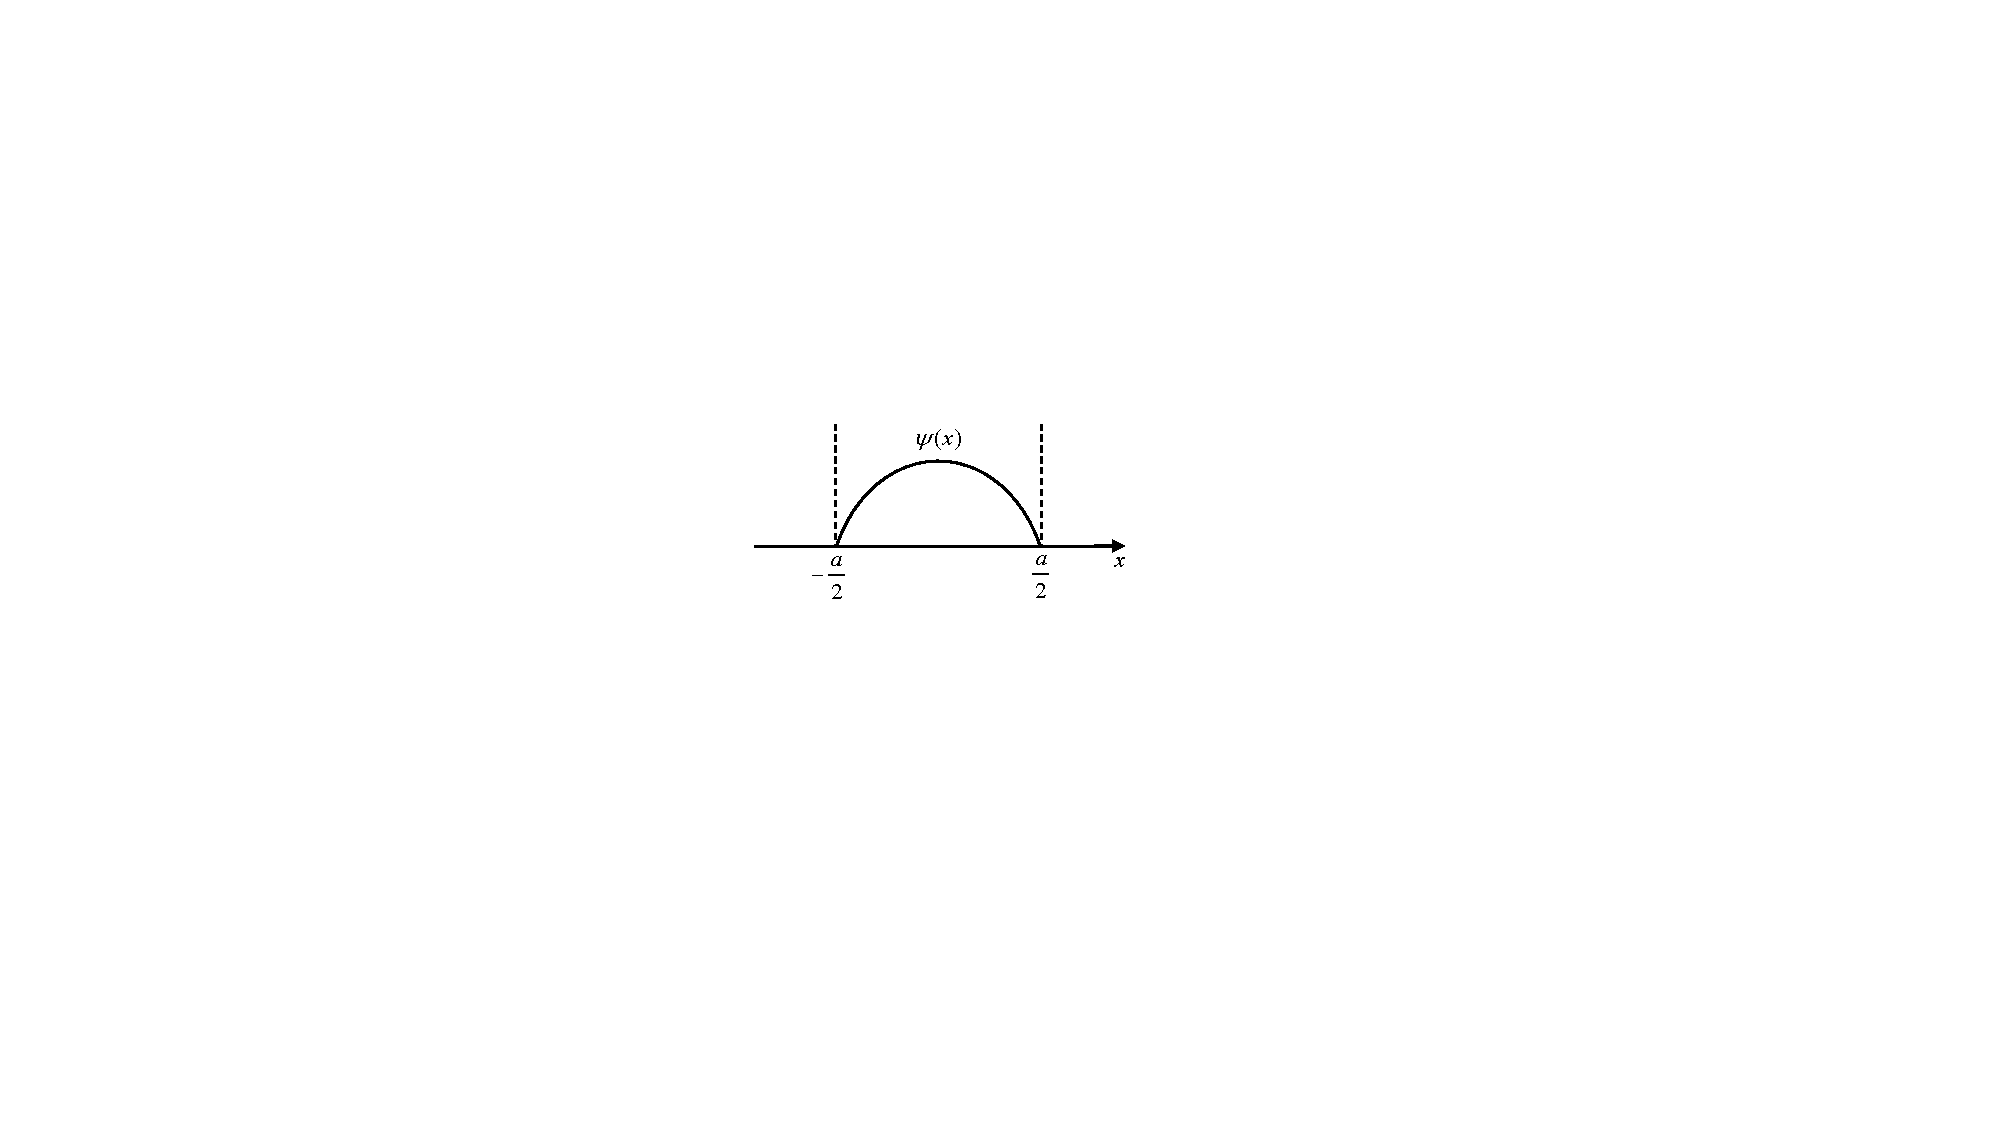
\includegraphics[width=3.5cm]{QM file/figure/3-1}
	\caption{}\label{fig.3-1}
\end{wrapfigure}

\example 如图\ref{fig.3-1},粒子在无限深势阱$\bigg(-\frac{a}{2}<x<\frac{a}{2}\bigg)$中运动,处于基态.如果突然破除势“墙”,而让粒子自由运动,粒子随即在一个方向(例如在$x>\frac{a}{2}$方向)被测量.设测得粒子动能在$(E,E+dE)$范围内的几率为$w(E)dE$,求$w(E)$.

\solution 势“墙”刚破除时,粒子的波函数$\varPsi(x)$就是势阱中的基态波函数,(波函数随时间的变化是连续的,不会突变.)根据\eqref{eq24.10}式,可知
\begin{empheq}{equation}\label{eq35.35}
	\varPsi(x)=
	\begin{dcases}
		\sqrt{\frac{2}{a}}\cos\frac{\pi x}{a},	& |x|<\frac{a}{2}	\\
		0,	& |x|>\frac{a}{2}
	\end{dcases}
\end{empheq}
势“墙”破除后,粒子将在全空间($-\infty<x<\infty$)自由运动.将$\varPsi(x)$展开成动量本征函数的线性叠加:
\begin{empheq}{equation}\label{eq35.36}
	\begin{aligned}
		\varPsi(x)&=\frac{1}{\sqrt{2\pi\hbar}}\int_{-\infty}^{\infty}C(p)e^{ipx/\hbar}dp	\\
		&=\frac{1}{\sqrt{2\pi}}\int_{-\infty}^{\infty}C(k)e^{ikx}dk
	\end{aligned}
\end{empheq}
其中
\begin{empheq}{equation}\label{eq35.37}
	p=\hbar k,\quad dp=\hbar dk,\quad C(k)=\sqrt{\hbar}C(p)
\end{empheq}
按照概率诠释,

$|C(k)|^{2}dk=|C(p)|^{2}dp=$粒子动量在$(p,p+dp)$范围内的概率,粒子自由运动时,能量(动能)和动量的关系是
\begin{empheq}{equation}\label{eq35.38}
	\begin{aligned}
			E	&=\frac{p^{2}}{2m}=\frac{\hbar^{2}k^{2}}{2m}	\\
		dE	&=\frac{\hbar^{2}kdk}{m}
	\end{aligned}
\end{empheq}
因此,
\begin{empheq}{equation*}
	w(E)dE=|C(k)|^{2}dk
\end{empheq}
\begin{empheq}{equation}\label{eq35.39}
	w(E)=|C(k)|^{2}\frac{dk}{dE}=\frac{m|C(k)|^{2}}{\hbar^{2}k}
\end{empheq}
可见关键是求出$C(k)$.按照\eqref{eq35.9}式及\eqref{eq35.37}式、\eqref{eq35.35}式,得
\begin{empheq}{equation}\label{eq35.40}
	\begin{aligned}
		C(k)&=\frac{1}{\sqrt{2\pi}}\int_{-\infty}^{\infty}\varPsi(x)e^{-ikx}dx	\\
		&=\frac{1}{\sqrt{\pi a}}\int_{-\frac{a}{2}}^{\frac{a}{2}}e^{-ikx}\cos\frac{\pi x}{a}dx	\\
		&=\sqrt{\frac{a}{\pi}}\bigg(\frac{1}{\pi-ak}+\frac{1}{\pi+ak}\bigg)\cos\frac{ak}{2}
	\end{aligned}
\end{empheq}
\begin{empheq}{equation}\label{eq35.41}
	|C(k)|^{2}=\frac{4\pi a}{(a^{2}k^{2}-\pi^{2})}\cos^{2}\frac{ak}{2}
\end{empheq}
$\dfrac{|C(k)|^{2}}{\hbar}$就是动量的概率分布函数$|C(p)|^{2}$,$|C(k)|^{2}$随$k$的变化如表\ref{lab.3-1}和图\ref{fig.3-2}所示

\begin{table}[!h]
	\begin{center}
		\caption{}\label{lab.3-1}
		\begin{tabular}{c|c|c|c|c|c|c|c|c}
			\hline 
			\multirow{2}{*}{$\dfrac{ka}{\pi}$} & \multirow{2}{*}{0} & \multirow{2}{*}{0.5} & \multirow{2}{*}{1} & \multirow{2}{*}{1.5} & \multirow{2}{*}{2} & \multirow{2}{*}{3} & \multirow{2}{*}{3.779} & \multirow{2}{*}{5} \\ 
			& & & & & & & & \\ \hline
			\multirow{2}{*}{$|C(k)|^{2}$} & \multirow{2}{*}{$\dfrac{4a}{\pi^{3}}$} & \multirow{2}{*}{$\dfrac{32a}{9\pi^{3}}$} & \multirow{2}{*}{$\dfrac{a}{4\pi}$} & \multirow{2}{*}{$\dfrac{32a}{25\pi^{3}}$} & \multirow{2}{*}{$\dfrac{4}{9\pi^{3}}$} & \multirow{2}{*}{0} & \multirow{2}{*}{\text{(极大)}} & \multirow{2}{*}{0} \\ 
			& & & & & & & & \\ \hline
			\multirow{2}{*}{$|\dfrac{C(k)}{C(0)}|^{2}$} & \multirow{2}{*}{1} & \multirow{2}{*}{$\dfrac{8}{9}$} & \multirow{2}{*}{$\dfrac{\pi^{2}}{16}$} & \multirow{2}{*}{$\dfrac{8}{25}$} & \multirow{2}{*}{$\dfrac{1}{9}$} & \multirow{2}{*}{0} & \multirow{2}{*}{0.005} & \multirow{2}{*}{0} \\ 
			& & & & & & & & \\ \hline
		\end{tabular}
	\end{center}
\end{table}

由图3-2可见,动量分布概率绝大部分集中在$|ka|<2\pi$范围内.如按下式粗略地规定(这样便于计算)分布半宽$\Delta k$,
\begin{empheq}{equation*}
	|C(0)|^{2}2\Delta k=\int_{-\infty}^{\infty}|C(k)|^{2}dk=1
\end{empheq}
则
\begin{empheq}{equation}\label{eq35.42}
	\frac{a}{\hbar}\Delta k=\frac{\pi^{2}}{8}=\num{1.23},\quad\Delta k=\num{1.23}\frac{\pi}{a}
\end{empheq}

\begin{figure}[!h]
	\centering
	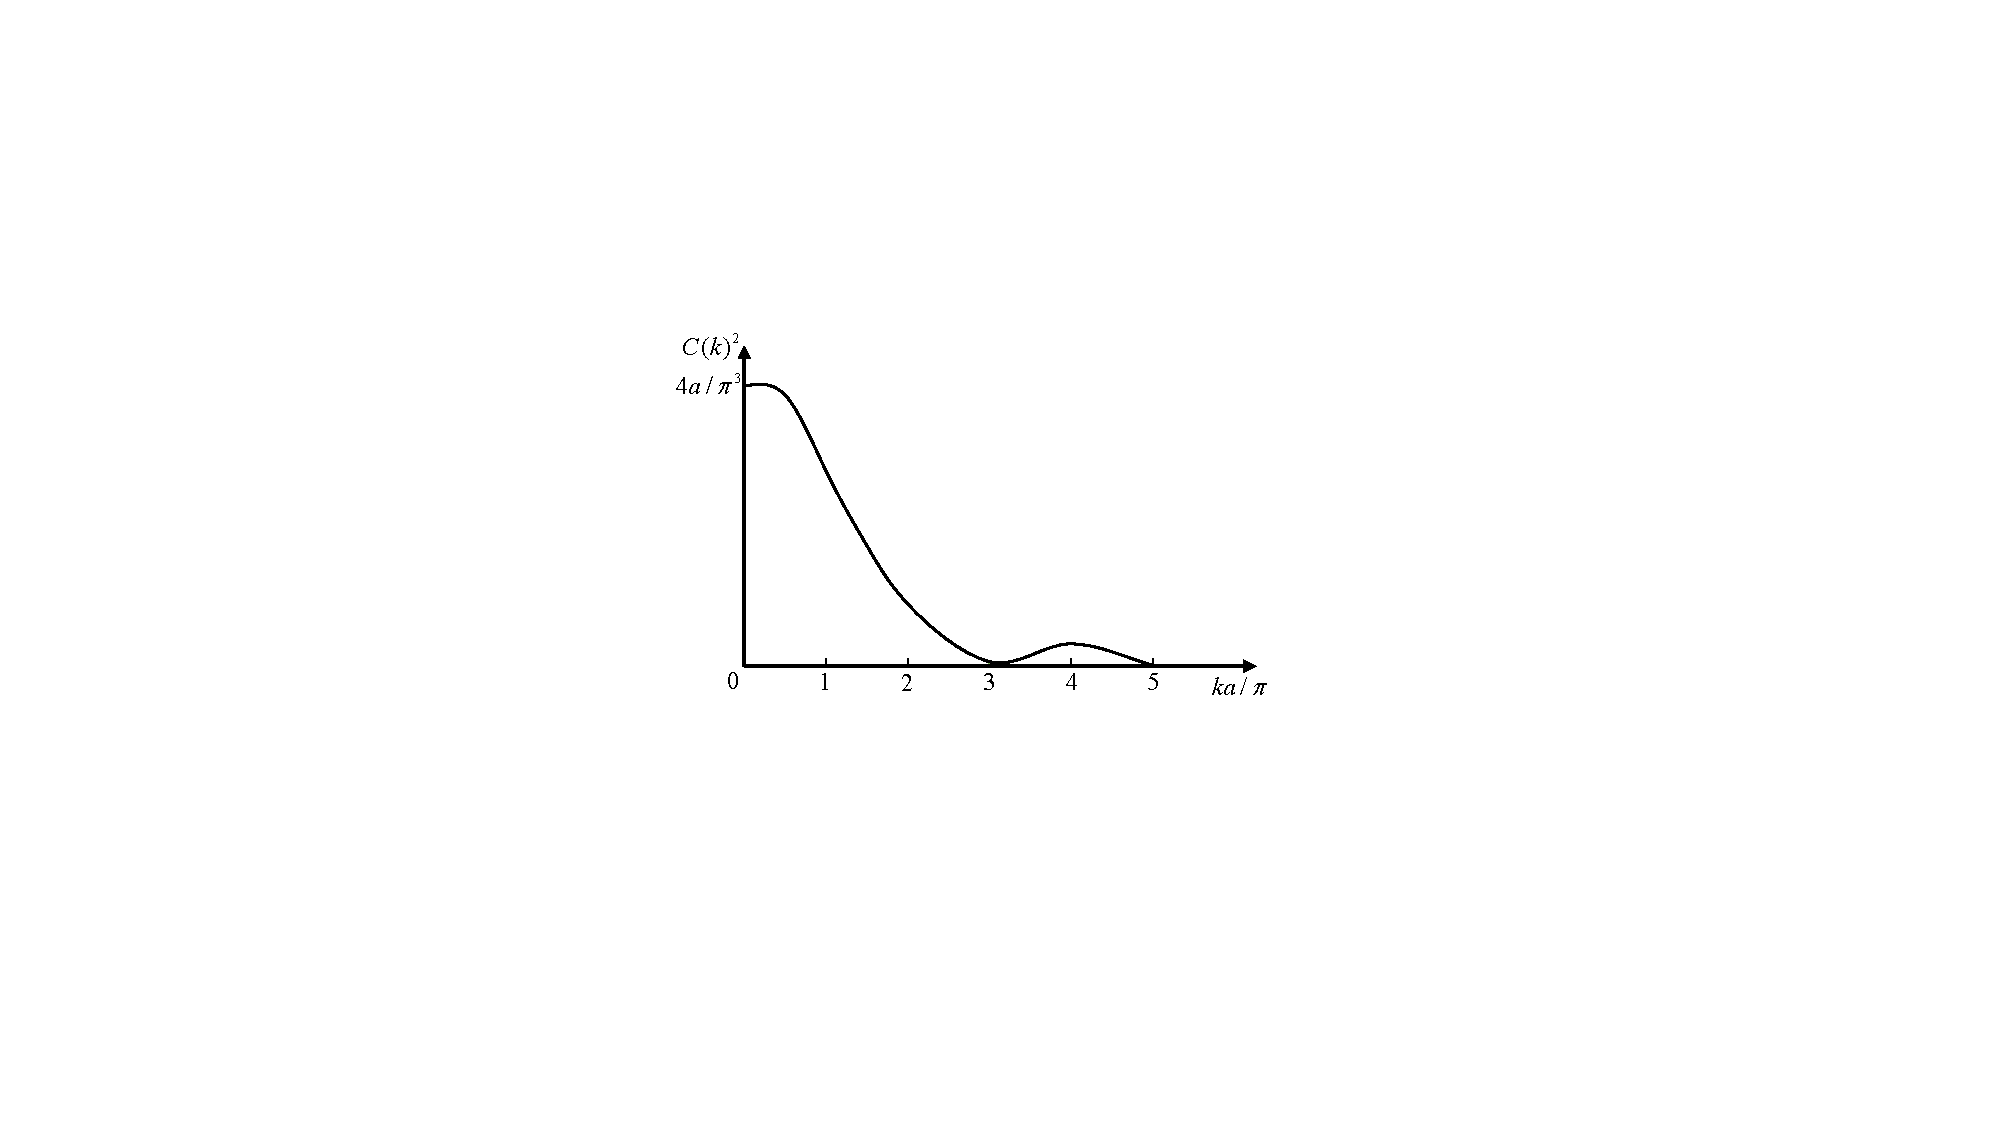
\includegraphics[width=5cm,clip]{QM file/figure/3-2}
	\caption{}\label{fig.3-2}
\end{figure}
$\Delta k$和波函数\eqref{eq35.35}式中的$k=\dfrac{\pi}{a}$很接近.

由\eqref{eq35.39}、\eqref{eq35.41}式求得粒子的动能概率分布函数为
\eqindent{5}
\begin{empheq}{equation}\label{eq35.43}
	\begin{aligned}
		w(E)&=\frac{m}{\hbar^{2}k}\frac{4\pi a}{(a^{2}k^{2}-\pi^{2})}\cos^{2}\frac{ak}{2}	\\
		&=\frac{1}{\hbar}\sqrt{\frac{m}{2E}}\frac{4\pi a}{\bigg(\frac{a^{2}}{\hbar^{2}}2mE-\pi^{2}\bigg)^{2}}\cos^{2}\frac{a}{\hbar}\sqrt{\frac{mE}{2}}
	\end{aligned}
\end{empheq}\eqnormal
用围道积分法不难验证:
\begin{empheq}{equation}\label{eq35.44}
	2\int_{0}^{\infty}w(E)dE=\int_{-\infty}^{\infty}|C(k)|^{2}dk=1
\end{empheq}



% 力学量算符的对易关系式
\section[力学量算符的对易关系式]{力学量算符的对易关系式} \label{sec:03.06} % 
% \makebox[5em][s]{} % 短题目拉间距

许多量子力学问题都涉及到力学蜇算符之间的对易关系式.最基本的就是位置算符和动量算符之间的对易关系式(见$\S$\ref{sec:03.02}):
\eqindent{10}
\begin{empheq}{align}	%1,2,3
	\hat{p_{x}}\hat{p_{y}}-\hat{p_{y}}\hat{p_{x}}=0	\label{eq36.1} \\%1
	\hat{x}\hat{p_{x}}-\hat{p_{x}}\hat{x}=i\hbar	\label{eq36.2} \\%2
	\hat{x}\hat{p_{y}}-\hat{p_{y}}\hat{x}=0			\label{eq36.3}	 %3
\end{empheq}
等等.为了便于运算,定义算符$\hat{A},\hat{B}$之间的对易式(又称量子括号):
\begin{empheq}{equation}\label{eq36.4}
	[\hat{A},\hat{B}]\equiv\hat{A}\hat{B}-\hat{B}\hat{A}
\end{empheq}\eqnormal
\eqindent{12}
则\eqref{eq36.1}、\eqref{eq36.2}、\eqref{eq36.3}式可以写成
\begin{empheq}{align*}	%1',2',3'
	[\hat{p_{x}},\hat{p_{y}}]&=0		\tag{$3.6.1^{\prime}$} \label{eq36.1'} \\
	[\hat{x}\hat{p_{x}}]&=i\hbar		\tag{$3.6.2^{\prime}$} \label{eq36.2'} \\
	[\hat{x}\hat{p_{y}}]&=0			\tag{$3.6.3^{\prime}$} \label{eq36.3'}
\end{empheq}\eqnormal
根据定义\eqref{eq36.4}式,容易证明以下运算规则:
\eqindent{6}
\begin{gather}
	[\hat{A},\hat{B}]=-[\hat{B},\hat{A}]	\label{eq36.5}\\ %5
	[\hat{A},\hat{B}+\hat{C}]=[\hat{A},\hat{B}]+[\hat{A},\hat{C}]	\label{eq36.6}\\ %6
	[\hat{A}+\hat{B},\hat{C}]=[\hat{A},\hat{C}]+[\hat{B},\hat{C}]	\label{eq36.7}\\ %7
	[\hat{A},\hat{B}\hat{C}]=[\hat{A},\hat{B}]\hat{C}+\hat{B}[\hat{A},\hat{C}]	\label{eq36.8}\\ %8
	[\hat{A}\hat{B},\hat{C}]=[\hat{A},\hat{C}]\hat{B}+\hat{A}[\hat{B},\hat{C}]	\label{eq36.9}\\ %9
	[\hat{A},[\hat{B},\hat{C}]]+[\hat{B}[\hat{C},\hat{A}]]+[\hat{C}[\hat{A},\hat{B}]]=0	\label{eq36.10} %10		
\end{gather}
熟练地掌握这些公式,计算就能进行得正确而迅速.例如利用\eqref{eq36.8}式及\eqref{eq36.2'}式,
可得
\begin{align}%11,12
	[\hat{x},\hat{p_{x}}^{2}] &=[\hat{x},\hat{p_{x}}]\hat{p_{x}}+\hat{p_{x}}[\hat{x},\hat{p_{x}}]=2i\hbar\hat{p_{x}}	\label{eq36.11}\\ %11
	[\hat{x},\hat{p_{x}}^{3}] &=[\hat{x},\hat{p_{x}}]\hat{p_{x}}^{2}+\hat{p_{x}}[\hat{x},\hat{p_{x}}^{2}]=3i\hbar\hat{p_{x}}^{2}	\label{eq36.12} %12
\end{align}\eqnormal
依此类推,对于任何正整数$n$,可证
\begin{empheq}{equation}\label{eq36.13}
	[\hat{x},\hat{p_{x}}^{n}]=i\hbar n\hat{p_{x}}^{n-1}=i\hbar\frac{\partial\hat{p_{x}}^{n}}{\partial\hat{p_{x}}}
\end{empheq}
再考虑到\eqref{eq36.3'}式,可知对于任何可以展开成$\hat{p_{x}},\hat{p_{y}},\hat{p_{z}}$正幕级数的算符$\hat{F(\boldsymbol{p})}$,有
下列对易关系式:
\begin{empheq}{equation}\label{eq36.14}
	[\hat{x},\hat{F(\boldsymbol{p})}]=i\hbar\frac{\partial\hat{F}}{\partial\hat{p_{x}}}
\end{empheq}
类似地,对于任意函数(作为算符)$f(\boldsymbol{r})$,有对易式
\begin{empheq}{equation}\label{eq36.15}
	[\hat{p_{x}},f(\boldsymbol{r})]=-i\hbar\frac{\partial f}{\partial x}
\end{empheq}

与轨道角动量算符$\hat{\boldsymbol{L}}=\boldsymbol{r}\times\boldsymbol{p}$有关的对易式应用极广,例如:
\eqindent{6}
\begin{empheq}{align}%16,17,18
	&[\hat{x},\hat{L_{x}}]=[\hat{x},\hat{y}\hat{p_{z}}]-[\hat{x},\hat{z}\hat{p_{y}}]=0	\label{eq36.16}\\
	&[\hat{x},\hat{L_{y}}]=[\hat{x},\hat{z}\hat{p_{x}}]-[\hat{x},\hat{x}\hat{p_{z}}]=\hat{z}[\hat{x},\hat{p_{x}}]=i\hbar\hat{z}	\label{eq36.17}\\
	&[\hat{L_{x}},\hat{y}]=[\hat{y}\hat{p_{z}},\hat{y}]-[\hat{z}\hat{p_{y}},\hat{y}]=-\hat{z}[\hat{p_{y}},\hat{y}]=i\hbar\hat{z}	\label{eq36.18}
\end{empheq}
类似地,可以证明
\begin{empheq}{equation}\label{eq36.19}
	[\hat{p_{x}},\hat{L_{x}}]=0,\quad[\hat{p_{x}},\hat{L_{y}}]=[\hat{L_{x}},\hat{p_{y}}]=i\hbar\hat{p_{z}}
\end{empheq}\eqnormal
等等.以上各式经过$(x\rightarrow y,y\rightarrow z,z\rightarrow x)$轮换后,仍旧成立.例如,\eqref{eq36.17}式和\eqref{eq36.18}式的轮换式是
\begin{empheq}{align*}
	[\hat{y},\hat{L_{z}}]=[\hat{L_{y}},\hat{z}]=i\hbar\hat{x}	\tag{$3.6.17^{\prime}$} \label{eq36.17'} \\
	[\hat{z},\hat{L_{x}}]=[\hat{L_{z}},\hat{x}]=i\hbar\hat{y}	\tag{$3.6.18^{\prime}$} \label{eq36.18'} 
\end{empheq}
\eqref{eq36.16}式的轮换式是
\begin{empheq}{equation*}\label{eq36.16'}
	[\hat{y},\hat{L_{y}}]=0,\quad [\hat{z},\hat{L_{z}}]=0	\tag{$3.6.16^{\prime}$} 
\end{empheq}

利用以上各式,就可以计算角动量算符$\hat{\boldsymbol{L}}$的各个分量之间的对易式,例如:
\eqindent{6}
\begin{empheq}{equation}\label{eq36.20}
	\begin{aligned}
		[\hat{L_{x}},\hat{L_{y}}]&=[\hat{y}\hat{p_{z}},\hat{L_{y}}]-[\hat{z}\hat{p_{y}},\hat{L_{y}}]	\\
		&=\hat{y}[\hat{p_{z}},\hat{L_{y}}]-[\hat{z},\hat{L_{y}}]\hat{p_{y}}	\\
		&=i\hbar(-\hat{y}\hat{p_{x}}+\hat{x}\hat{p_{y}})=i\hbar\hat{L_{z}}
	\end{aligned}
\end{empheq}\eqnormal
\eqref{eq36.20}式及其轮换式常被写成矢量形式:
\eqindent{12}
\begin{empheq}{equation}\label{eq36.21}
	\boxed{\hat{\boldsymbol{L}}\times\hat{\boldsymbol{L}}=i\hbar\hat{\boldsymbol{L}}}
\end{empheq}\eqnormal
利用\eqref{eq36.20}式或\eqref{eq36.21}式,可以进一步证明:
\begin{empheq}{equation}\label{eq36.22}
	[\hat{L_{\alpha}},\hat{\boldsymbol{L}}^{2}]=0,\quad \alpha=x,y,z
\end{empheq}
写成矢量形式,就是\eqindent{12}
\begin{empheq}{equation*}\label{eq36.22'}
	[\hat{\boldsymbol{L}},\hat{\boldsymbol{L}}^{2}]=0	\tag{$3.6.22^{\prime}$}
\end{empheq}\eqnormal
\eqref{eq36.21}、\eqref{eq36.22}式是角动蜇算符最本质的关系式.尤其是\eqref{eq36.21}式,是经典物理中根本不可能有的关系.在经典物理中,所有物理量都是普通数量,当然都是互相对易的,因此对于任何向量$\boldsymbol{A}$,总有$\boldsymbol{A}\times\boldsymbol{A}=0$.而作为量子力学算符的角动量$\hat{\boldsymbol{L}}$,各分量不对易,满足\eqref{eq36.21}式,由此决定了角动量的一系列异乎寻常的性质.$\S$\ref{sec:04.07}将详细讨论这个问题.

利用\eqref{eq36.16}至\eqref{eq36.19}式容易证明:
\begin{empheq}{equation}\label{eq36.23}
	[\hat{L_{\alpha}},\boldsymbol{r}^{2}]=0,\quad[\hat{L_{\alpha}},\hat{\boldsymbol{p}}^{2}]=0,\quad \alpha=x,y,z
\end{empheq}
亦即
\begin{empheq}{equation*}\label{eq36.23'}
	[\hat{\boldsymbol{L}},\boldsymbol{r}^{2}]=0,\quad [\hat{\boldsymbol{L}},\hat{\boldsymbol{p}}^{2}]=0	\tag{$3.6.23^{\prime}$}
\end{empheq}
利用$\hat{\boldsymbol{L}}$的球坐标表示式[\eqref{eq31.15}式],容易看出
\begin{empheq}{equation}\label{eq36.24}
	[\hat{\boldsymbol{L}},\hat{f(r)}]=0
\end{empheq}
$\hat{f(r)}$是任何径向函数(作为算符).总之,角动量算符$\hat{\boldsymbol{L}}$和任何标量(转动不变量)算符对易.

\example 选定任意两个空间方向,以$n,m$表示这两个方向的单位矢量:
\begin{empheq}{equation*}
	\boldsymbol{n}=(n_{x},n_{y},n_{z}),\quad\boldsymbol{m}=(m_{x},m_{y},m_{z})
\end{empheq}
定义角动量算符在$\boldsymbol{n},\boldsymbol{m}$方向的投影
\begin{empheq}{align*}
	\hat{L_{n}}&=\boldsymbol{n}\cdot\hat{\boldsymbol{L}}=n_{x}\hat{L_{x}}+n_{y}\hat{L_{y}}+n_{z}\hat{L_{z}}	\\
	\hat{L_{m}}&=\boldsymbol{m}\cdot\hat{\boldsymbol{L}}=m_{x}\hat{L_{x}}+m_{y}\hat{L_{y}}+m_{z}\hat{L_{z}}
\end{empheq}
试计算对易式$[\hat{L_{n}},\hat{L_{m}}]$.

\begin{wrapfigure}[6]{r}{7em}
	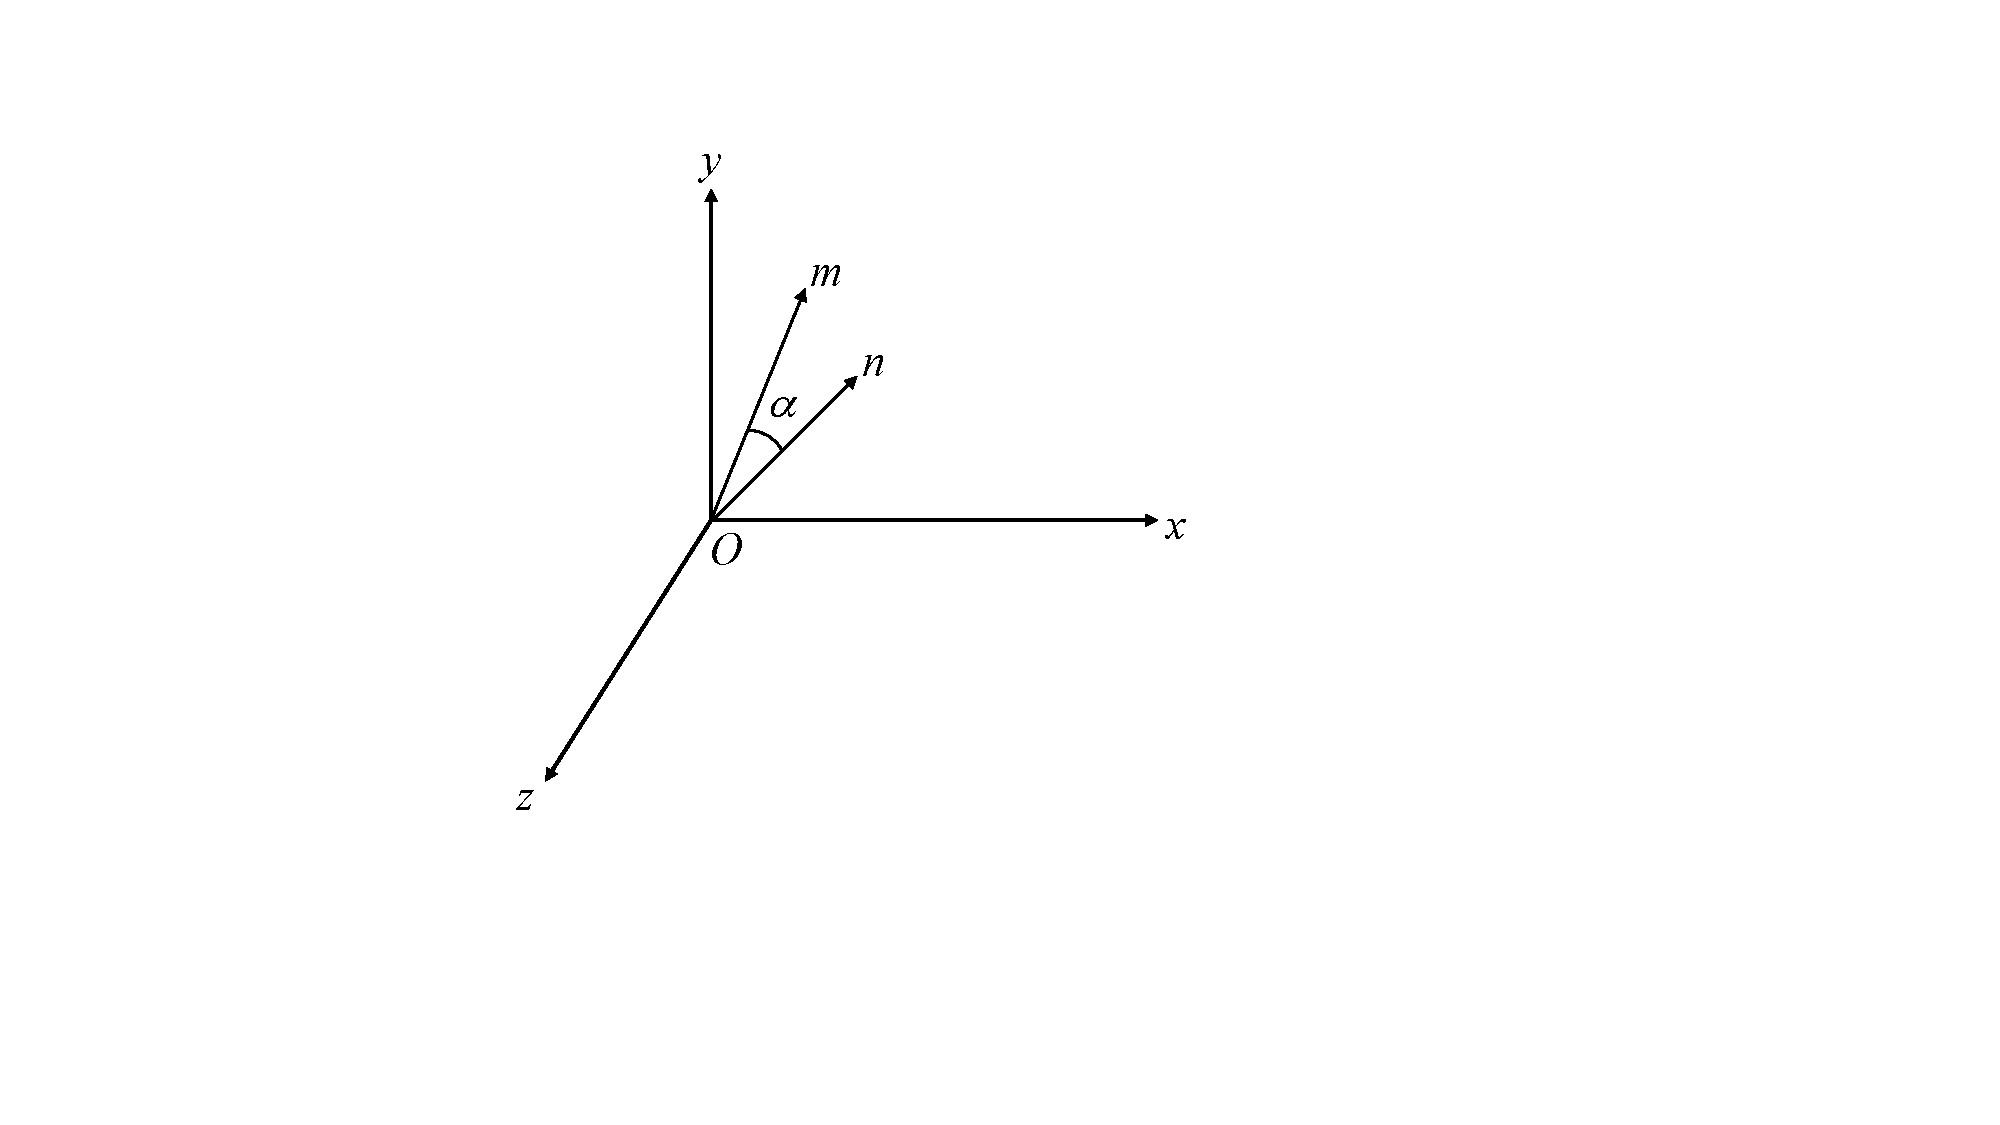
\includegraphics[width=3cm]{QM file/figure/3-3}
	\caption{}\label{fig.3-3}
\end{wrapfigure}

\solution 利用基本对易式\eqref{eq36.21},可得
\eqindent{2}
\begin{align}\label{eq36.25}
	[\hat{L_{n}},\hat{L_{m}}]& = n_{x}m_{y}[\hat{L_{x}},\hat{L_{y}}]+n_{y}m_{x}[\hat{L_{y}},\hat{L_{x}}]+\cdots	\nonumber\\
	&= (n_{x}m_{y}-n_{y}m_{x})i\hbar\hat{L_{z}}+\cdots	\nonumber\\
	&= i\hbar(\boldsymbol{n}\times\boldsymbol{m})_{z}\hat{L_{z}}+\cdots	\nonumber\\
	&= i\hbar(\boldsymbol{n}\times\boldsymbol{m})\cdot\hat{\boldsymbol{L}}
\end{align}\eqnormal
如以$\alpha$表示$(\boldsymbol{n},\boldsymbol{m})$夹角,$\boldsymbol{l}$表示$(\boldsymbol{n}\times\boldsymbol{m})$方向单位矢量,上式可以写成
\begin{empheq}{equation*}\label{eq36.25'}
	[\hat{L_{n}},\hat{L_{m}}]=i\hbar\hat{L_{l}}\sin\alpha
\end{empheq}
如果$\boldsymbol{n},\boldsymbol{m}$在$x-y$平面上,则$\boldsymbol{n}\times\boldsymbol{m}$指向$z$轴,如图\ref{fig.3-3}所示,上式成为
\begin{empheq}{equation}\label{eq36.26}
	[\hat{L_{n}},\hat{L_{m}}]=i\hbar\hat{L_{z}}\sin\alpha
\end{empheq}
其中角$\alpha$定义为由$\boldsymbol{n}$方向开始,沿逆时针方向转到$\boldsymbol{m}$方向所经历的角度($\alpha$可以大于$\pi$).





% 两个力学量算符的共同本征态
\section[两个力学量算符的共同本征态]{两个力学量算符的共同本征态} \label{sec:03.07} % 
% \makebox[5em][s]{} % 短题目拉间距

考虑物理体系(最简单的情况就是一个粒子)的两种力学量(可观测量)$A$,$B$.设在某种状态下,$A$和$B$都有确定的取值,$A=a_{n},B=b_{k}$.(为了叙述方便,设本征值谱是分立的)根据本征态和本征值的物理解释,可知这个状态既是算符$\hat{A}$的本征态,又是$\hat{B}$的本征态,亦即是$\hat{A}$和$\hat{B}$的共同本征态.相应的波函数记为$\varPsi_{nk}$,满足本征方程
\begin{empheq}{equation}\label{eq37.1}
	\hat{A}\varPsi_{nk}=a_{n}\varPsi_{nk},\quad \hat{B}\varPsi_{nk}=b_{k}\varPsi_{nk}
\end{empheq}
因此
\begin{empheq}{equation}\label{eq37.2}
	(\hat{A}\hat{B}-\hat{B}\hat{A})\varPsi_{nk}=(a_{n}b_{k}-b_{k}a_{n})\varPsi_{nk}=0
\end{empheq}
这结果提示我们,$\hat{A}$和$\hat{B}$可能是对易算符.但是,如$\hat{A},\hat{B}$仅存在个别的共同本征态,并不能由此得出$\hat{A},\hat{B}$是对易算符的结论.

如果$\hat{A},\hat{B}$存在一系列共同本征函数,构成完备函数系,情况就不同了.这时任何波函数$\varPsi$都可以表示成这些共同本征函数的线性叠加:
\begin{empheq}{equation}\label{eq37.3}
	\varPsi=\sum_{n,k}C_{nk}\varPsi_{nk}
\end{empheq}
从而
\begin{empheq}{equation*}
	(\hat{A}\hat{B}-\hat{B}\hat{A})\varPsi=\sum_{n,k}C_{nk}(\hat{A}\hat{B}-\hat{B}\hat{A})\varPsi_{nk}=0
\end{empheq}
由此可得
\begin{empheq}{equation}\label{eq37.4}
	\hat{A}\hat{B}-\hat{B}\hat{A}=[\hat{A},\hat{B}]=0
\end{empheq}
即$\hat{A},\hat{B}$为对易算符.

反过来,如果力学量算符$\hat{A},\hat{B}$对易,即$\hat{A}\hat{B}=\hat{B}\hat{A}$,则$\hat{A}$和$\hat{B}$必定存在一系列共同本征函数,并构成完全函数系证明如下.

由于$\hat{A}$和$\hat{B}$都是力学量算符,它们各自存在一组完备的本征函数系,记为$|\varPsi_{n}|$和$|\Phi_{k}|$,满足本征方程:
\begin{empheq}{align}%5,6
	\hat{A}\varPsi_{n}&=a_{n}\varPsi_{n},\quad n=1,2,3,\cdots	\label{eq37.5}\\
	\hat{B}\Phi_{k}&=b_{k}\Phi_{k},\quad k=1,2,3,\cdots	\label{eq37.5}
\end{empheq}
$n$和$k$为本征函数的编号数,对于简并态,本征值重复出现.任取一个$\hat{A}$的本征函数$\varPsi_{n}$,将它表示成$\hat{B}$的本征函数的线性叠加:
\begin{empheq}{equation}\label{eq37.7}
	\varPsi_{n}=\sum_{k}C_{nk}\Phi_{k}=\sum_{i}\tilde{\Phi_{i}}
\end{empheq}
考虑到可能存在的简并化,上式中$\tilde{\Phi_{i}}$表示$\sum_{k}$中相应于$\hat{B}$的同一个本征值$b_{i}$的各项之和(对于$\sum_{k}$中的非简并项,$\tilde{\Phi_{i}}$就是$C_{ni}\Phi_{i}$),因此
\begin{empheq}{equation}\label{eq37.8}
	\hat{B}\tilde{\Phi_{i}}=b_{i}\tilde{\Phi_{i}}
\end{empheq}
\eqref{eq37.7}式中各$\tilde{\Phi_{i}}$,相应于$\hat{B}$的不同本征值,因而是互相线性独立的.下面证明每个$\tilde{\Phi_{i}}$都是$\hat{A}$的本征函数.将\eqref{eq37.7}式代入\eqref{eq37.5}式,得到
\begin{empheq}{equation}\label{eq37.9}
	(\hat{A}-a_{n})\varPsi_{n}=\sum_{i}(\hat{A}-a_{n})\tilde{\Phi_{i}}=0
\end{empheq}
以算符$\hat{B}$作用于上式中每一项,由于$\hat{A},\hat{B}$对易,得到
\begin{empheq}{equation*}
	\hat{B}(\hat{A}-a_{n})\tilde{\Phi_{i}}=(\hat{A}-a_{n})\hat{B}\tilde{\Phi_{i}}=b_{i}(\hat{A}-a_{n})\tilde{\Phi_{i}}
\end{empheq}
上式表明,$(\hat{A}-a_{n})\tilde{\Phi_{i}}$如果不等于0,它就是$\hat{B}$的本征函数,相应于本征值$b_{i}$;而\eqref{eq37.9}式意味着相应于$\hat{B}$的不同本征值的本征函数是线性相关的!这当然是不可能的.为了避免这个矛盾,必须
\begin{empheq}{equation}\label{eq37.10}
	(\hat{A}-a_{n})\tilde{\Phi_{i}}=0
\end{empheq}
因此$\tilde{\Phi_{i}}$是$\hat{A}$的本征函数,相应于本征值$a_{n}$.至此已经证明了$\tilde{\Phi_{i}}$是$\hat{A},\hat{B}$的共同本征函数.这就是说,$\hat{A}$的每一个本征函数$\varPsi_{n}$都可以分解成若干个$\hat{A},\hat{B}$的共同本征函数$\tilde{\Phi_{i}}$.由于全体$|\varPsi_{n}|$是完备函数系,显然全体$\tilde{\Phi_{i}}$也是完备函数系.证明完毕.

从上面的论证可以得出一个直接的推论,即, 如$\hat{A},\hat{B}$对易, 而$\hat{A}$或$\hat{B}$具有某些非简并本征函数,则它们必然是$\hat{A},\hat{B}$的共同本征函数.

如果算符$\hat{A}$的全部本征函数都是非简并的,而算符$\hat{B}$和$\hat{A}$对易,则$\hat{A}$的每一个本征函数同时也是$\hat{B}$的本征函数,因此$\hat{B}$的本征值逐个取决于$\hat{A}$的本征值,从而可以认为力学量$B$是力学量$A$的函数.这样,凡是与$\hat{A}$对易的厄密算符,必定是$\hat{A}$的函数.如力学量$B$不是$A$的函数,则称$\hat{B}$独立于$\hat{A}$,显然$\hat{B}$和$\hat{A}$必定是不可对易的.

如果$\hat{A}$的一部分或全部本征函数是简并的,则给定$\hat{A}$的本征值并不足以完全确定波函数.这种情况下必然存在独立于$\hat{A}$而又与$\hat{A}$对易的其他力学量算符$\hat{B}$,它们存在共同本征函数,并构成完备函数系.如果$\hat{A},\hat{B}$的共同本征函数仍有简并,则给定$\hat{A},\hat{B}$的本征值仍不足以完全确定波函数,这时必定还存在独立于$\hat{A},\hat{B}$而又与$\hat{A},\hat{B}$对易的其他力学量算符.依此类推.

一组互相对易而又互相独立的力学量算符,如它们的共同本征函数是非简并的,并且构成完备函数系,则这组力学量称为力学量完全集,它们的一组本征值唯一地确定出一个共同本征态.构成完全集的独立力学量数目,称为物理体系的自由度.例如,一维谐振子,总能量算符$\hat{H}$的本征函数全部是非简并的,因此$H$本身就是力学量完全集,自由度为1.又如三维自由粒子,力学量完全集可以取为$(p_{x},p_{y},p_{z})$,总能量算符$\hat{H}=\hat{\boldsymbol{p}}^{2}/2m$是它们的函数,它们的共同本征函数$\varPsi_{\boldsymbol{p}}$[\eqref{eq35.10}式]就是通常说的平面波波函数;也可以选取别的力学量完全集,如$(\boldsymbol{p}^{2},\boldsymbol{L}^{2},L_{z})$,它们的共同本征态俗称自由粒子球面波,将在$\S$\ref{sec:05.02}讨论.

必须指出,两个或多个互不对易的力学量算符,也可能存在个别的共同本征函数,但是不足以构成完备函数系.设$\hat{A},\hat{B}$为力学量算符(厄密算符),不对易,设
\begin{empheq}{equation}\label{eq37.11}
	[\hat{A},\hat{B}]=\hat{A}\hat{B}-\hat{B}\hat{A}=i\hat{C}
\end{empheq}
容易证明$\hat{C}$是厄密算符.设$\varPsi_{ab}$是$\hat{A},\hat{B}$的共同本征函数,相应于本征值$A=a$,$B=b$.将\eqref{eq37.11}式作用于$\varPsi_{ab}$,易得
\begin{empheq}{equation}\label{eq37.12}
	\hat{C}\varPsi_{ab}=0
\end{empheq}
即$\varPsi_{ab}$也是算符$\hat{C}$的本征函数,本征值为0.所以,如果算符$\hat{C}$的本征值谱中不包含0,$\hat{A},\hat{B}$就没有共同本征函数.例如$\hat{A}=\hat{x},\hat{B}=\hat{p_{x}}$,$[\hat{x},\hat{p_{x}}]=i\hbar$,即$\hat{C}=\hbar$,$\hat{C}$的唯一本征值就是$\hbar$,所以$\hat{x}$和$\hat{p_{x}}$没有共同本征函数.注意,\eqref{eq37.12}式仅是$\hat{A},\hat{B}$的共同本征函数所必须满足的必要条件,并非充分条件.

\example 讨论轨道角动量$\boldsymbol{L}=\boldsymbol{r}\times\boldsymbol{p}$的任何两个分量存在共同本征函数的可能性,并求出这种共同本征函数.

\solution 算符$\hat{\boldsymbol{L}}$的三个分量互不对易,满足对易式:
\eqindent{4}
\begin{empheq}{equation}\label{eq37.13}
	[\hat{L_{x}},\hat{L_{y}}]=i\hbar\hat{L_{z}},\quad[\hat{L_{y}},\hat{L_{x}}]=i\hbar\hat{L_{x}},\quad[\hat{L_{z}},\hat{L_{x}}]=i\hbar\hat{L_{y}}
\end{empheq}\eqnormal
设$\varPsi$为$\hat{L_{x}}$,$\hat{L_{y}}$的共同本征征函数,以\eqref{eq37.13}第一式作用于$\varPsi$,得到
\begin{empheq}{equation}\label{eq37.14}
	\hat{L_{z}}\varPsi=0
\end{empheq}
再以\eqref{eq37.13}第二式和第三式作用于$\varPsi$,得到
\begin{empheq}{equation*}\label{eq37.14'}
	\hat{L_{x}}\varPsi=0,\quad\hat{L_{y}}\varPsi=0
\end{empheq}
所以,$\hat{\boldsymbol{L}}$的任何两个分量的共同本征函数,必为三个分量的共同本征函数,本征值全部等于0,亦即$\varPsi$满足
\begin{empheq}{equation}\label{eq37.15}
	\hat{\boldsymbol{L}}\varPsi=-i\hbar\boldsymbol{r}\times\nabla\varPsi=0
\end{empheq}
因此$\nabla\varPsi$的方向和$\boldsymbol{r}$平行.满足这条件的$\varPsi$必须是径向函数,即
\begin{empheq}{equation}\label{eq37.16}
	\varPsi=\varPsi(r)\quad\text{(与$\theta,\varphi$无关)}
\end{empheq}
这就是$\hat{\boldsymbol{L}}$的三个分量的共同本征函数.显然,\eqref{eq37.16}式并不构成完全函数系,它不
能表示与方向$(\theta,\varphi)$有关的波函数.














% 不确定度关系
\section[不确定度关系]{不确定度关系} \label{sec:03.08} % 
% \makebox[5em][s]{} % 短题目拉间距

考虑两个力学量$A,B$及其算符$\hat{A},\hat{B}$,任意给定一个归一化的波函数$\varPsi$.如$\varPsi$是$\hat{A}$或$\hat{B}$的本征函数,则力学量$A$或$B$将取单一的本征值,这种情况不予讨论.如$\varPsi$不是$\hat{A}$或$\hat{B}$的本征函数,则$A$和$B$的取值均将具有某种分布,定义分布宽度(涨落)$\Delta A$,$\Delta B$,
\begin{empheq}{equation}\label{eq38.1}
	\begin{aligned}
		(\Delta A)^{2}&=\overline{(\hat{A}-\bar{A})^{2}}=\overline{A^{2}}-\bar{A}^{2}	\\
		(\Delta B)^{2}&=\overline{(\hat{B}-\bar{B})^{2}}=\overline{B^{2}}-\bar{B}^{2}
	\end{aligned}
\end{empheq}
试问,对于各种不同的波函数$\varPsi$,$\Delta A\cdot\Delta B$的下限是什么?如果$\hat{A},\hat{B}$对易,可取$\varPsi$尽量接近$\hat{A},\hat{B}$的共同本征函数,使$\Delta A,\Delta B$都很小,所以$\Delta A\cdot\Delta B$的下限为0.如$\hat{A},\hat{B}$不对易,令
\begin{empheq}{equation}\label{eq38.2}
	[\hat{A},\hat{B}]\equiv\hat{A}\hat{B}-\hat{B}\hat{A}=i\hat{C}
\end{empheq}
$\hat{C}$必为厄密算符,它在$\varPsi$态下的平均值
\begin{empheq}{equation}\label{eq38.3}
	\bar{C}=-i\int\varPsi^{*}(\hat{A}\hat{B}-\hat{B}\hat{A})\varPsi d\tau
\end{empheq}
必为实数,可以证明
\begin{empheq}{equation}\label{eq38.4}
	\boxed{\Delta A\cdot\Delta B\geqslant\frac{1}{2}|\bar{C}|}
\end{empheq}
称为不确定度关系(曾称为测不准关系).\eqref{eq38.4}式的证明如下.

对于任意线性算符$\hat{F}$及其共轭$\hat{F}^{*}$,$\hat{F}^{*}\hat{F}$的平均值为
\eqindent{6}
\begin{empheq}{align}\label{eq38.5}
	\overline{\hat{F}^{*}\hat{F}}&=\int\varPsi^{*}\hat{F}^{*}\hat{F}\varPsi d\tau	\nonumber\\
	&=\int(\hat{F}\varPsi)(\hat{F}\varPsi)^{*}d\tau=\int|\hat{F}\varPsi|^{2}d\tau\geqslant 0
\end{empheq}\eqnormal
令
\begin{empheq}{equation}\label{eq38.6}
	\hat{F}=\hat{A}+i\xi\hat{B}
\end{empheq}
$\xi$为实参数(注意,如$A,B$量纲相同,$\xi$是无量纲参数;如$A,B$量纲不同,则$\xi$有量纲.)
\eqindent{6}
\begin{empheq}{align}\label{eq38.7}
	\hat{F}^{*}\hat{F}&=(\hat{A}-i\xi\hat{B})(\hat{A}+i\xi\hat{B})	\nonumber\\
		&=\hat{A}^{2}+\xi^{2}\hat{B}^{2}+i\xi[\hat{A},\hat{B}]=\hat{A}^{2}+\xi^{2}\hat{B}^{2}-\xi\hat{C}
\end{empheq}\eqnormal
代入\eqref{eq38.5}式, 即得
\begin{empheq}{equation}\label{eq38.8}
	\overline{A^{2}}+\xi^{2}\overline{B^{2}}-\xi\overline{C}\geqslant 0
\end{empheq}
等号成立的条件为
\begin{empheq}{equation}\label{eq38.9}
	\hat{F}\varPsi=(\hat{A}+i\xi\hat{B})\varPsi=0
\end{empheq}
\eqref{eq38.8}式对任何$\xi$值(实数),任何归一化波函数$\varPsi$,均可成立.但如$\varPsi$是$\hat{A}$或$\hat{B}$的本征函数,这时$\bar{C}=0$,\eqref{eq38.8}式没有实际价值.

\eqref{eq38.8}式中取$\xi=\pm 1$(如$\bar{C}>0$,取$\xi=1$;如$\bar{C}<0$,取$\xi=-1$)得到
\begin{empheq}{equation}\label{eq38.10}
	\overline{A^{2}}+\overline{B^{2}}\geqslant|\bar{C}|
\end{empheq}
\eqref{eq38.8}式中取$\xi=\bar{C}/(2\overline{B^{2}})$或$\xi=\pm\sqrt{\overline{A^{2}}/\overline{B^{2}}}$($\bar{C}>0$,取正号;$\bar{C}<0$,取负号),得到
\begin{empheq}{equation}\label{eq38.11}
	\overline{A^{2}}\overline{B^{2}}\geqslant\frac{1}{4}\bar{C}^{2}
\end{empheq}
这实际上是\eqref{eq38.8}式成立的充要条件.\eqref{eq38.11}式其实已经包含了\eqref{eq38.10}式.

\eqref{eq38.8}至\eqref{eq38.11}式适用于任何厄密算符$\hat{A},\hat{B}$.如将$\hat{A}$换成$(\hat{A}-\bar{A})$,$\hat{B}$换成$(\hat{B}-\bar{B})$,则
\begin{empheq}{align*}
	[\hat{A}-\bar{A},\hat{B}-\bar{B}]=[\hat{A},\hat{B}]=i\hat{C}	\\
	\overline{(\hat{A}-\bar{A})^{2}}=(\Delta A)^{2},\quad\overline{(\hat{B}-\bar{B})^{2}}=(\Delta B)^{2} 
\end{empheq}
\eqref{eq38.10}式换成
\begin{empheq}{equation}\label{eq38.12}
	(\Delta A)^{2}+(\Delta B)^{2}\geqslant|\bar{C}|=|\overline{AB-BA}|
\end{empheq}
注意,\eqref{eq38.10}式和\eqref{eq38.12}式仅适用于$A,B$量纲相同的情形.\eqref{eq38.11}式换成
\begin{empheq}{equation*}
	\Delta A\cdot\Delta B\geqslant\frac{1}{2}|\bar{C}|=\frac{1}{2}|\overline{AB-BA}|
\end{empheq}
这就是不确定度关系\eqref{eq38.4}式成立,\eqref{eq38.12}式必然成立.

狭义的不确定度关系是指$A=x,B=p_{x}$的情形,这时
\begin{empheq}{equation*}
	[x,p_{x}]=i\hbar
	\tag{$3.8.4$}
\end{empheq}
相当于$\hat{C}=\hbar$,这时\eqref{eq38.11}式和\eqref{eq38.4}式变成
\begin{empheq}{equation}\label{eq38.13}
	\overline{x^{2}}\overline{p_{x}^{2}}\geqslant\frac{\hbar^{2}}{4}
\end{empheq}
\begin{empheq}{equation}\label{eq38.14}
	\boxed{\Delta x\cdot\Delta p_{x}\geqslant\frac{\hbar}{2}}
\end{empheq}
历史上, 不确定关系是海森堡(W. Heisenberg)首先提出来的.海森堡分析了若干典型实验后指出,微观粒子的位置和动量不可能同时予以精确测定,而只能确定到(在量级的意义上)
\begin{empheq}{equation*}
	\Delta x\cdot\Delta p\gtrsim h
\end{empheq}
的程度.\eqref{eq38.14}式则是严格的定量结果.注意,\eqref{eq38.14}式只规定了$\Delta x\cdot\Delta p_{x}$的下限,并未规定出上限.对许多典型定态问题的计算结果表明,对于多数问题的基态,$\Delta x\Delta p_{x}$接近于$\hbar$;而对于高激发态,$\Delta x\Delta p_{x}$的值可以很大.例如,一维谐振子的基态$\varPsi_{0}$,$\Delta x\Delta p_{x}=\frac{\hbar}{2}$,刚好是\eqref{eq38.14}式的下限;对于$\varPsi_{n}$态,$\Delta x\Delta p_{x}=\bigg(n+\frac{1}{2}\bigg)\hbar$.

不确定度关系集中反映了量子力学规律的特点,规定了经典力学轨道概念的适用限度.例如,经典力学认为质点有绝对静止状态,位置完全确定($\Delta x=0$),动量为0.而按照不确定度关系\eqref{eq38.14},这种经典静止状态是不可能的.实验事实正是这样,粒子的位置越确定($\Delta x$小),动量的涨落$\Delta p$就越大,动能的数值也越大(参看下面的例题).又如经典力学认为质点均有运动轨道,在任何时刻质点均有明确的位置和动量,$\Delta x=0,\Delta p_{x}=0$.而不确定关系\eqref{eq38.14}告诉我们, 在任何时刻粒子的$\Delta x$与$\Delta p_{x}$之积不小于$\frac{\hbar}{2}$,这就根本否定了轨道运动的概念.但是,在\eqref{eq38.14}式的限制下,如果$\Delta x$和$\Delta p_{x}$实际上都很小,可以忽略不计,则轨道概念仍可近似成立.例如电子在宏观尺度上运动,$x$的量级如取为厘米,如果$\Delta x\sim 10^{-4}\si{cm}$,这是不易观测到的,按照\eqref{eq38.14}式,$\Delta p_{x}$的下限为
\begin{empheq}{equation*}
	\Delta p_{x}\sim\frac{\hbar}{\Delta x}\sim 10^{-28}\si{kg\cdot m\cdot s^{-1}}
\end{empheq}
如果电子的动能等于1\si{eV},则动量等于
\begin{empheq}{equation*}
	p=\sqrt{2m_{e}E}\sim \num{5.4}\times 10^{-25}\si{kg\cdot m\cdot s^{-1}}
\end{empheq}
和$p$相比,$\Delta p_{x}$也是微不足道的,因此轨道概念可以近似成立,电子的宏观运动可以用经典力学来处理.电子在原子范围内运动,情况就完全不同了,这时电子的位置(从原子核处算起)的量级约为
\begin{empheq}{equation*}
	x\sim a_{0}\sim\num{0.53}\times 10^{-10}\si{m}\text{(玻尔半径)}
\end{empheq}
电子的动能盐级约为10\si{eV},因此
\begin{empheq}{equation*}
	p\sim \sqrt{2m_{e}\times10\si{eV}}\sim 1.7\times10^{-24}\si{kg\cdot m\cdot s^{-1}}	
\end{empheq}
\begin{empheq}{equation*}
	x\cdot p\sim 8.5\times 10^{-35} \si{J\cdot s}\sim\hbar	
\end{empheq}
由于\eqref{eq38.14}式的限制,已经不可能同时使$\Delta x\ll x,\Delta p\ll p$,亦即经典轨道的概念不再适用.

\example 用不确定度关系估算原子核中核子(质子,中子)动能的量级,并解释电子不可能是原子核的结构单元.

\solution 中等大小的原子核,半径$R$约为5\si{fm}左右.核子在核内的分布基本上是均匀的,就一个核子来说,
\begin{empheq}{equation*}
	\overline{r^{2}}\approx\frac{1}{\tau}\int_{\tau}r^{2}d\tau=\frac{4\pi}{4\pi R^{3}/3}\int_{0}^{R}r^{4}dr=\frac{3}{5}R^{2}	
\end{empheq}
\begin{empheq}{equation*}
	\overline{x^{2}}\approx\frac{1}{3}\overline{r^{2}}\approx\frac{1}{5}R^{2}	
\end{empheq}
对于全体核子的总平均,可取
\begin{empheq}{equation*}
	\overline{p_{x}^{2}}\sim\frac{\hbar^{2}}{x^{2}}\sim\frac{5\hbar^{2}}{R^{2}}	
\end{empheq}
\begin{empheq}{equation*}
	\overline{p^{2}}\sim3\overline{p_{x}^{2}}\sim\frac{15\hbar^{2}}{R^{2}}	
\end{empheq}
核子平均动能约为
\begin{empheq}{equation*}
	\frac{\overline{p^{2}}}{2m_{p}}\sim\frac{15\hbar^{2}}{2m_{p}R^{2}}=\frac{15\hbar^{2}c^{2}}{2m_{p}c^{2}R^{2}}\sim 12\si{MeV}	
\end{empheq}
核子动能的实验值约为$10\sim 20$\si{MeV}.

如果设想原子核的结构单元中也有电子,则电子的动量估计值仍如上述,$p^{2}\sim\frac{15\hbar^{2}}{R^{2}}$,如用公式$\frac{p^{2}}{2m_{e}}$计算动能,则
\begin{empheq}{equation*}
	\frac{p^{2}}{2m_{e}}\sim\frac{m_{p}}{m_{e}}\times 12 \si{MeV}\sim 2.2\times 10^{4} \si{MeV}
\end{empheq}
远大于$m_{e}c^{2}$.这种情况下应该用相对论公式,
\begin{empheq}{equation*}
	E\sim pc \sim\sqrt{15}\frac{\hbar c}{R}\sim 150\si{MeV}
\end{empheq}
欲将动能这么大的电子束缚在原子核中,需要量级相同的负的势能.但是能够吸引电子的只有质子-电子间的库仑吸引力,其势能约为
\begin{empheq}{equation*}
	V\sim -\frac{Ze^{2}}{R}\quad \text{(Z:核内质子总数)}
\end{empheq}
如取$Z\sim40$,则$V\sim-12\si{MeV}$,数值远小于动能估计值150\si{MeV}.由此可见,电子不可能是原子核的结构单元.

事实上,原子核发生$\beta^{-}$衰变时,临时产生出来的电子,其动能最多只有几个\si{MeV},其德布罗意波长
\begin{empheq}{equation*}
	\lambda=\frac{h}{p}\sim\frac{hc}{E}\sim\frac{1.24\times 10^{3}\si{MeV}\cdot\si{fm}}{E}
\end{empheq}
$\lambda$远大于核半径,所以$\beta^{-}$电子不可能在核内久留,几乎立刻逸出核外.






% 状态和力学量随时间的变化
\section[状态和力学量随时间的变化]{状态和力学量随时间的变化} \label{sec:03.09} % 
% \makebox[5em][s]{} % 短题目拉间距

{\heiti 1. 波函数随时间的变化}

波函数$\varPsi$随时间的变化取决于薛定谔方程
\begin{empheq}{equation}\label{eq39.1}
	i\hbar\frac{\partial}{\partial t}\varPsi(\boldsymbol{r},t)=\hat{H}\varPsi(\boldsymbol{r},t)
\end{empheq}
$\hat{H}$为哈密顿算符.如$\hat{H}$与时间$t$无关,$\hat{H}$就是总能量算符.在以下的讨论中,均设$\hat{H}$与$t$无关.设$\hat{H}$的本征函数,本征值为$|\varPsi_{n}(\boldsymbol{r},E_{n})|$,满足本征方程
\begin{empheq}{equation}\label{eq39.2}
	\hat{H}\varPsi_{n}=E_{n}\varPsi_{n},\quad n=1,2,\cdots
\end{empheq}
\eqref{eq39.1}式是时间$t$的一阶微分方程,只需给定初始时刻$(t_{0}=0)$的波函数$\varPsi(\boldsymbol{r},0)$,就可以解出所有时刻的波函数$\varPsi(\boldsymbol{r},t)$.具体说来,先将$\varPsi(\boldsymbol{r},0)$表示成各$\varPsi_{n}(\boldsymbol{r})$的线性叠加,
\begin{empheq}{equation}\label{eq39.3}
	\varPsi(\boldsymbol{r},0)=\sum_{n}C_{n}\varPsi_{n}(\boldsymbol{r})
\end{empheq}
其中
\begin{empheq}{equation}\label{eq39.4}
	C_{n}=\int\varPsi_{n}^{*}(\boldsymbol{r})\varPsi(\boldsymbol{r},0)d\tau
\end{empheq}
以\eqref{eq39.3}式作为初始条件,容易求出\eqref{eq39.1}式的解为[参看\eqref{eq21.21}式]
\begin{empheq}{equation}\label{eq39.5}
	\varPsi(\boldsymbol{r},0)=\sum_{n}C_{n}e^{E_{n}t/(i\hbar)}\varPsi_{n}(\boldsymbol{r})
\end{empheq}
利用本征方程\eqref{eq39.2}以及\eqref{eq39.3}式,可将\eqref{eq39.5}式化成
\begin{empheq}{align}\label{eq39.6}
	\varPsi(\boldsymbol{r},t) &=\sum_{n}C_{n}e^{\hat{H}t/(i\hbar)}\varPsi_{n}(\boldsymbol{r})	\nonumber\\
	&=e^{\hat{H}t/(i\hbar)}\varPsi(\boldsymbol{r},0)=\hat{U}(t)\varPsi(\boldsymbol{r},0)
\end{empheq}
其中
\begin{empheq}{equation}\label{eq39.7}
	\hat{U}(t)=e^{\hat{H}t/(i\hbar)}\equiv\sum_{\nu=0}^{\infty}\frac{1}{\nu!}\bigg(\frac{\hat{H}t}{i\hbar}\bigg)^{\nu}
\end{empheq}
称为演化算符.\eqref{eq39.6}式表明,演化算符$\hat{U}(t)$作用于初始时刻的波函数,就得到$t$时刻的波函数.注意$\hat{U}(0)=1$.$\hat{U}(t)$不是厄密算符,其共轭为
\begin{empheq}{equation}\label{eq39.8}
	\hat{U}^{*}(t)=e^{-\hat{H}t/(i\hbar)}
\end{empheq}
因此
\begin{empheq}{equation}\label{eq39.9}
	\hat{U}^{*}(t)\hat{U}(t)=\hat{U}(t)\hat{U}^{*}(t)=1
\end{empheq}
亦即$\hat{U}(t)$是一种么正变换.注意$\hat{U}(t)$和$\hat{U}^{*}(t)$均与$\hat{H}$对易,其变化率为
\begin{empheq}{equation}\label{eq39.10}
	\begin{aligned}
		\frac{\partial\hat{U}(t)}{\partial t}=\frac{1}{i\hbar}\hat{H}\hat{U}(t)=\frac{1}{i\hbar}\hat{U}(t)\hat{H}	\\
		\frac{\partial^{*}\hat{U}(t)}{\partial t}=\frac{1}{i\hbar}\hat{H}\hat{U}^{*}(t)=\frac{1}{i\hbar}\hat{U}^{*}(t)\hat{H}
	\end{aligned}
\end{empheq}

{\heiti 2. 力学量平均值随时间的变化}

量子力学中力学量的变化率不能仿照经典力学的方式来定义,在经典力学中,处于某种运动状态的质点,任何力学量$F(t)$在任何时刻$t$均有明确的数值,而且随$t$作连续变化,所以可以定义$F$的时间变化率为
\begin{empheq}{equation*}
	\frac{dF(t)}{dt}=\lim_{\Delta\rightarrow 0}\frac{F(t+\Delta t)-F(t)}{\Delta t}
\end{empheq}
量子力学则不同.我们来讨论在任意运动态$\varPsi(\boldsymbol{r},t)$下某个力学量$A(\boldsymbol{r,p})$的取值问题.首先,一般来说,在任意时刻$t$,力学量$A$的取值不是唯一的,可以取多种本征值(各有某种几率).其次,即使在某个特定时刻$t_{0}$,$\varPsi(\boldsymbol{r},t_{0})$刚好是$\hat{A}$的本征态,因而这时$A$取单一的本征值,但在随后的时刻,由于波函数按照薛定谔方程随时间变化,$\varPsi(\boldsymbol{r},t_{0}+\Delta t)$一般就不再是$\hat{A}$的本征态,因此在时刻$t_{0}+\Delta t$,$A$将取多种本征值这样,当然就谈不上力学量$A$的取值随时间作连续变化.所以经典力学量的变化率定义在量子力学中完全不适用.

在量子力学中,力学量$A(\boldsymbol{r,p})$在运动态$\varPsi(\boldsymbol{r},t)$下的平均值为
\begin{empheq}{equation}\label{eq39.11}
	\bar{A}(t)=\int\varPsi^{*}(\boldsymbol{r},t)\hat{A}\varPsi(\boldsymbol{r},t)d\tau
\end{empheq}
由于$\varPsi$随$t$作连续变化,所以$\bar{A}$亦随$t$作连续变化.力学量$A$的变化率算符$\frac{d\hat{A}}{dt}$按照下述方式定义:$\frac{d\hat{A}}{dt}$在运动态$\varPsi(\boldsymbol{r},t)$下的平均值等于$\\bar{A}(t)$的变化率,亦即
\eqindent{1}
\begin{empheq}{equation}\label{eq39.12}
	\frac{\overline{dA}}{dt}\equiv\int\varPsi^{*}(\boldsymbol{r},t)\frac{d\hat{A}}{dt}\varPsi(\boldsymbol{r},t)d\tau=\frac{d}{dt}\int\varPsi^{*}(\boldsymbol{r},t)\hat{A}\varPsi(\boldsymbol{r},t)d\tau=\frac{d}{dt}\overline{A}(t)
\end{empheq}\eqnormal
利用演化算符$\hat{U}(t)$,\eqref{eq39.11}式可以化成
\eqindent{6}
\begin{empheq}{align}\label{eq39.13}
	\overline{A}(t) &=\int\{\hat{U}(t)\varPsi(\boldsymbol{r},0)\}^{*}\hat{A}\hat{U}(t)\varPsi(\boldsymbol{r},0)d\tau\nonumber	\\
	&=\int\varPsi^{*}(\boldsymbol{r},0)\hat{U}^{+}(t)\hat{A}\hat{U}(t)\varPsi(\boldsymbol{r},0)d\tau
\end{empheq}\eqnormal
利用\eqref{eq39.10}式,不难求出
\eqindent{4}
\begin{empheq}{align}\label{eq39.14}
	\frac{d\overline{A}(t)}{dt}
	&=\int\varPsi^{*}(\boldsymbol{r},0)
	\biggl\{\frac{\partial}{\partial t}\hat{U}^{*}(t)\hat{A}\hat{U}(t)\biggr\}
	\varPsi(\boldsymbol{r},0)d\tau	\nonumber\\
	&=\frac{1}{i\hbar}\int\varPsi^{*}(\boldsymbol{r},0)\hat{U}^{+}(t)(\hat{A}\hat{H}-\hat{H}\hat{A})\hat{U}(t)\varPsi(\boldsymbol{r},0)d\tau	\nonumber\\
	&=\frac{1}{i\hbar}\int\{\hat{U}(t)\varPsi(\boldsymbol{r},0)\}^{*}(\hat{A}\hat{H}-\hat{H}\hat{A})\hat{U}(t)\varPsi(\boldsymbol{r},0)d\tau	\nonumber\\
	&=\frac{1}{i\hbar}\int\varPsi^{*}(\boldsymbol{r},t)(\hat{A}\hat{H}-\hat{H}\hat{A})\hat{U}(t)\varPsi(\boldsymbol{r},t)d\tau	\nonumber\\
	&=\frac{1}{i\hbar}\overline{(AH-HA)}=\frac{1}{i\hbar}\overline{[\hat{A},\hat{H}]}
\end{empheq}\eqnormal
亦即
\begin{empheq}{equation}\label{eq39.15}
	\boxed{\frac{d\hat{A}}{dt}=\frac{1}{i\hbar}[\hat{A},\hat{H}]}
\end{empheq}
在\eqref{eq39.14}式的推导过程中,并没有用到$\hat{A}$是厄密算符$(\hat{A}^{*}=\hat{A})$这个条件.所以,对于非厄密算符$(\hat{A}^{*}\neq\hat{A})$,仍可将\eqref{eq39.11}式作为其平均值的定义,\eqref{eq39.12}式作为其变化率算符的定义,结果仍得到\eqref{eq39.14}、\eqref{eq39.15}式.

如果$\hat{A},\hat{H}$对易,即$[\hat{A},\hat{H}]$,则$\frac{d\hat{A}}{dt}=0,\frac{d\bar{A}}{dt}=0$,力学量$A$称为守恒量.当$\hat{H}$不显含$t$时,$H$就是守恒量,即能量守恒.

\eqref{eq39.15}式也称力学量算符的运动方程.下面就
\begin{empheq}{equation}\label{eq39.16}
	\hat{H}=\frac{\hat{\boldsymbol{p}}^{2}}{2m}+V(\boldsymbol{r})
\end{empheq}
的情形,具体求出基本力学量算符的运动方程.先求位置$r$的运动方程,
\begin{empheq}{equation}\label{eq39.17}
	\frac{d\hat{x}}{dt}=\frac{1}{i\hbar}[\hat{x},\hat{H}]=\frac{1}{i\hbar 2m}[\hat{x},\hat{\boldsymbol{p}^{2}}]=\frac{\hat{p_{x}}}{m}
\end{empheq}
类似地,求得
\begin{empheq}{equation*}\label{eq39.17'}
	\frac{d\hat{y}}{dt}=\frac{\hat{p_{y}}}{m},\quad\frac{d\hat{z}}{dt}=\frac{\hat{p_{z}}}{m}	\tag{$3.9.17^{\prime}$}
\end{empheq}
写成矢量形式,就是
\begin{empheq}{equation*}\label{eq39.17''}
	\frac{d\hat{\boldsymbol{r}}}{dt}=\frac{\hat{\boldsymbol{r}}}{m}	\tag{$3.9.17^{\prime\prime}$}
\end{empheq}
这公式相当于经典力学中速度的定义,再看动量,
\begin{empheq}{equation}\label{eq39.18}
	\frac{d\hat{p_{x}}}{dt}=\frac{1}{i\hbar}[\hat{p_{x}},\hat{H}]=\frac{1}{i\hbar}[\hat{p_{x}},V]=-\frac{\partial V}{\partial x}
\end{empheq}
类似地,求得
\begin{empheq}{equation*}\label{eq39.18'}
	\frac{d\hat{p_{y}}}{dt}=-\frac{\partial V}{\partial y},\quad\frac{d\hat{p_{z}}}{dt}=-\frac{\partial V}{\partial z}	\tag{$3.9.18^{\prime}$}
\end{empheq}
写成矢量形式,就是
\begin{empheq}{equation*}\label{eq39.18''}
	\frac{d\hat{\boldsymbol{p}}}{dt}=0=-\nabla V=\boldsymbol{F}	\tag{$3.9.18^{\prime\prime}$}
\end{empheq}
这公式相当于经典力学中的牛顿第二定律.如果粒子作自由运动,$V$等于恒量,即得$\frac{d\hat{\boldsymbol{p}}}{dt}=0$,动量为守恒量.

再看角动量$\boldsymbol{L=r\times p}$的运动方程,由于$\hat{\boldsymbol{L}}$与$\hat{\boldsymbol{p}^{2}}$对易,所以
\eqindent{6}
\begin{empheq}{align}\label{eq39.19}
	\frac{dL_{x}}{dt}&=\frac{1}{i\hbar}[\hat{L_{x}},\hat{H}]=\frac{1}{i\hbar}[y\hat{p_{z}}-z\hat{p_{y}},V(\boldsymbol{r})]	\nonumber\\
	&=-\bigg(y\frac{\partial V}{\partial z}-z\frac{\partial V}{\partial y}\bigg)=-(\boldsymbol{r}\times\nabla V)
\end{empheq}\eqnormal
$y$分量和$z$分量也有类似公式.写成矢量形式,就是
\begin{empheq}{equation*}\label{eq39.19'}
	\frac{d\hat{\boldsymbol{L}}}{dt}=-\boldsymbol{r}\times\nabla V=\boldsymbol{r}\times\boldsymbol{F}	\tag{$3.9.19^{\prime}$}
\end{empheq}
经典力学中也有相应的公式.当粒子作自由运动$(\boldsymbol{F}=0)$,或在中心力场$V(r)$中运动时,$\boldsymbol{r}$和$\boldsymbol{F}$平行,$\boldsymbol{r}\times\boldsymbol{F}=0$,这时$\frac{d\hat{\boldsymbol{L}}}{dt}=0$,$\boldsymbol{L}$的各个分量均为守恒量.

通过以上的计算,我们看到经典力学中的主要守恒定律在量子力学中仍然成立,(只是通过算符的形式表现出来.)这并不奇怪,因为守恒定律是物质运动规律统一性的具体表现,正因为存在着微观的(量子力学的)守恒定律,才导致相应的宏观(经典力学的)守恒定律.

{\heiti 3. 海森堡运动方程}

平均值公式\eqref{eq39.13}可以写成
\begin{empheq}{equation}\label{eq39.20}
	\overline{A}(t)=\int\varPsi^{*}(\boldsymbol{r},0)\hat{A}(t)\varPsi(\boldsymbol{r},0)d\tau
\end{empheq}
其中
\begin{empheq}{equation}\label{eq39.21}
	\boxed{\hat{A}(t)=\hat{U}^{*}\hat{A}\hat{U}(t)=e^{-\hat{H}t/(i\hbar)}\hat{A}e^{\hat{H}t/(i\hbar)}}
\end{empheq}
称为力学量算符$\hat{A}$的海森堡图像.按照海森堡的观点,当$\hat{H}$不随时间改变,物理体系的量子力学状态是不随时间变化的,而力学量算符则要随时间变化,变化规律就是\eqref{eq39.21}式.对量子力学规律的这种描述方式称为海森堡图像.\eqref{eq39.20}式就是海森堡图像中力学量的平均值公式.在此以前的内容则属于薛定谔图像.两种图像显然是等价的.

在海森堡图像中,算符的时间变化率可以按经典方式定义,比较自然.\eqref{eq39.21}式对$t$求导,并利用\eqref{eq39.10}式,得到
\eqindent{6}
\begin{empheq}{align}\label{eq39.22}
	\frac{d}{dt}\hat{A}(t) &=\frac{d\hat{U}^{+}}{dt}\hat{A}\hat{U}+\hat{U}^{+}A\frac{d\hat{U}}{dt}	\nonumber\\
	&=\frac{1}{i\hbar}(\hat{U}^{+}\hat{A}\hat{U}\hat{H}-\hat{H}\hat{U}^{+}\hat{A}\hat{U})	\nonumber\\
	&=\frac{1}{i\hbar}\{\hat{A}(t)\hat{H}-\hat{H}\hat{A}(t)\}
\end{empheq}\eqnormal
由于
\begin{empheq}{equation}\label{eq39.23}
	\hat{H}(t)=\hat{U}^{+}(t)\hat{H}\hat{U}(t)=\hat{U}^{+}\hat{U}\hat{H}=\hat{H}
\end{empheq}
与$t$无关,\eqref{eq39.22}式亦即
\begin{empheq}{equation}\label{eq39.24}
	\boxed{\frac{d}{dt}\hat{A}(t)=\frac{1}{i\hbar}[\hat{A}(t),\hat{H}(t)]}
\end{empheq}
称为力学量算符的海森堡运动方程.注意\eqref{eq39.24}式与\eqref{eq39.15}式结构相似,$\hat{A}$换成$\hat{A}(t)$而已.\eqref{eq39.22}或\eqref{eq39.24}式也可以写成
\begin{empheq}{equation}\label{eq39.24'}
	\frac{d}{dt}\hat{A}(t)=\frac{1}{i\hbar}\hat{U}^{+}(t)[\hat{A},\hat{H}]\hat{U}(t)	\tag{$3.9.24^{\prime}$}
\end{empheq}
由\eqref{eq39.21}或\eqref{eq39.24'}式易见,如$\hat{A},\hat{U}$对易,则$\hat{A},\hat{U}(t)$也对易,因此$\hat{A}(t)=\hat{A}$,不随时间变化,$\frac{d\hat{A}(t)}{dt}=0$, 亦即$\hat{A}(t)$为守恒量.

由于\eqref{eq39.24}式与\eqref{eq39.15}式结构相似,在(2)节中得到的基本力学量的运动方程\eqref{eq39.17}至\eqref{eq39.19'}式在海森堡图像中仍然成立,只需将$\hat{A}$换成$\hat{A}(t)$.因此\eqref{eq39.15}式有时也称海森堡运动方程.

{\heiti 4. 关于守恒量和定态}

如果初始波函数$\varPsi(\boldsymbol{r},0)$是$\hat{H}$的本征函数,即$\varPsi(\boldsymbol{r},0)=\varPsi_{n}(\boldsymbol{r})$,则$\varPsi(\boldsymbol{r},t)$为定态波函数,
\begin{empheq}{equation}\label{eq39.25}
	\varPsi(\boldsymbol{r},t)=\varPsi_{n}(\boldsymbol{r})e^{E_{n}t/i\hbar}
\end{empheq}
在定态下,任何力学量$A(\boldsymbol{r,p})$的平均值均不随时间改变.
\begin{empheq}{align}\label{eq39.26}
	\overline{A}(t)
	&=\int\varPsi^{*}(\boldsymbol{r},t)\hat{A}\varPsi(\boldsymbol{r},t)d\tau	\nonumber\\
	&=\int\varPsi_{n}^{*}(\boldsymbol{r})e^{-E_{n}t/i\hbar}\hat{A}\varPsi_{n}(\boldsymbol{r})e^{E_{n}t/i\hbar}d\tau	\nonumber\\
	&=\int\varPsi_{n}^{*}(\boldsymbol{r})\hat{A}\varPsi_{n}(\boldsymbol{r})d\tau=\bar{A}(t=0)
\end{empheq}
不仅如此,如将$\varPsi_{n}(r)$展开成$\hat{A}$的本征函数$\{\Phi_{l}\}$的线性叠加:
\begin{empheq}{equation}\label{eq39.27}
	\varPsi_{n}(\boldsymbol{r})=\sum_{l}C_{l}\Phi_{l}(\boldsymbol{r})
\end{empheq}
其中$\Phi_{l}$满足本征方程:
\begin{empheq}{equation*}
	\hat{A}\Phi_{l}=a_{l}\Phi_{l}
\end{empheq}
$a_{l}$为$\hat{A}$的本征值.将\eqref{eq39.27}式代入\eqref{eq39.24}式,得到
\begin{empheq}{equation}\label{eq39.28}
	\varPsi(\boldsymbol{r},t)=\sum_{l}C_{l}e^{E_{n}t/i\hbar}\Phi_{l}(\boldsymbol{r})
\end{empheq}
按照波函数的普遍概率诠释,在$\varPsi(\boldsymbol{r},t)$态下,力学量$A$取本征值$a_{l}$的概率是
\begin{empheq}{equation*}
	|C_{l}e^{E_{n}t/i\hbar}|^{2}=|C_{l}|^{2}
\end{empheq}
与时间无关.这就是说,在定态下,任何不显含$t$的力学量取各个本征值的概率不随时间改变.因此,定态是能量具有确定值的稳定状态.“稳定”的意思是各种物理性质均不随时间改变.

如果是在非定态下,波函数由\eqref{eq39.5}式表示.这时守恒量和非守恒量的性质就有根本的区别.对于非守恒量$\hat{A}$,由于$\bar{A}$随$t$变化,显然$A$取各个本征值的概率也将随$t$变化.守恒量的情况就不同了.设$F(\boldsymbol{r,p})$为守恒量,即$\hat{F},\hat{H}$对易,它们必然存在一个共同本征函数系$\{\varPsi_{ni}\}$,构成完备函数系.$\varPsi_{ni}$满足本征方程:
\begin{empheq}{equation}\label{eq39.29}
	\hat{H}\varPsi_{ni}=E_{n}\varPsi_{ni},\quad \hat{F}\varPsi_{ni}=f_{i}\varPsi_{ni}
\end{empheq}
初始波函数$\varPsi(\boldsymbol{r},0)$可以展开成各$\varPsi_{ni}$的线性叠加:
\begin{empheq}{equation}\label{eq39.30}
	\varPsi(\boldsymbol{r},0)=\sum_{n,i}C_{ni}\varPsi_{ni}(\boldsymbol{r})
\end{empheq}
因此
\begin{empheq}{align}\label{eq39.31}
	\varPsi(\boldsymbol{r},t) &=e^{\hat{H}t/i\hbar}\varPsi(\boldsymbol{r},0)	\nonumber\\
	&=\sum_{n,i}C_{ni}e^{E_{n}t/i\hbar}\varPsi_{ni}(\boldsymbol{r})
\end{empheq}
按照波函数的概率解释,在$\varPsi(\boldsymbol{r},t)$态下,在$t$时刻,$(H,F)$取本征值$(E_{n},f_{i})$的概
率为
\begin{empheq}{equation*}
	|C_{ni}e^{E_{n}t/i\hbar}|^{2}=|C_{ni}|^{2}
\end{empheq}
这个概率与$t$无关.这就是说,在任何运动态(包括定态和非定态)下,守恒量取各个本征值的概率不随时间改变.当然,平均值也不变.

如果初始状态刚好是守恒量$F$的本征态,相应于本征值$F=f_{i}$,则\eqref{eq39.30}和\eqref{eq39.31}式中下标$t$只有单一的取值,($n$仍可能有多种取值,这要看$\varPsi(\boldsymbol{r},0)$是否$\hat{H}$的本征函数而定.)因此在任何时刻$t$,$\varPsi(\boldsymbol{r},t)$仍是$\hat{F}$的本征态,本征值不变.正因如此,标志守恒量本征值的量子数称为好量子数.

在能级存在简并的情况下,必然存在独立于$\hat{H}$的其他守恒量.这种情况下,通常总是选取一组互相对易的包括$\hat{H}$在内的守恒量作为力学量完全集,即以它们的共同本征函数作为\eqref{eq39.5}式中的$\varPsi_{n}$或\eqref{eq39.31}式中的$\varPsi_{ni}$,用它们的线性叠加表示薛定谔方程\eqref{eq39.1}通解.由此可见,研究一个物理体系的性质,首要的课题就是找出主要的守恒量,确定守恒量完全集并求出它们的共同本征函数.

\example 设$\hat{A},\hat{B}$均为力学量算符,证明
\begin{empheq}{equation}\label{eq39.32}
	\frac{d}{dt}(\hat{A}\hat{B})=\hat{A}\frac{d\hat{B}}{dt}+\frac{d\hat{A}}{dt}\hat{B}
\end{empheq}
并就$\hat{H}=\hat{T}+V$的情形,求$\frac{d}{dt}\hat{x}^{2}$.

\solution 按照\eqref{eq39.15}式, 应有
\eqindent{6}
\begin{empheq}{align*}
	\frac{d}{dt}(\hat{A}\hat{B})&=\frac{1}{i\hbar}[\hat{A}\hat{B},\hat{H}]=\frac{1}{i\hbar}\{\hat{A}[\hat{B},\hat{H}]+[\hat{A},\hat{H}]\hat{B}\}	\\
	&=\hat{A}\frac{d\hat{B}}{dt}+\frac{d\hat{A}}{dt}\hat{B}
\end{empheq}\eqnormal
此即\eqref{eq39.32}式.如$\hat{A}=\hat{B}$,上式成为
\begin{empheq}{equation}\label{eq39.33}
	\frac{d}{dt}\hat{A}^{2}=\hat{A}\frac{d\hat{A}}{dt}+\frac{d\hat{A}}{dt}\hat{A}
\end{empheq}
注意$\hat{A}$和$\frac{d\hat{A}}{dt}$可能不对易.

如果$\hat{H}=\hat{T}+V$,这时
\begin{empheq}{equation*}
	\frac{d\hat{x}}{dt}=\frac{1}{i\hbar}[\hat{x},\hat{H}]=\frac{\hat{p_{x}}}{m}
	\tag{$3.9.17$}
\end{empheq}
则由\eqref{eq39.33}式得到
\begin{empheq}{equation}\label{eq39.34}
	\frac{d}{dt}\hat{x}^{2}=\frac{1}{m}(\hat{x}\hat{p_{x}}+\hat{p_{x}}\hat{x})
\end{empheq}










% 对称性和守恒定律
\section[对称性和守恒定律]{对称性和守恒定律} \label{sec:03.10} % 
% \makebox[5em][s]{} % 短题目拉间距

物理学中的守恒定律总是和某种对称性相联系.这个事实早在19世纪研究经典分析力学时就已被发现,但其重要性直到建立量子力学后才逐渐显示出来.研究一个物理体系的对称性有助于了解体系的总体性质,发掘出隐藏的守恒量.通常,由对称性的研究得到的结论与求解薛定谔方程所得结论是等价的,而对称性的研究总是有助于薛定谔方程的求解.

设体系的总能量(哈密顿量)算符$\hat{H}$不随时间变化.体系的任何一个可以实现的运动状态,其波函数$\varPsi(\boldsymbol{r},t)$应该满足薛定谔方程
\begin{empheq}{equation}\label{eq310.1}
	i\hbar\frac{\partial}{\partial t}\varPsi=\hat{H}\varPsi
\end{empheq}
和归一化条件
\begin{empheq}{equation}\label{eq310.2}
	\int\varPsi^{*}\varPsi d\tau=1
\end{empheq}
以线性算符$T$表示施加于体系的某种物理变换(如平移,转动,等等),在此变换下任何状态$\varPsi$变成$T\varPsi$.如$T\varPsi$总也是体系的可以实现的状态,试问算符$T$应该具有什么性质,它与$H$之间应该具有何种关系?首先,$T\varPsi$应该满足归一化条件,即
\begin{empheq}{equation*}
	\int(T\varPsi)^{*}(T\varPsi)d\tau=1
\end{empheq}
由此容易证明(请读者自已完成)$T^{+}T=1$,即$T$为么正变换.其次,功应该满足薛定谔方程,即
\begin{empheq}{equation*}
	i\hbar\frac{\partial}{\partial t}(T\varPsi)=H(T\varPsi)
\end{empheq}
以$T^{+}$(即$T^{-1}$)作用上式,得到(设变换$T$与时间无关)
\begin{empheq}{equation*}
	i\hbar\frac{\partial}{\partial t}\varPsi=T^{+}HT\varPsi
\end{empheq}
与\eqref{eq310.1}式比较,即得
\begin{empheq}{equation}\label{eq310.3}
	T^{+}HT=H,\quad\text{即}\quad HT=TH
\end{empheq}
结论是:$T$为么正算符,并与总能量算符$H$对易.这种性质的变换,称为体系的对称性变换.如$T$已经是厄密的($T^{+}=T$),则$T$就是守恒量.如$T^{+}\neq T$,根据$T$的么正性,我们总可以将它表示成
\begin{empheq}{equation}\label{eq310.4}
	T=e^{i\lambda\hat{G}}
\end{empheq}
$\lambda$为实参数,$\hat{G}$为厄密算符,因此代表某种守恒量.简言之,找到了体系的一种对称性变换,也就找到了某种守恒量.

对称性变换可以是分立变换(例如空间反射),也可以是连续变换.连续变换的基础是无穷小变换
\begin{empheq}{equation}\label{eq310.5}
	T=1+i\varepsilon\hat{G}\quad(\varepsilon\rightarrow 0)
\end{empheq}
相当于\eqref{eq310.4}式中$\lambda\rightarrow\varepsilon$.根据么正条件,
\begin{empheq}{align*}
	T^{*}T&=(1-\varepsilon\hat{G}^{})(1+i\varepsilon\hat{G})	\\
	\approx& 1+i\varepsilon(\hat{G}\-\hat{G}^{+})=1
\end{empheq}
(略去$\varepsilon^{2}$项)可得
\begin{empheq}{equation}\label{eq310.6}
	\hat{G}=\hat{G}^{+}
\end{empheq}
即$\hat{G}$为厄密算符.而由\eqref{eq310.6}式可知$\hat{G}$应与$\hat{H}$对易,所以$\hat{G}$代表某种守恒量.$G$又称变换\eqref{eq310.5}的无穷小算子.

下面讨论几种重要的例子.

{\heiti 1. 空间反射不变性和宇称守恒定律}

定义空间反射变换$\hat{P}$,其作用规则为
\begin{empheq}{equation}\label{eq310.7}
	\hat{P}\varPsi(\boldsymbol{r},t)=\varPsi(-\boldsymbol{r},t)
\end{empheq}
$\hat{P}$也称宇称算符.显然,任何状态经过二次反射变换都应还原,即$\hat{P}^{2}$为恒等变换,由此可知
\begin{empheq}{equation}\label{eq310.8}
	\hat{P}^{2}=1,\quad \hat{P}^{+}=\hat{P}^{-1}=\hat{P}
\end{empheq}
$\hat{P}$的本征值$\lambda$显然也应满足$\lambda^{2}=1$,因此$\lambda=\pm 1$,相应的本征态为偶宇称态
($\lambda=1$)和奇宇称态($\lambda=-1$).

如体系的总能量算符$\hat{H}$具有空间反射不变性:
\begin{empheq}{equation}\label{eq310.9}
	\hat{P}\hat{H}=\hat{H}\hat{P},\quad \hat{P}^{+}\hat{H}\hat{P}=\hat{H}	
\end{empheq}
则$\hat{P}$为守恒量,这就是宇称守恒定律.在$\hat{H}$可以表示成
\begin{empheq}{equation}\label{eq310.10}
	\hat{H}=\hat{T}+\hat{V}=-\frac{\hbar^{2}}{2m}\nabla^{2}+V(\boldsymbol{r})
\end{empheq}
的情形,动能算符$\hat{T}$总是反射不变的,因此\eqref{eq310.9}式成立的条件是$V(-\boldsymbol{r})=V(\boldsymbol{r})$,即势能具有反射不变性.

{\heiti 2. 平移不变性和动量守恒定律}

先考虑一维问题.以$\hat{D}(a)$表示将体系平移距离$a$,体系的任何一个状态$\varPsi$经过平移,变成$\varPsi^{\prime}$,(图\ref{fig.3-4})波函数$\varPsi$,$\varPsi^{\prime}$的关系是
\pskip
\begin{wrapfigure}[8]{r}{9em}
	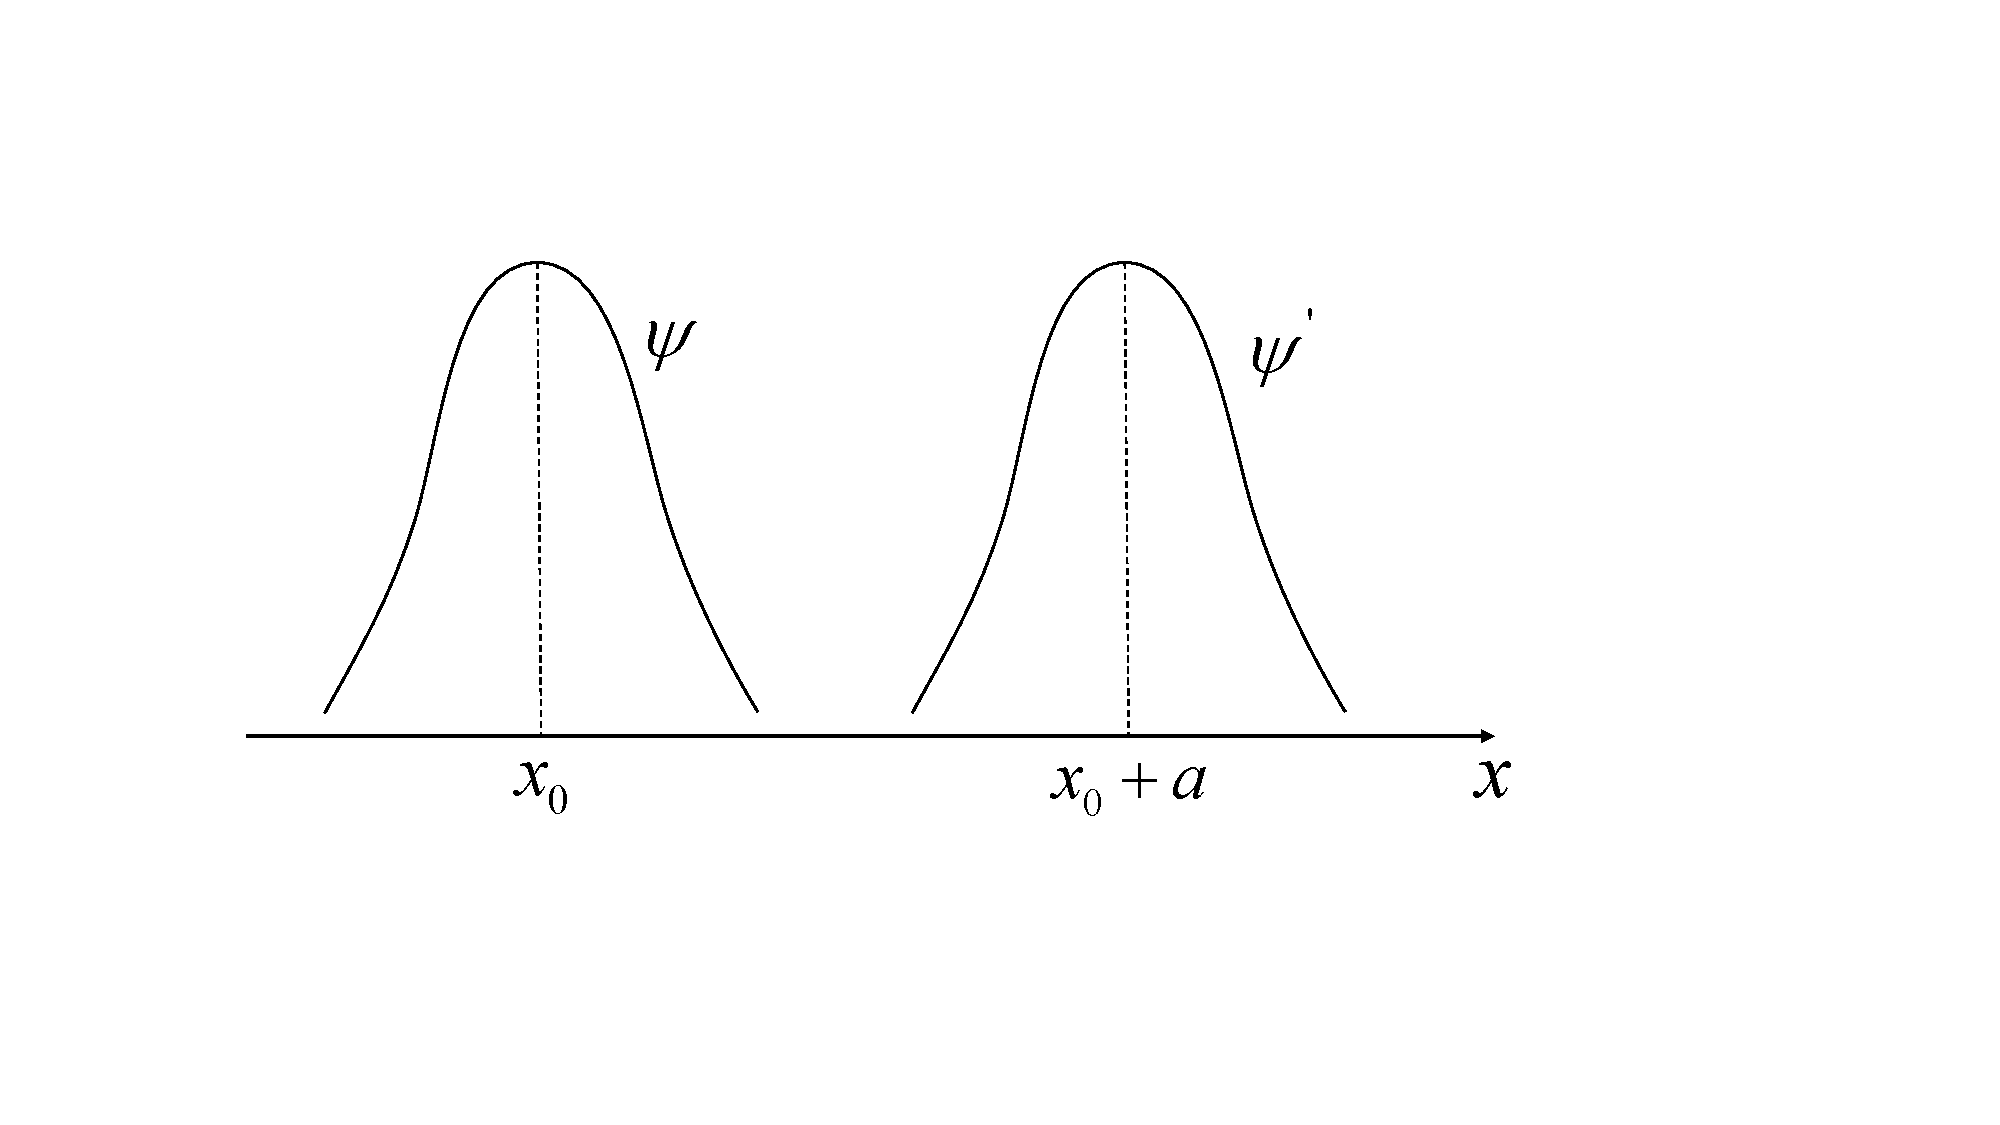
\includegraphics[width=3.5cm,clip]{QM file/figure/3-4}
	\caption{}\label{fig.3-4}
\end{wrapfigure}
\begin{empheq}{equation*}
	\varPsi^{\prime}(x)=\hat{D}(a)\varPsi(x)
\end{empheq}
显然
\begin{empheq}{equation*}
	\varPsi^{\prime}(x+a)=\varPsi(x)
\end{empheq}
因此
\begin{empheq}{equation}\label{eq310.11}
	\varPsi^{\prime}(x)=\hat{D}(a)\varPsi(x)=\varPsi(x-a)
\end{empheq}
这就是平移算符$\hat{D}(a)$对波函数的作用规则.平移显然是一种连续变换.我们先来确定无穷小平移$(a=\delta x\rightarrow 0)$算符$\hat{D}(\delta x)$)的具体形式.按照定义\eqref{eq310.11}式,应有
\eqindent{6}
\begin{empheq}{align*}
	\hat{D}(\delta x)\varPsi(x)&=\varPsi(x-\delta x)	\\
	&=\varPsi(x)-\frac{\partial \varPsi}{\partial x}\delta x=\bigg(1-\delta x\frac{\partial}{\partial x}\bigg)\varPsi(x)
\end{empheq}
所以
\begin{empheq}{align}\label{eq310.12}
	\hat{D}(\delta x)&=1-\delta x\frac{\partial}{\partial x}=1+\delta x\frac{\hat{p}_{x}}{i\hbar}	\nonumber\\
	&=\exp\bigg(\delta x\frac{\hat{p}_{x}}{i\hbar}\bigg)\quad(\delta x\rightarrow 0)
\end{empheq}
其中$\hat{p}_{x}$是动量算符.平移有限距离$a$时,算符$\hat{D}(a)$显然可以表示成
\begin{empheq}{equation}\label{eq310.13}
	\hat{D}(a)=\exp\bigg(-a\frac{\partial}{\partial x}\bigg)=\exp\bigg(a\hat{p}_{x}{i\hbar}\bigg)
\end{empheq}\eqnormal
将其代入\eqref{eq310.11}式,即得
\begin{empheq}{align*}
	\varPsi(x-a)=\exp\bigg(-a\frac{\partial}{\partial x}\bigg)\varPsi(x)	\\
	\sum_{n=0}^{\infty}\frac{(-a)^{n}}{n!}\bigg(\frac{\partial}{\partial x}\bigg)^{n}\varPsi(x)
\end{empheq}
这正是$\varPsi(x-a)$的泰勒(Taylor)展开式.

由以上分析,可知平移确是一种么正变换,满足
\eqindent{6}
\begin{equation}\label{eq310.14}
	\hat{D}^{+}(a)=\exp\bigg(\frac{ia}{\hbar}\hat{p}_{x}\bigg)=\hat{D}^{-1}(a)=\hat{D}(-a)
\end{equation}\eqnormal
其无穷小算子就是动量算符$\hat{p}_{x}$.

如体系的总能量算符$\hat{H}$具有平移不变性,满足
\begin{equation}\label{eq310.15}
	\hat{D}(a)\hat{H}=\hat{H}\hat{D}(a)
\end{equation}
则$\hat{H}$必与$\hat{p}_{x}$对易,即
\begin{empheq}{equation}\label{eq310.16}
	[\hat{p}_{x},\hat{H}]=\hat{p}_{x}\hat{H}-\hat{H}\hat{p}_{x}=0
\end{empheq}
$\hat{p}_{x}$为守恒量,这就是动量守恒定律.对于$\hat{H}$取
\begin{empheq}{equation*}
	\hat{H}=\hat{T}+\hat{V}=-\frac{\hbar^{2}}{2m}\frac{\partial^{2}}{\partial x^{2}}+V(x)
\end{empheq}
的情形,平移不变性要求$[V,p_{x}]$,则
\begin{empheq}{equation*}
	\frac{\partial V}{\partial x}=0,\quad V(x)=c\text{(常量)}
\end{empheq}
在这条件下,体系的动量守恒.经典力学也有同样的结论.

推广到三维问题,对于无限小平移$\delta r=(\delta x,\delta y,\delta z)$,相应的平移算符记为$\hat{D}(\delta \boldsymbol{r})$,应该有
\eqindent{6}
\begin{empheq}{align*}
	\hat{D}(\delta \boldsymbol{r})\varPsi(\boldsymbol{r})&=\varPsi(\boldsymbol{r}-\delta\boldsymbol{r})	\\
	&=\varPsi(\boldsymbol{r})-\bigg(\frac{\partial\varPsi}{\partial x}\delta x+\frac{\partial\varPsi}{\partial y}\delta y+\frac{\partial\varPsi}{\partial z}\delta z\bigg)	\\
	&=\varPsi(\boldsymbol{r})\sim\delta\boldsymbol{r}\cdot\nabla\varPsi
\end{empheq}
所以
\begin{empheq}{align}\label{eq310.17}
	\hat{D}(\delta \boldsymbol{r})&=1-\delta \boldsymbol{r}\cdot\nabla=\exp(-\delta \boldsymbol{r}\cdot\nabla)	\nonumber\\
	&=\exp\bigg(\delta \boldsymbol{r}\cdot\frac{\hat{\boldsymbol{p}}}{i\hbar}\bigg)(\delta \boldsymbol{r}\rightarrow 0)
\end{empheq}\eqnormal
其中$\hat{p}=-i\hbar\nabla$为动量算符.

平移有限距离$\boldsymbol{a}$时,算符$\hat{D}(\boldsymbol{a})$可以表示成
\begin{empheq}{equation}\label{eq310.18}
	\hat{D}(\boldsymbol{a})=\exp(-\boldsymbol{a}\cdot\nabla)=\exp\bigg(\boldsymbol{a}\cdot\frac{\hat{\boldsymbol{p}}}{i\hbar}\bigg)
\end{empheq}
如体系总能量算符$\hat{H}$具有平移不变性,满足
\begin{empheq}{equation}\label{eq310.19}
	\hat{D}(\boldsymbol{a})\hat{H}=\hat{H}\hat{D}(\boldsymbol{a})
\end{empheq}
则$\boldsymbol{a}\cdot\hat{\boldsymbol{p}}=a\hat{p}_{a}$必与$\hat{H}$对易,$\hat{p}_{a}$为守恒量.如上式对任意$\boldsymbol{a}$成立,则
\eqindent{6}
\begin{empheq}{equation}\label{eq310.20}
	[\hat{p}_{\alpha},\hat{H}]=\hat{p}_{\alpha}\hat{H}-\hat{H}\hat{p}_{\alpha}=0,\quad\alpha=x,y,z
\end{empheq}\eqnormal
$\boldsymbol{p}$为守恒量,这就是动量守恒定律.$\hat{H}$取\eqref{eq310.10}式时,平移不变性要求$[V,\hat{p}_{\alpha}]=0(\alpha=x,y,z)$,则
\begin{empheq}{equation*}
	\frac{\partial V}{\partial x},\frac{\partial V}{\partial y}=0,\frac{\partial V}{\partial z}=0,V(\boldsymbol{r})=c\text{(常量)}
\end{empheq}
在这条件下,体系的动量守恒.

{\heiti 3. 旋转不变性和角动量守恒定律}

考虑体系绕任意轴$\boldsymbol{e}_{n}$的旋转,对于无穷小旋转角$\delta\varphi$,相应的转动算符记为$\hat{R}(\delta\varphi)$,$\delta\varphi=\boldsymbol{e}_{n}\delta\varphi$.体系的任何一个状态$\varPsi$,经无限小转动后,变成$\varPsi^{\prime}$,即$\hat{R}(\delta\varphi)\varPsi$,它与$\varPsi$的关系可以仿照平移变换而确定.先考虑一种简单情形,即转轴为球坐标系极轴($z$轴)的情形.令$\hat{R}(\delta\varphi)\varPsi=\varPsi^{\prime}$,显然有
\eqindent{4}
\begin{empheq}{align*}
	\varPsi^{\prime}(r,\theta,\varphi)&=\hat{R}(\delta\varphi)\varPsi(r,\theta,\varphi)=\varPsi(r,\theta,\varphi-\delta\varphi)	\\
	&=\varPsi(r,\theta,\varphi)-\frac{\partial\varPsi}{\partial\varphi}\delta\varphi=\bigg(1-\delta\varphi\frac{\partial}{\partial\varphi}\bigg)\varPsi(r,\theta,\varphi)
\end{empheq}\eqnormal

\begin{wrapfigure}[14]{r}{5em}
	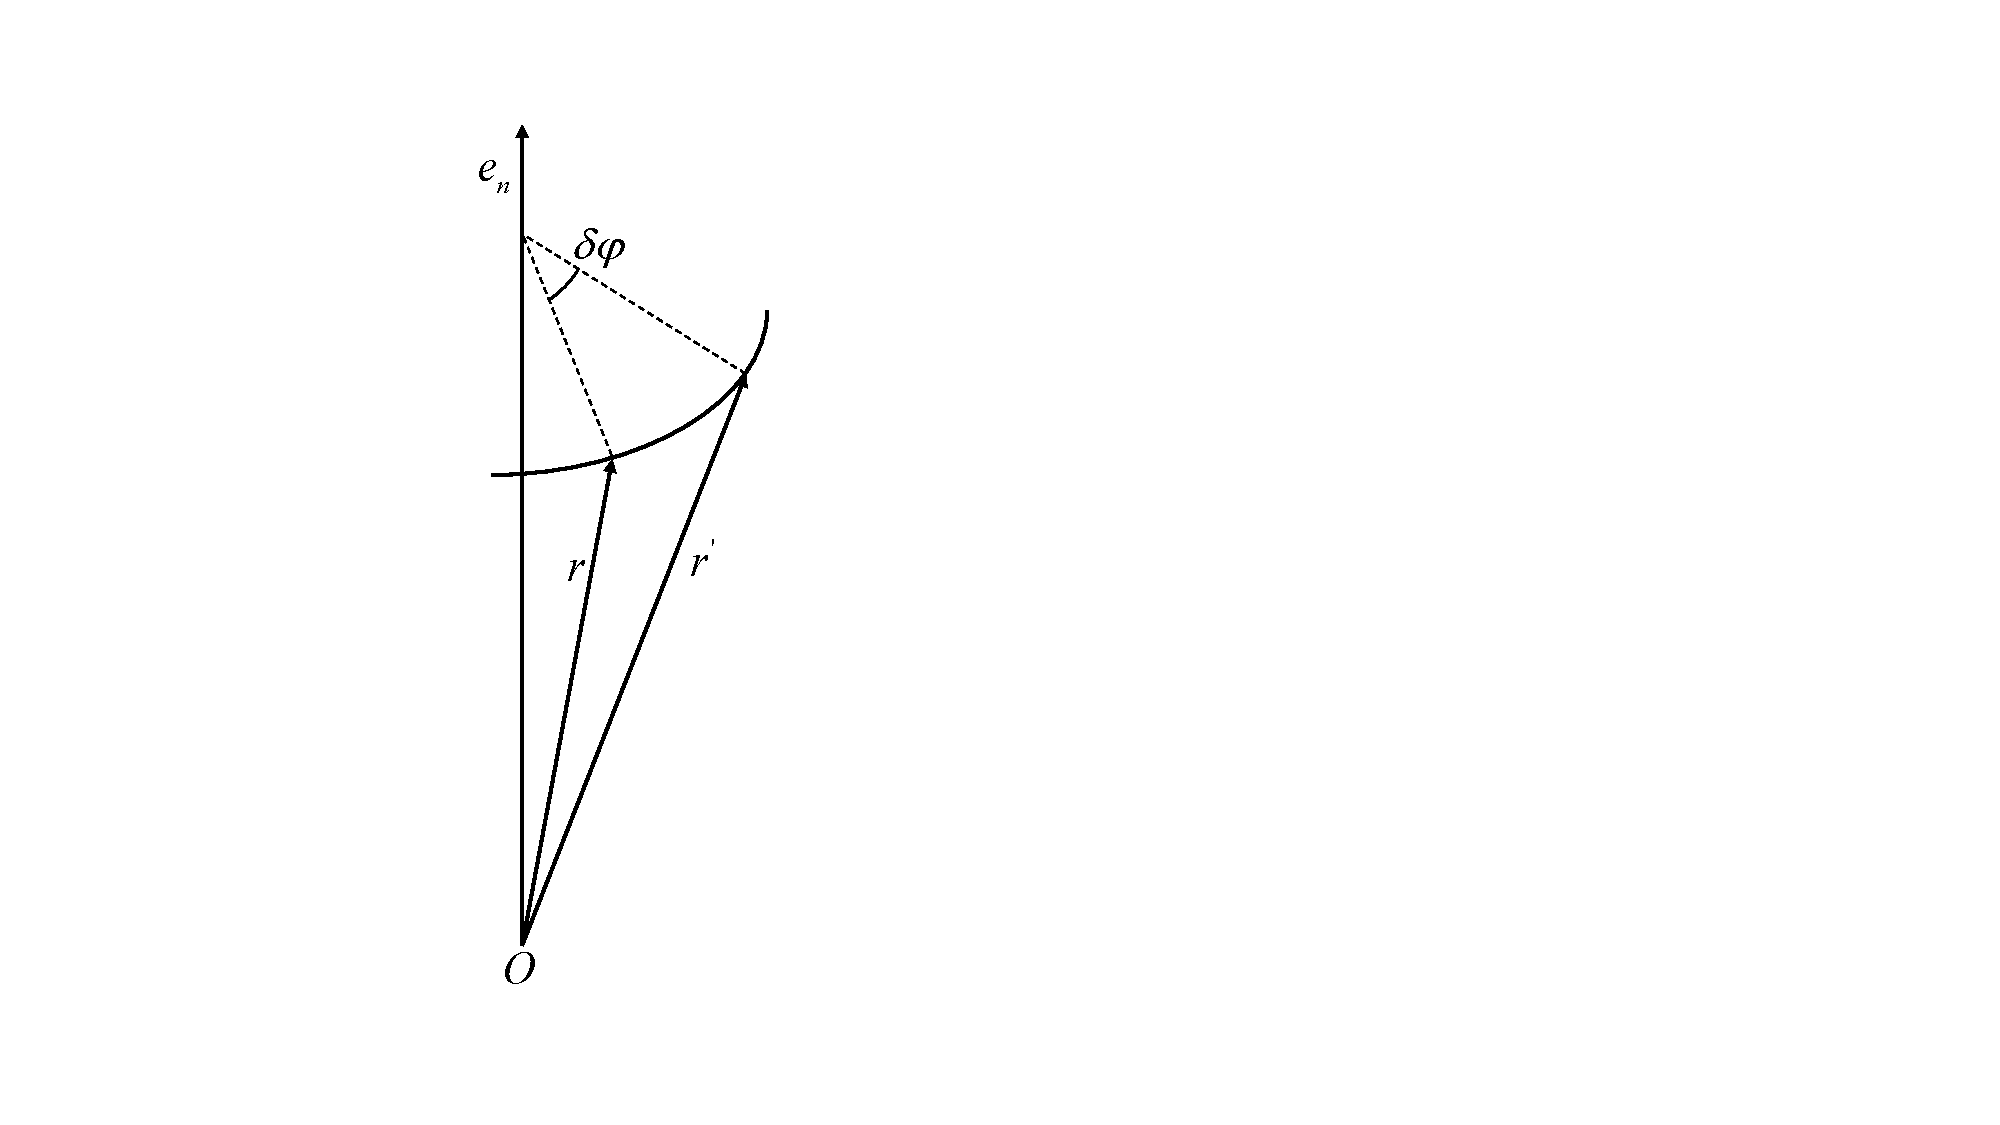
\includegraphics[width=2cm,clip]{QM file/figure/3-5}
	\caption{}\label{fig.3-5}
\end{wrapfigure}
所以
\eqindent{4}
\begin{empheq}{align}\label{eq310.21}
	\hat{R}(\delta\varphi)&=1-\delta\varphi\frac{\partial}{\partial\varphi}=1+\delta\varphi\frac{\hat{L}_{z}}{i\hbar}	\nonumber\\
	&=\exp\bigg(\delta\varphi\frac{\hat{L}_{z}}{i\hbar}\bigg)
\end{empheq}\eqnormal
其中
\eqindent{6}
\begin{empheq}{equation}\label{eq310.22}
	\hat{L}_{z}=-i\hbar\frac{\partial}{\partial\varphi}
\end{empheq}
为转动变换的无穷小算子,这就是轨道角动量($z$分量)算符.

当旋转轴$\boldsymbol{e}_{n}$沿任意方向时,矢径$\boldsymbol{r}$经过无穷小转动后变成(图\ref{fig.3-5})
\begin{empheq}{equation}\label{eq310.23}
	\boldsymbol{r}^{\prime}=\boldsymbol{r}+\delta\boldsymbol{r},\quad\delta\boldsymbol{r}=\delta\varphi\boldsymbol{e}_{n}\times\boldsymbol{r}
\end{empheq}
转动前后波函数关系为
\begin{empheq}{equation}\label{eq310.24}
	\varPsi^{\prime}(\boldsymbol{r}^{\prime})=\varPsi(\boldsymbol{r})
\end{empheq}
\begin{empheq}{align*}
	\varPsi^{\prime}(\boldsymbol{r})&=\hat{R}(\delta\varphi)\varPsi(\boldsymbol{r})=\varPsi(\boldsymbol{r}-\delta\boldsymbol{r})	\\
	&=\varPsi(\boldsymbol{r})-\delta\boldsymbol{r}\cdot\nabla\varPsi(\boldsymbol{r})=(1-\delta\boldsymbol{r}\cdot\nabla)\varPsi(\boldsymbol{r})	\\
	&=[1-\delta\varphi(\boldsymbol{e}_{n}\times\boldsymbol{r})\cdot\nabla]\varPsi(\boldsymbol{r})	\\
	&=[1-\delta\varphi\boldsymbol{e}_{n}\cdot(\boldsymbol{r}\times\nabla)]\varPsi(\boldsymbol{r})
\end{empheq}
所以
\begin{empheq}{align}\label{eq310.25}
	\hat{R}(\delta\varphi)&=1-\delta\varphi\boldsymbol{e}_{n}\cdot(\boldsymbol{r}\times\nabla)	\nonumber\\
	&=1+\frac{\delta\varphi}{i\hbar}\boldsymbol{e}_{n}\cdot\hat{\boldsymbol{L}}
	=\exp\bigg(\frac{\delta\varphi}{i\hbar}\boldsymbol{e}_{n}\cdot\hat{\boldsymbol{L}}\bigg)
\end{empheq}\eqnormal
其中
\begin{empheq}{equation}\label{eq310.26}
	\hat{\boldsymbol{L}}=-i\hbar\boldsymbol{r}\times\nabla=\boldsymbol{r}\times\hat{\boldsymbol{p}}
\end{empheq}
是轨道角动量算符,$\boldsymbol{e}_{n}\cdot\hat{\boldsymbol{L}}=\hat{L}_{n}$是转动变换的无穷小算子.

如体系具有对$\boldsymbol{e}_{n}$轴的旋转不变性,满足
\begin{empheq}{equation}\label{eq310.27}
	\hat{R}(\delta\varphi)\hat{H}=\hat{H}\hat{R}(\delta\varphi)
\end{empheq}
则$\hat{L}_{n}$与$\hat{H}$必然对易,即
\begin{empheq}{equation}\label{eq310.28}
	[\hat{L}_{n},\hat{H}]=\hat{L}_{n}\hat{H}-\hat{H}\hat{L}_{n}=0
\end{empheq}
$L_{n}$为守恒量.如$\hat{H}$具有对任意轴的旋转不变性,则$\hat{\boldsymbol{L}}$各分量均与$\hat{H}$对易,即
\begin{empheq}{equation}\label{eq310.29}
	[\hat{L}_{\alpha},\hat{H}]=\hat{L}_{\alpha}\hat{H}-\hat{H}\hat{L}_{\alpha}=0,\quad\alpha=x,y,z
\end{empheq}
$\boldsymbol{L}$为守恒量.在$\hat{H}$可以表示成\eqref{eq310.10}式的情形下,动能算符$\hat{T}=-\frac{\hbar^{2}}{2m}\nabla^{2}$具有对任意轴的旋转不变性,满足
\begin{empheq}{equation}\label{eq310.30}
	[\hat{L}_{\alpha},\hat{T}]=0,\quad\alpha=x,y,z
\end{empheq}
因此势能$V(r)$具有哪种旋转对称性,$\hat{H}$也具有同样的对称性.例如中心力场,$V=V(r)$,满足
\begin{empheq}{equation}\label{eq310.31}
	[\hat{L}_{\alpha},V(r)]=0,\quad\alpha=x,y,z
\end{empheq}
$V(r)$各向同性,具有对任意轴的旋转不变性,$\hat{H}$也一样,因此$\boldsymbol{L}$为守恒量,这就是角动量守恒定律.

{\heiti 4. 时间平移不变性和能量守恒定律}

在$\S$中\ref{sec:03.09}已经讲过,如体系的哈密顿算符$\hat{H}$不显含$t$,$\hat{H}$就是守恒量,这就是能量守恒定律.$\hat{H}$不显含$t$,意味着体系具有时间均匀性,体系能量不随时间变化,$\frac{\partial\hat{H}}{\partial t}$.当然,在量子力学中,时间$t$并不作为力学量对待,但是我们仍然可以仿照空间平移的概念,引入时间平移概念.任何状态$\varPsi(\boldsymbol{r},t)$的无穷小时间$(\delta t)$平移态记为$D_{t}(\delta t)\varPsi$,它在$t$时刻的情况与$\varPsi$态$(t+\delta t)$时刻的情况相同,即
\begin{empheq}{equation}\label{eq310.32}
	D_{t}(\delta t)\varPsi(\boldsymbol{r},t)=\varPsi(\boldsymbol{r},t+\delta t)
\end{empheq}
由于
\begin{empheq}{equation*}
	\varPsi(\boldsymbol{r},t+\delta t)=\varPsi(\boldsymbol{r},t)+\delta t\frac{\partial}{\partial t}\varPsi(\boldsymbol{r},t)
\end{empheq}
所以无穷小时间平移算符为
\begin{empheq}{equation}\label{eq310.33}
	D_{t}(\delta t)=1+\delta t\frac{\partial}{\partial t}=\exp\bigg(\delta t\frac{\partial}{\partial t}\bigg)
\end{empheq}
有限时间$(\tau)$平移算符为
\begin{empheq}{equation}\label{eq310.34}
	D_{t}(\tau)=\exp\bigg(\tau\frac{\partial}{\partial t}\bigg)
\end{empheq}
任何真实的运动状态$\varPsi(\boldsymbol{r},t)$应该满足薛定谔方程\eqref{eq310.1}式,$\frac{\partial}{\partial t}$对波函数的作用效果等价于$\frac{\hat{H}}{i\hbar}$,所以在时间平移算符中,可作如下等价代换:
\begin{empheq}{equation}\label{eq310.35}
	i\hbar\frac{\partial}{\partial t}\Longrightarrow\hat{H}
\end{empheq}
\begin{empheq}{equation}\label{eq310.36}
	D_{t}(\tau)\Longrightarrow\exp\bigg(\frac{\tau\hat{H}}{i\hbar}\bigg)
\end{empheq}
\eqref{eq310.35}式的含义正是$\S$\ref{sec:02.01}就已经讲过的,$i\hbar\frac{\partial}{\partial t}$代表能量.而\eqref{eq310.36}式表明,时间平移算符等价于演化算符[参看\eqref{eq39.7}式].

体系在时间上的均匀性也称时间平移不变性,这种对称性导致能量守恒定律成立.但应注意,这并不意味若体系在任何时刻必定处于能量本征态.这里“能量守恒”的确切内容是体系的能量平均值以及各个能量本征值的测量概率不随时间改变.以$\varPsi(\boldsymbol{r})$表示$\hat{H}$的本征态,本征值记为$E_{n}$.如在初始时刻$(t_{0}=0)$体系处于能量本征态$\varPsi_{n}$,波函数的时间演化规律为
\begin{empheq}{equation}\label{eq310.37}
	\varPsi_{n}(\boldsymbol{r},t)=\varPsi_{n}(\boldsymbol{r})e^{-E_{n}t/i\hbar}
\end{empheq}
这就是定态波函数.上式的时间平移$(\tau)$态为
\eqindent{6}
\begin{empheq}{align}\label{eq310.38}
	D_{t}\varPsi_{n}(\boldsymbol{r},t)&=e^{\tau\frac{\partial}{\partial t}}\varPsi_{n}(\boldsymbol{r})e^{-iE_{n}t/\hbar}	\nonumber\\
	&=\varPsi_{n}(\boldsymbol{r})\exp\bigg[-\frac{i}{\hbar}E_{n}(t+\tau)\bigg]
\end{empheq}\eqnormal
仍是原来的定态,只是添了相因子$\exp\bigg(-\frac{i}{\hbar}E_{n}(t+\tau)\bigg)$.如初始状态不是单一的能量本征态,则总可以表示成各$\varPsi_{n}$的线性叠加:
\begin{empheq}{equation}\label{eq310.39}
	\varPsi(\boldsymbol{r},t)=\sum_{n}C_{n}\varPsi_{n}(\boldsymbol{r})
\end{empheq}
波函数的时间演化规律为[\eqref{eq39.6}式]
\begin{empheq}{align}\label{eq310.40}
	\varPsi(\boldsymbol{r},0)&=\exp\bigg(\frac{\hat{H}t}{i\hbar}\bigg)\varPsi(\boldsymbol{r},0)	\nonumber\\
	&=\sum_{n}C_{n}\varPsi_{n}(\boldsymbol{r})e^{-E_{n}t/\hbar}
\end{empheq}
上式的时间平移$(\tau)$态为
\eqindent{6}
\begin{empheq}{align}\label{eq310.41}
	D_{t}(\tau)\varPsi(\boldsymbol{r},t)&=\exp\bigg(\frac{\hat{H}\tau}{i\hbar}\bigg)\varPsi(\boldsymbol{r},t)	\nonumber\\
	&=\exp\bigg[\frac{\hat{H}(t+\tau)}{i\hbar}\bigg]\varPsi(\boldsymbol{r},0)	\nonumber\\
	&=\sum_{n}C_{n}\varPsi_{n}(\boldsymbol{r})\exp\bigg[-\frac{i}{\hbar}E_{n}(t+\tau)\bigg]	\nonumber\\
	&=\varPsi(\boldsymbol{r},t+\tau)
\end{empheq}\eqnormal
显然,无论是\eqref{eq310.40}式还是\eqref{eq310.41}式,能量本征值$E_{n}$的测量概率均为$|C_{n}|^{2}$,与时间$t$及$\tau$无关,而仅取决于初始状态$\varPsi(\boldsymbol{r},0)$.

\example 质量为$m$的粒子作三维运动,已知总能量算符为
\begin{empheq}{equation}\label{eq310.42}
	\hat{H}=\hat{T}+V=-\frac{\hbar^{2}}{2m}\nabla^{2}+\frac{k}{2}(x^{2}+y^{2})
\end{empheq}
试分析其对称性并找出相应的守恒量.

\solution 首先,$\hat{H}$不显含$t$,具有时间均匀性,$H$为守恒量(能量守恒).$H_{x}=\frac{p_{x}^{2}}{2m}+\frac{kx^{2}}{2}$,$H_{y}=\frac{p_{y}^{2}}{2m}+\frac{ky^{2}}{2}$和$H_{z}=\frac{p_{z}^{2}}{2m}+\frac{kz^{2}}{2}$也都是守恒量.

其次,$\hat{H}$显然具有空间反射不变性,所以宇称守恒.

由于势能$V$与$z$无关,$\hat{H}$具有$z$方向平移不变性,所以动量的$z$分量$p_{z}$是守恒量.

势能$V$还具有绕$z$轴的旋转不变性,$\frac{\partial V}{\partial\varphi}$,所以轨道角动盘的$z$分量$L_{z}$,也是守恒量.








% 海尔曼定理和位力定理
\section[海尔曼定理和位力定理]{海尔曼定理和位力定理} \label{sec:03.11} % 
% \makebox[5em][s]{} % 短题目拉间距

关于物理体系的能量本征态(束缚态),有许多定理,其中最重要、应用最广的大概就是海尔曼(H.Hellmann)定理和位力(Virial) 定理了.海尔曼定理发表于20世纪30年代后期,最初是用来讨论量子化学问题的,因此在量子力学教科书中较少提到它.其实这个定理应用极广.
\newpage
{\heiti 1. 海尔曼定理}

设某个体系的束缚态能级和归一化能量本征函数为$E_{n}$,$\varPsi_{n}$($n$代表全体量子数或本征态编号数),满足能量本征方程
\begin{empheq}{equation}\label{eq311.1}
	\hat{H}\varPsi_{n}-E_{n}\varPsi_{n}=0
\end{empheq}
设$\lambda$为$\hat{H}$中含有的任何一个参数(如粒子质量$m$,普朗克常数$\hbar$,等等),显然$E_{n}$,$\varPsi_{n}$均与$\lambda$有关.\eqref{eq311.1}式对$\lambda$求导,得到
\begin{empheq}{equation*}
	\bigg(\frac{\partial\hat{H}}{\partial\lambda}-\frac{\partial E_{n}}{\partial \lambda}\bigg)\varPsi_{n}+(\hat{H}-E_{n})\frac{\partial\varPsi_{n}}{\partial\lambda}=0
\end{empheq}
左乘$\varPsi^{*}$,对全空间积分,得到
\eqindent{6}
\begin{empheq}{align}\label{eq311.2}
	\int\varPsi^{*}(\hat{H}-E_{n})\frac{\partial\varPsi_{n}}{\partial\lambda}d\tau
	&=\int\varPsi_{n}^{*}\bigg(\frac{\partial E_{n}}{\partial\lambda}-\frac{\partial\hat{H}}{\partial\lambda}\bigg)\varPsi_{n}d\tau	\nonumber\\
	&=\frac{\partial E_{n}}{\partial \lambda}-\bigg\langle\frac{\partial\hat{H}}{\partial\lambda}\bigg\rangle_{n}
\end{empheq}
其中$\langle\rangle_{n}$表示$\varPsi_{n}$态下的平均值.由于$\hat{H}=\hat{H}^{+}$,上式左端与$\hat{H}$有关的积分即
\begin{empheq}{align*}
	\int\varPsi^{*}\hat{H}\frac{\partial\varPsi_{n}}{\partial\lambda}d\tau
	&=\int\frac{\partial\varPsi_{n}}{\partial\lambda}(\hat{H}\varPsi_{n})^{*}d\tau	\\
	&=E_{n}\int\frac{\partial\varPsi_{n}}{\partial\lambda}\varPsi_{n}^{*}d\tau
\end{empheq}\eqnormal
因此\eqref{eq311.2}式左端等于0,于是得到
\begin{empheq}{equation}\label{eq311.3}
	\boxed{\frac{\partial E_{n}}{\partial\lambda}=\bigg\langle\frac{\partial\hat{H}}{\partial\lambda}\bigg\rangle_{n}\equiv\int\varPsi_{n}^{*}\frac{\partial\hat{H}}{\partial\lambda}\varPsi_{n}d\tau}
\end{empheq}
\eqref{eq311.3}式称为海尔曼定理或海尔曼公式.

适当地选择参数$\lambda$,$\frac{\partial\hat{H}}{\partial\lambda}$常常可以表示某些重要的力学量算符,所以利用海尔曼定理常可求出某些重要力学量的平均值,或求出能级.海尔曼定理也常用作理论分析的工具,例如用它来证明其他定理,下面先证明一个定理.

\theorem 粒子在势场$V_{1}(x)$中运动时,束缚态能级为$E_{n}(1)$;在势场$V_{2}(x)$中运动时,束缚态能级为$E_{n}(2)$.其中$n=1,2,3,\cdots$为能级编号.设对于任何$x$值,均有$V_{1}(x)\leqslant V_{2}(x)$,则
\begin{empheq}{equation*}
	E_{n}(1)\leqslant E_{n}(2)
\end{empheq}

\prove 考虑另一个介乎$V_{1},V_{2}$之间的势场
\eqindent{5}
\begin{empheq}{equation}\label{eq311.4}
	V(\lambda,x)=(2-\lambda)V_{1}(x)+(\lambda-1)V_{2}(x),\quad 1\leqslant \lambda\leqslant 2
\end{empheq}\eqnormal
当$\lambda=1,2,$上式即$V_{1}(x),V_{2}(x)$.粒子在势场$V(\lambda,x)$中运动时,总能量算符为
\begin{empheq}{equation}\label{eq311.5}
	\hat{H}(\lambda,x)=-\frac{\hbar^{2}}{2m}\frac{d^{2}}{dx^{2}}+V(\lambda,x)
\end{empheq}
相应的束缚态能级记为$E_{n}(\lambda)$,$n=1,2,3,\cdots$.\eqref{eq311.1}式对$\lambda$求导,得到
\begin{empheq}{equation*}
	\frac{\partial\hat{H}}{\partial\lambda}=\frac{\partial V(\lambda,x)}{\partial\lambda}=V_{2}(x)-V_{1}(x)\geqslant 0
\end{empheq}
由海尔曼定理,即得
\begin{empheq}{equation*}
	\frac{\partial}{\partial\lambda}E_{n}(\lambda)=\langle V_{2}-V_{1} \rangle_{n}\geqslant 0
\end{empheq}
这表明$\lambda$增加时$E_{n}(\lambda)$只增不减,所以$E_{n}(1)\geqslant E_{n}(2)$.

这个定理常用来对不同势场所造成的能级作定性比较分析.

\exa 已知一维谐振子的总能量算符和能级为
\begin{empheq}{equation}\label{eq311.6}
	\hat{H}=\hat{T}+V=-\frac{h^{2}}{2m}\frac{d^{2}}{dx^{2}}+\frac{1}{2}m\omega^{2}x^{2}
\end{empheq}
\begin{empheq}{equation}\label{eq311.7}
	E_{n}=\bigg(n+\frac{1}{2}\bigg)\hbar\omega,\quad n=0,1,2,\cdots
\end{empheq}

试用海尔曼定理证明,在能量本征态$\varPsi_{n}$下,
\begin{empheq}{equation}\label{eq311.8}
	\bar{T}=\bar{V}=\frac{1}{2}E_{n}
\end{empheq}

\prove 总能量算符$\hat{H}$中含有三个参数$\hbar$,$m$,$\omega$,其中任何一个均可取作海尔曼定理\eqref{eq311.3}式中的$\lambda$.如取$\lambda=\hbar$,
\begin{empheq}{equation*}
	\frac{\partial\hat{H}}{\partial\lambda}=-\frac{\hbar}{m}\frac{d^{2}}{dx^{2}}=\frac{2}{\hbar}\hat{T}
\end{empheq}
按照\eqref{eq311.3}式,就有
\begin{empheq}{equation*}
	\frac{\hbar}{\hbar}\langle T \rangle_{n}=\frac{\partial E_{n}}{\partial\hbar}=\bigg(n+\frac{1}{2}\bigg)\omega=\frac{E_{n}}{\hbar}
\end{empheq}
所以
\begin{empheq}{equation*}\label{eq311.8'}
	\langle T \rangle_{n}=\frac{1}{2}E_{n}	\tag{$3.11.8^{\prime}$}
\end{empheq}
由于
\begin{empheq}{equation*}
	E_{n}=\langle T+V \rangle_{n}
\end{empheq}
所以
\begin{empheq}{equation*}\label{eq311.8''}
	\langle V \rangle_{n}=E_{n}-\langle T \rangle_{n}=\frac{1}{2}E_{n}	\tag{$3.11.8^{\prime\prime}$}
\end{empheq}
如取$\lambda=m$或$\omega$,同样可以证明\eqref{eq311.8}式,读者试自完成之.

\exa 质量$m$,电荷$q$的粒子,受到弹性力$(-kx)$和均匀电场$\mathscr{E}$(指向正$x$轴方向)的共同作用,势能可以表示成
\begin{empheq}{equation}\label{eq311.9}
	V(x)=\frac{1}{2}kx^{2}-q\mathscr{E}x
\end{empheq}

求束缚能级.

\solution 总能量算符为
\begin{empheq}{equation}\label{eq311.10}
	\hat{H}=\hat{T}+V=-\frac{\hbar^{2}}{2m}\frac{d^{2}}{dx^{2}}+\frac{1}{2}kx^{2}-q\mathscr{E}x
\end{empheq}
视电场强度$\mathscr{E}$为参数,设能级为$E_{n}(\mathscr{E})$.当$\mathscr{E}=0$,\eqref{eq311.10}式即谐振子能量算符,其本征值为
\begin{empheq}{equation}\label{eq311.11}
	E_{n}(0)=\bigg(n+\frac{1}{2}\bigg)\hbar\omega,\quad\omega=\sqrt{\frac{k}{m}}
\end{empheq}
\eqref{eq311.10}式对$\mathscr{E}$求导,得到$\frac{\partial\hat{H}}{\partial\mathscr{E}}=-qx$,再利用海尔曼定理,即得
\begin{empheq}{equation}\label{eq311.12}
	\frac{\partial}{\partial\mathscr{E}}E_{n}(\mathscr{E})=-q\langle x \rangle_{n}
\end{empheq}
另一方面,
\begin{empheq}{align}\label{eq311.13}
	[\hat{p}_{x},\hat{H}]&=\frac{k}{2}[\hat{p}_{x},x^{2}]-q\mathscr{E}[\hat{p}_{x},x]	\nonumber\\
	&=-i\hbar(kx-q\mathscr{E})
\end{empheq}
上式在$\varPsi_{n}$态下求平均,由于
\begin{empheq}{equation*}
	[p_{x},H]=\int\varPsi_{n}^{*}(\hat{p}_{x}\hat{H}-\hat{H\hat{p}_{x}})\varPsi_{n}dx=0
\end{empheq}
(请读者自己证明)故得
\begin{empheq}{equation}\label{eq311.14}
	\langle x \rangle_{n}=\frac{q\mathscr{E}}{k}=\frac{q\mathscr{E}}{m\omega^{2}}
\end{empheq}
代入\eqref{eq311.12}式,得到
\begin{empheq}{equation*}\label{eq311.12'}
	\frac{\partial}{\partial\mathscr{E}}E_{n}(\mathscr{E})=-\frac{q^{2}\mathscr{E}}{k}	\tag{$3.11.12^{\prime}$}
\end{empheq}
积分,即得
\eqindent{5}
\begin{empheq}{gather}\label{eq311.15}
	E_{n}(\mathscr{E})=E_{n}(0)-\frac{q^{2}\mathscr{E}^{2}}{2k}=\bigg(n+\frac{1}{2}\bigg)\hbar\omega-\frac{q^{2}\mathscr{E}^{2}}{2m\omega^{2}}	\\ 
	\qquad \qquad \qquad n=0,1,2,\cdots	\nonumber
\end{empheq}\eqnormal
这就是所求束缚能级.请将本例和$\S$\ref{sec:02.05}的例题对照比较.
\newpage
{\heiti 2. 位力定理}

在经典力学中,质量为$m$的质点在势场$V(r)$中运动时,运动方程为
\begin{empheq}{equation}\label{eq311.16}
	\boldsymbol{p}=m\frac{d\boldsymbol{r}}{dt},\quad\frac{d\boldsymbol{p}}{dt}=\boldsymbol{F}=-\nabla V
\end{empheq}
因此
\eqindent{6}
\begin{empheq}{equation}\label{eq311.17}
	\frac{d}{dt}(\boldsymbol{r}\cdot\boldsymbol{p})=\frac{d\boldsymbol{r}}{dt}\cdot\boldsymbol{p}+\boldsymbol{r}\cdot\frac{d\boldsymbol{p}}{dt}=\frac{\boldsymbol{p}^{2}}{m}-\boldsymbol{r}\cdot\nabla V
\end{empheq}
如果粒子被局限在有限范图内运动(例如沿闭合轨道作周期运动),$\boldsymbol{r}\cdot\boldsymbol{p}$必取有限值,取\eqref{eq311.17}式的长时间平均(对于周期运动,取周期平均值),左端的平均必然等于0,故得
\begin{empheq}{equation}\label{eq311.18}
	\bigg(\frac{\boldsymbol{p}^{2}}{2m}\bigg)_{\text{平均}}=\frac{1}{2}(\boldsymbol{r}\cdot\nabla)_{\text{平均}}=-\frac{1}{2}(\boldsymbol{r}\cdot\boldsymbol{F})_{\text{平均}}
\end{empheq}
这就是经典力学中的位力定理.由于动能总是正的,所以$\boldsymbol{r}\cdot\boldsymbol{F}$的平均值应该是负的,亦即$\boldsymbol{F}$的性质是以吸引力为主.只有这样才能将粒子限制在有限区域内运动.

在量子力学中,当粒子在势场$V(\boldsymbol{r})$ 中运动时,总能量算符为
\begin{empheq}{equation}\label{eq311.19}
	\hat{H}=\hat{T}+\hat{V}=-\frac{\hbar^{2}}{2m}\nabla^{2}+V(\boldsymbol{r})
\end{empheq}
利用\eqref{eq39.17'},\eqref{eq39.18'},\eqref{eq39.32}式,可以证明算符公式
\begin{empheq}{equation}\label{eq311.20}
	\frac{d}{dt}(\hat{\boldsymbol{r}}\cdot\hat{\boldsymbol{p}})\equiv\frac{1}{i\hbar}[\hat{\boldsymbol{r}}\cdot\hat{\boldsymbol{p}},\hat{H}]=\frac{\hat{\boldsymbol{p}}^{2}}{m}-\boldsymbol{r}\cdot\nabla V
\end{empheq}
上式对任何一个能量本征态(束缚态)$\varPsi_{n}$取平均值,由于
\begin{empheq}{equation*}
	\langle[\hat{\boldsymbol{r}}\cdot\hat{\boldsymbol{p}},\hat{H}]\rangle_{n}
	\equiv\int\varPsi_{n}^{*}(\hat{\boldsymbol{r}}\cdot\hat{\boldsymbol{p}}\hat{H}-\hat{H}\hat{\boldsymbol{r}}\cdot\hat{\boldsymbol{p}})\varPsi_{n}d\tau=0
\end{empheq}\eqnormal
故得
\begin{empheq}{equation}\label{eq311.21}
	\boxed{\langle \frac{\boldsymbol{p}^{2}}{2m} \rangle_{n}=\frac{1}{2}\langle \boldsymbol{r}\cdot\nabla V \rangle_{n}}
\end{empheq}
这就是量子力学中的位力定理,它是经典位力定理的推广.注意\eqref{eq311.18}式的平均是对时间的平均,\eqref{eq311.21}式则是对束缚定态平均.

也可以利用海尔曼定理并结合坐标的尺度变换来证明位力定理,如下.\eqref{eq311.19}式对$\hbar$求导,得到
\begin{empheq}{equation}\label{eq311.22}
	\frac{\partial\hat{H}}{\partial\hbar}=-\frac{\hbar}{m}\nabla^{2}=\frac{2}{\hbar}\frac{\hat{\boldsymbol{p}^{2}}}{2m}
\end{empheq}
再利用海尔曼定理,即得
\begin{empheq}{equation}\label{eq311.23}
	\langle\frac{\hat{\boldsymbol{p}^{2}}}{2m}\rangle_{n}=\frac{\hbar}{2}\frac{\partial E_{n}}{\partial\hbar}
\end{empheq}
另一方面,如作坐标的尺度变换,令
\begin{empheq}{equation}\label{eq311.24}
	\boldsymbol{R}=\frac{\boldsymbol{r}}{\hbar}=(X,Y,Z)
\end{empheq}
则
\eqindent{6}
\begin{empheq}{align*}\label{eq311.19'}
	\hat{H}&=-\frac{1}{2m}\nabla_{R}^{2}+V(\hbar\boldsymbol{R})	\\
	&=-\frac{1}{2m}\bigg(\frac{\partial^{2}}{\partial X^{2}}+\frac{\partial^{2}}{\partial Y^{2}}+\frac{\partial^{2}}{\partial Z^{2}}\bigg)+V(\hbar\boldsymbol{R})
	\tag{$3.11.19^{\prime}$}
\end{empheq}\eqnormal
这时
\begin{empheq}{equation}\label{eq311.25}
	\frac{\partial\hat{H}}{\partial\hbar}=\frac{\partial V}{\partial\hbar}=\frac{\partial\boldsymbol{r}}{\partial\hbar}\cdot\nabla V=\frac{\boldsymbol{r}}{\hbar}\cdot\nabla V(\boldsymbol{r})
\end{empheq}
坐标变换对能级当然没有影响,因此,再利用海尔曼定理,得到
\begin{empheq}{equation}\label{eq311.26}
	\langle \boldsymbol{r}\cdot\nabla V(\boldsymbol{r}) \rangle_{n}=\hbar\frac{\partial E_{n}}{\partial\hbar}
\end{empheq}
比较\eqref{eq311.23}、\eqref{eq311.26}式,即得
\begin{empheq}{equation}\label{eq311.27}
	\langle \frac{\boldsymbol{p}^{2}}{2m} \rangle_{n}=\frac{1}{2}\langle \boldsymbol{r}\cdot\nabla V(\boldsymbol{r}) \rangle_{n}=\frac{\hbar}{2}\frac{\partial E_{n}}{\partial\hbar}
\end{empheq}
其中第一个等式就是位力定理.

位力定理可以推广到多粒子体系.以$x_{\alpha}$($\alpha=1,2,\cdots,3N$,$N$为粒子数)表示各粒子的位置,体系的总动能算符可以表示成
\begin{empheq}{equation}\label{eq311.28}
	\hat{T}=\sum_{\alpha}\frac{1}{2m}\hat{p}_{\alpha}=-\hbar^{2}\sum_{\alpha}\frac{1}{2m_{\alpha}}\bigg(\frac{\partial}{\partial x_{\alpha}}\bigg)^{2}
\end{empheq}
体系的总势能(包括外场作用势和粒子间相互作用势)表示成
\begin{empheq}{equation}\label{eq311.29}
	V=V(x_{1},x_{2},\cdots,x_{\alpha},\cdots,x_{3N})
\end{empheq}
体系的总能量算符为
\begin{empheq}{equation}\label{eq311.30}
	\hat{H}=\hat{T}+V
\end{empheq}
仿照上述步骤,仍有
\begin{empheq}{equation}\label{eq311.31}
	\frac{\partial\hat{H}}{\partial\hbar}=\frac{2}{\hbar}\hat{T}=-2\hbar\sum_{\alpha}\frac{1}{2m}\bigg(\frac{\partial}{\partial x_{\alpha}}\bigg)^{2}
\end{empheq}
作尺度变换
\eqindent{12}
\begin{empheq}{equation}\label{eq311.32}
	X_{\alpha}=\frac{x_{\alpha}}{\hbar}
\end{empheq}\eqnormal
后,则有
\eqindent{4}
\begin{empheq}{equation}\label{eq311.33}
	\frac{\partial\hat{H}}{\partial\hbar}=\frac{\partial V}{\partial\hbar}=\sum_{\alpha}\frac{\partial x_{\alpha}}{\partial\hbar}\frac{\partial V}{\partial x_{\alpha}}=\frac{1}{\hbar}\sum_{\alpha}x_{\alpha}\frac{\partial V}{\partial x_{\alpha}}
\end{empheq}
利用海尔曼定理,得到
\begin{empheq}{equation}\label{eq311.34}
	\langle T \rangle_{n}=\sum_{\alpha}\frac{1}{2m_{\alpha}}\langle p_{\alpha}^{2}\rangle_{n}=\frac{1}{2}\sum_{\alpha}\bigg\langle x_{\alpha}\frac{\partial V}{\partial x_{\alpha}}\bigg\rangle_{n}=\frac{\hbar}{2}\frac{\partial E_{n}}{\partial\hbar}
\end{empheq}\eqnormal
这就是多粒子体系的位力定理.

如果势能$V$是全体$x_{\alpha}$的$\nu$次齐次函数,即
\begin{empheq}{equation}\label{eq311.35}
	V(\lambda x_{1},\lambda x_{2},\cdots)=\lambda^{\nu}V(x_{1},x_{2},\cdots)
\end{empheq}
上式对$\lambda$求导,再取$\lambda=1$,得到
\eqindent{12}
\begin{empheq}{equation}\label{eq311.36}
	\sum_{\alpha}x_{\alpha}\frac{\partial V}{\partial x_{\alpha}}=\nu V
\end{empheq}
对于单粒子体系,就是
\begin{empheq}{equation*}\label{eq311.36'}
	\boldsymbol{r}\cdot\nabla V=\nu V	\tag{$3.11.36^{\prime}$}
\end{empheq}\eqnormal
将\eqref{eq311.36}式代入\eqref{eq311.34}式[\eqref{eq311.36'}式代入\eqref{eq311.27}式],得到
\begin{empheq}{equation}\label{eq311.37}
	\boxed{\langle T \rangle_{n}=\frac{\nu}{2}\langle V \rangle_{n}=\frac{\hbar}{2}\frac{\partial E_{n}}{\partial\hbar}}
\end{empheq}
例如谐振子,$V\propto x^{2}$(或$r^{2}$),相当于$\nu=2$,故有
\begin{empheq}{equation}\label{eq311.38}
	\langle T \rangle_{n}=\langle V \rangle_{n}=\frac{E_{n}}{2}\quad (E_{n}\propto\hbar)
\end{empheq}
又如受反平方吸引力作用的粒子,$V\propto\frac{1}{r}$,相当于$\nu=-1$,所以
\begin{empheq}{equation}\label{eq311.39}
	\langle T \rangle_{n}=-\frac{1}{2}\langle V \rangle_{n}=-E_{n}\quad (E_{n}\propto\hbar^{-2})
\end{empheq}
多电子原子或分子,粒子间作用势为库仑势,相当于$\nu=-1$的情形,所以体系总动能和总势能的束缚定态平均值仍保持\eqref{eq311.39}式的关系.

\exa 粒子在下列势场中运动,

\begin{empheq}{equation}\label{eq311.40}
	V(x)=\lim_{\nu\rightarrow\infty}V_{0}\bigg(\frac{x}{a}\bigg)^{2\nu},a,V_{0}>0
\end{empheq}

讨论势场的性质,并求$T,V$的定态平均值与能级的关系.

\solution 显然当$|x|>a$,$V=\infty$;当$|x|<a$,$V=O$.所以\eqref{eq311.40}式代表宽$2a$的无限深势阱.$V(x)$是$x$的$2\nu(\nu\rightarrow\infty)$次函数,按照\eqref{eq311.37}式,
\begin{empheq}{equation}\label{eq311.41}
	\langle V \rangle_{n}=\frac{1}{\nu}\langle T \rangle_{n}=0,\quad(\nu\rightarrow\infty)
\end{empheq}
因此
\begin{empheq}{equation}\label{eq311.42}
	\langle T \rangle_{n}=E_{n}-\langle V \rangle_{n}=E_{n}
\end{empheq}
请将本题结果和$\S$\ref{sec:02.04}(1.)的结果联系起来理解.









% 习题
\begin{exercises}

\exercise 粒子在一维无限深势阱[$\S$\ref{sec:02.04}(1.)]中运动,已知初始波函数,$\varPsi(x,0)=\frac{1}{\sqrt{2}}[\varPsi_{1}(x)+\varPsi_{2}(x)]$,求$\varPsi(x,t)$,$\bar{E}$,$\overline{E^{2}}$,$\bar{x}(t)$.

\exercise 粒子在一维无限深势阱($0<x<a$,见2-5题)中运动,初始波函数为$\varPsi(x,0)=cx(a-x)$,$c$为归一化常数,请确定$c$,并计算各能量本征值$(E_{n})$的测量概率以及$\bar{E}$,$\Delta E$.

\exercise 已知平面转子(见2-6题)初始波函数为$\varPsi(\varphi,0)=A\sin^{2}\varphi$,$A$为归一化常数,请确定$A$,并求$\varPsi(\varphi,t)$以及$\bar{E}$,$\Delta E$.

\exercise 粒子作一维自由运动,$-\infty<x<\infty$,已知初始波函数为$\varPsi(x,0)=A(\sin^{2}k_{0}x+\cos k_{0}x)$,求$\varPsi(x,t)$,动量$(p_{x})$及动能的取值及概率以及平均值.

\exercise 一维谐振子,初始波函数为$\varPsi(x,0)=\frac{\sqrt{3}}{2}\varPsi_{0}(x)+\frac{1}{2}\varPsi_{1}(x)$,求:$\varPsi(x,t)$,$\bar{E}(t)$,$\bar{x}(t)$,$\bar{p}_{x}(t)$.

\exercise 谐振子处于基态,求动量分布概率,并据此计算动能平均值以及$\Delta p$,与2-14题的结果比较.

\exercise 一维谐振子$\bigg(V=\frac{kx^{2}}{2}\bigg)$处于基态.如势场突然变成$V_{2}(x)=kx^{2}$,即弹性力增大一倍.求$V_{2}$场的能级以及粒子处于新势场中基态的概率.

\exercise 粒子处于一维无限深势阱$(|x|<a)$中的基态.如势阱突然扩展至$|x|<2a$,(阱宽加倍)设扩展时粒子的波函数不变.求扩展后粒子能量的可能测值以及粒子处于新势阱基态的概率.

\exercise 证明:对于任何一维束缚态,$\overline{xp_{x}}=\frac{i\hbar}{2}$,$\overline{p_{x}x}=-\frac{i\hbar}{2}$,并举一个实例验证之.

\exercise 粒子作一维运动,如归一化波函数$\varPsi(x)=u(x)e^{i\hbar x}$,$u(x)$及$k$均为实数,求动量平
均值.

\exercise 利用基本对易式$[x,p_{x}]=i\hbar$等,计算$[p_{x},L_{y}]$,$[p_{x},L_{z}]$,并写出另外几个下标轮换$(x\rightarrow y\rightarrow z\rightarrow x)$公式.

\exercise 证明算符关系:
\begin{empheq}{align*}
	\boldsymbol{r}\times\boldsymbol{L}+\boldsymbol{L}\times\boldsymbol{r}&=2i\hbar\boldsymbol{r}	\\
	\boldsymbol{p}\times\boldsymbol{L}+\boldsymbol{L}\times\boldsymbol{p}&=2i\hbar\boldsymbol{p}
\end{empheq}

\exercise 设线性算符$F$不是厄密的,即$F\neq F^{+}$.试证明$F$可以分解成$F=A+iB$,$A,B$均为厄密算符.求$A,B$.

\exercise 设$U$为么正算符,$(UU^{+}=U^{*}U=1)$证明$U$必可分解成$U=A+iB$,$A,B$为对易$(AB=BA)$厄密算符,而且$A^{2}+B^{2}=1$.进一步再证明$U$可以表示成$U=e^{iD}$的形式,$D$为厄密算符.
[提示:$A,B$的共同本符函数是完备系,本征值$a_{n},b_{n}$.满足关系$a_{n}^{2}+b_{n}^{2}=1$.]

\exercise 算符$A$(无量纲)的指数函数定义成
\begin{empheq}{equation*}
	e^{A}=\sum_{n=0}^{\infty}\frac{A^{n}}{n!}=1+A+\frac{A^{2}}{2!}+\cdots+\frac{A^{n}}{n!}+\cdots
\end{empheq}

(a) 如$A,B$对易,证明$e^{A}e^{B}=e^{A+B}$

(b) 如$A,B$不对易,令$[A,B]=AB-BA=C_{1},[A,C_{1}]=C_{2},\cdots,[A,C_{n}]=C_{n+1}$,证明公式
\begin{empheq}{equation*}
	e^{A}Be^{-A}=B+\sum_{n=1}^{\infty}\frac{C_{n}}{n!}
\end{empheq}

\exercise 设$p,q$为无量纲算符,$[q,p]=i$,$f(q)$是$q$的解析函数.(可展开为正幕级数)证明下列公式:

\begin{tabular}{ll}
	(a) $[q^{n},p]=inq^{n-1}$ & (b) $[f,p]=i\frac{df}{dq}$ \\ 
	(c) $[e^{i\lambda q},p]=-\lambda e^{-i\lambda q}$($\lambda$为参数) & (d) $[q,p^{n}]=inp^{n-1}$ \\
	(e)	$[q,e^{i\lambda q}]=-\lambda e^{i\lambda q}$ & \\
\end{tabular}

\exercise 设算符$A,B$不对易,$[A,B]=C$,而$C$与$A$及$B$均可对易,即$[C,A]=0,[C,B]=0$.计算$[A,B^{n}]$,$[A,e^{B}]$,$[A,f(B)]$,$f(B)$为$B$的解析函数(可展开为正幕级数).

\exercise 同上题,证明Glauber公式:
\begin{empheq}{equation*}
	e^{A+B}=e^{A}e^{B}e^{-\frac{C}{2}}=e^{B}e^{A}e^{\frac{C}{2}}
\end{empheq}

[提示: 令$f(\lambda)=e^{\lambda A}e^{\lambda B}$,$\lambda$为参数,证明
\begin{empheq}{equation*}
	\frac{df(\lambda)}{d\lambda}=f(\lambda)(A+B+\lambda C)
\end{empheq}
再对$\lambda$积分$\cdots\cdots$最后取$\lambda=1$.]

\exercise 设力学量算符$A$满足的最简单的代数方程式是
\begin{empheq}{equation*}
	f(A)=A^{n}+C_{n-1}A^{n-1}+\cdots+C_{1}A+C_{0}=0
\end{empheq}
各$C_{i}$为常数.试证明:$A$有$n$个本征值,它们都是方程$f(x)=0$的根.

\exercise 设力学量$k$的算符可以表示成两个不对易算符$L$及$M$之积,$K=LM$,而$L,M$的对易式为$[L,M]=1$.$K$的本征函数、本征值记为$\varPsi_{n}$,$\lambda_{n}(n=1,2,\cdots)$试证明:

\noindent 函数$L\varPsi_{n},M\varPsi_{n}$如存在,则它们也是$K$的本征函数,本征值分别为$(\lambda_{n}-1),(\lambda_{n}+1)$.

\exercise 求能使$x-p_{x}$不确定度关系下限成立$\bigg(\Delta x\Delta p_{x}=\frac{\hbar}{2}\bigg)$的一维波函数.

\exercise 证明:对于$H=\frac{\boldsymbol{p}^{2}}{2m}+V(\boldsymbol{r})$的情形,在任何束缚定态下,$\boldsymbol{p}$各分量的平均值为0.

\exercise 粒子在一维势场$V(x)=k|x|^{\nu}(k,\nu>0)$中运动,利用不确定度关系估算基态能级及$\Delta x$的量级.

\exercise 核子(质子,中子)间的核力(强作用)通过吞吐$\pi$介子而传递,$m_{\pi}\approx 270m_{e}$.试利用不确定度关系估算核力力程.

\exercise 质量$m$,电荷$q$的粒子在均匀电场(场强$\mathscr{E}$,沿正$x$轴方向)中运动,能量算符为$H=\frac{p_{x}^{2}}{2m}=-q\mathscr{E}x$.已知$t=0$时$\bar{x}=0,\bar{p}_{x}=p_{0}$,试利用海森堡方程计算$\bar{x}(t),\bar{p}_{x}(t)$.

\exercise 带电粒子在均匀磁场(沿$z$轴方向)中运动时,哈密顿算符可以近似表示成$H=\frac{\boldsymbol{p}^{2}}{2m}-\omega\boldsymbol{L}$,$\omega=\frac{qB}{2mc}$,$q$为粒子的电荷,$B$为场强.已知$t=0$时$\bar{p}_{x}=p_{0}$,$\bar{p}_{y}=\bar{p}_{z}$,试求$t>0$时$\bar{p}_{x}(t),\bar{p}_{y}(t),\bar{p}_{z}(t)$.又,本题有哪些重要的守恒力学量?

\exercise 对于一维谐振子,求海森堡图像中算符$\hat{x}(t)$,$\hat{p}_{x}(t)$,将它们用$\hat{x},\hat{p}_{x},t$表示出来.

\exercise 粒子在势场$V(\boldsymbol{r})$中运动,设$V$与粒子的质量无关.证明:如粒子的质量增大,则束缚态能级下降.

[提示:利用海尔曼定理.]

\exercise 质量为$m$的粒子在对数函数型中心力场$V(\boldsymbol{r})=V_{0}\ln\bigg(\frac{r}{r_{0}})$中运动,$V_{0},r_{0}>0$并与质量$m$无关.试利用海尔曼定理和位力定理,证明:(a) 各个束缚态的能量虽然不同,但动能平均值相同. (b) 如改变粒子的质量,任何两个能级的间距不受影响.

\exercise 粒子作一维运动,哈密顿算符为$H=\frac{p^{2}}{2m}+\frac{\lambda}{m}p+\frac{k}{2}x^{2}$($p$即$p_{x},\lambda,k>0$)求能谱.

[提示:利用海尔曼定理和谐振子的结果.]



\end{exercises}

